\documentclass[a4paper,11pt,french]{report}
\usepackage[utf8]{inputenc}

\usepackage[T1]{fontenc}
\usepackage[francais]{babel}
\usepackage[top=1.5cm, bottom=2cm, left=1.5cm, right=1.5cm, includeheadfoot]{geometry} %pour les marges
\usepackage{float}
\usepackage{lmodern}
\usepackage{tikz}        
\usepackage{fancyhdr} % Required for custom headers
\usepackage{lastpage} % Required to determine the last page for the footer
\usepackage{extramarks} % Required for headers and footers
\usepackage{graphicx} % Required to insert images
\usepackage{tabularx, longtable}
\usepackage{color, colortbl}
\usepackage{amsmath}
\usepackage{mathtools}
\usepackage{amssymb}
\usepackage[toc,page]{appendix} 
\usepackage{pgfplots}
\usepackage{eurosym}
\usepackage{rotating}
\usepackage{array}
%\usepackage{cmbright}
\usepackage[hidelinks]{hyperref}
\usepgflibrary{arrows} % for pgf-umlsd
\usepackage{url}

\linespread{1.1} % Line spacing



%listing
\usepackage{listings}
\usepackage{color}

\definecolor{mygreen}{rgb}{0,0.6,0}
\definecolor{mygray}{rgb}{0.5,0.5,0.5}
\definecolor{mymauve}{rgb}{0.58,0,0.82}
\lstset{ %
  backgroundcolor=\color{white},   % choose the background color; you must add \usepackage{color} or \usepackage{xcolor}
  basicstyle=\footnotesize,        % the size of the fonts that are used for the code
  breakatwhitespace=false,         % sets if automatic breaks should only happen at whitespace
  breaklines=true,                 % sets automatic line breaking
  captionpos=b,                    % sets the caption-position to bottom
  commentstyle=\color{mygreen},    % comment style
  deletekeywords={...},            % if you want to delete keywords from the given language
  escapeinside={\%*}{*)},          % if you want to add LaTeX within your code
  extendedchars=true,              % lets you use non-ASCII characters; for 8-bits encodings only, does not work with UTF-8
  frame=single,                    % adds a frame around the code
  keepspaces=true,                 % keeps spaces in text, useful for keeping indentation of code (possibly needs columns=flexible)
  keywordstyle=\color{blue},       % keyword style
  language=Octave,                 % the language of the code
  morekeywords={*,...},            % if you want to add more keywords to the set
  numbers=left,                    % where to put the line-numbers; possible values are (none, left, right)
  numbersep=5pt,                   % how far the line-numbers are from the code
  numberstyle=\tiny\color{mygray}, % the style that is used for the line-numbers
  rulecolor=\color{black},         % if not set, the frame-color may be changed on line-breaks within not-black text (e.g. comments (green here))
  showspaces=false,                % show spaces everywhere adding particular underscores; it overrides 'showstringspaces'
  showstringspaces=false,          % underline spaces within strings only
  showtabs=false,                  % show tabs within strings adding particular underscores
  stepnumber=2,                    % the step between two line-numbers. If it's 1, each line will be numbered
  stringstyle=\color{mymauve},     % string literal style
  tabsize=2,                       % sets default tabsize to 2 spaces
  title=\lstname                   % show the filename of files included with \lstinputlisting; also try caption instead of title
}


\lstdefinestyle{customc}{
  belowcaptionskip=1\baselineskip,
  breaklines=true,
  frame=L,
  xleftmargin=\parindent,
  language=C,
  showstringspaces=false,
  basicstyle=\footnotesize\ttfamily,
  keywordstyle=\bfseries\color{green!40!black},
  commentstyle=\itshape\color{purple!40!black},
  identifierstyle=\color{blue},
  stringstyle=\color{orange},
}

\lstdefinelanguage{diff}{
  morecomment=[f][\color{blue}]{@@},     % group identifier
  morecomment=[f][\color{red}]-,         % deleted lines 
  morecomment=[f][\color{mygreen}]+,       % added lines
  morecomment=[f][\color{mymauve}]{---}, % Diff header lines (must appear after +,-)
  morecomment=[f][\color{mymauve}]{+++},
}



% FIGURES :
\usepgflibrary{arrows} % for pgf-umlsd
\linespread{1.1} % Line spacing

\usetikzlibrary{trees,shapes.geometric,arrows,decorations.pathmorphing,backgrounds,fit,positioning,shapes.symbols,chains,patterns	}
\tikzstyle{startstop} = [rectangle, rounded corners, minimum width=3cm, minimum height=1cm,text centered, draw=black, fill=red!30]
\tikzstyle{io} = [trapezium, trapezium left angle=70, trapezium right angle=110, minimum width=3cm, minimum height=1cm, text centered, draw=black, fill=blue!30]
\tikzstyle{process} = [rectangle, minimum width=3cm, minimum height=1cm, text centered, draw=black, fill=orange!30]
\tikzstyle{decision} = [diamond, minimum width=3cm, minimum height=1cm, text centered, draw=black, fill=green!30]
\tikzstyle{punkt} = [rectangle, dashed, rounded corners, draw=black, very thin,minimum height=2em,minimum width = 2cm, text centered]
\tikzstyle{arrow} = [thick,->,>=stealth]


% PACKAGE MATHS : 
\usepackage{mathtools}
\DeclareMathOperator*{\Max}{Max}
\newcommand{\chidpdf}{\texorpdfstring{$\chi^2$\xspace}{X\texttwosuperior\xspace}}



% SUBSUBSUBSECTION : 
\usepackage{titlesec}

\titleclass{\subsubsubsection}{straight}[\subsection]

\newcounter{subsubsubsection}
\renewcommand\thesubsubsubsection{\thesubsubsection.\arabic{subsubsubsection}}
\renewcommand\theparagraph{\thesubsubsubsection.\arabic{paragraph}} % optional; useful if paragraphs are to be numbered

\titleformat{\subsubsubsection}
  {\normalfont\normalsize\bfseries}{\thesubsubsubsection}{1em}{}
\titlespacing*{\subsubsubsection}
{0pt}{3.25ex plus 1ex minus .2ex}{1.5ex plus .2ex}

\makeatletter
\renewcommand\paragraph{\@startsection{paragraph}{5}{\z@}%
  {3.25ex \@plus1ex \@minus.2ex}%
  {-1em}%
  {\normalfont\normalsize\bfseries}}
\renewcommand\subparagraph{\@startsection{subparagraph}{6}{\parindent}%
  {3.25ex \@plus1ex \@minus .2ex}%
  {-1em}%
  {\normalfont\normalsize\bfseries}}
\def\toclevel@subsubsubsection{4}
\def\toclevel@paragraph{5}
\def\toclevel@paragraph{6}
\def\l@subsubsubsection{\@dottedtocline{4}{10em}{5em}}
\def\l@paragraph{\@dottedtocline{5}{10em}{5em}}
\def\l@subparagraph{\@dottedtocline{6}{14em}{6em}}
\makeatother

\setcounter{secnumdepth}{4}
\setcounter{tocdepth}{4}





\setlength{\headheight}{40pt}
\linespread{1.1} % Line spacing

% Set up the header and footer
\pagestyle{fancy}
\lhead{\textbf{\hmwkClass -- \hmwkSubject \\ \hmwkTitle \\ \hmwkDocName}} % Top left header
\rhead{
\includegraphics[width=10em]{images/logo_univ.png}}
\lfoot{\lastxmark} % Bottom left footer
\cfoot{} % Bottom center footer
\rfoot{Page\ \thepage\ / \pageref{LastPage}} % Bottom right footer
\renewcommand\headrulewidth{0.4pt} % Size of the header rule
\renewcommand\footrulewidth{0.4pt} % Size of the footer rule

\setlength{\headheight}{40pt}

\newcommand{\hmwkTitle}{Audit des implantations SSL/TLS} % Assignment title
\newcommand{\hmwkClass}{Master 2 SSI } % Course/class
\newcommand{\hmwkAuthorName}{Claire Smets, William Boisseleau,\\ &&Pascal Edouard, Mathieu Latimier,\\ &&Julien Legras} % Your name
\newcommand{\hmwkSubject}{Conduite de projet} % Subject
\newcommand{\hmwkDocName}{Rapport préliminaire -- Audit d'OpenSSL} % Document name

\newcommand{\version}{1.2} % Document version
\newcommand{\docDate}{5 février 2014} % Document date
\newcommand{\checked}{} % Checker name
\newcommand{\approved}{Ayoub Otmani} % Approver name

\definecolor{gris}{rgb}{0.95, 0.95, 0.95}

\begin{document}
\pagestyle{fancy}

\vspace*{5cm}
\begin{center}\textbf{\Huge{\hmwkDocName}}\end{center}
\vspace*{7cm}
	
\begin{center}
\fcolorbox{black}{gris}{
\begin{minipage}{10cm}
\begin{tabularx}{10cm}{lXl}
	\bfseries{Date} & & \docDate\\
	& & \\
	\bfseries{Rédigé par} & & \hmwkAuthorName \\
	& & \\
	\bfseries{À l'attention de} & & \approved \\
	& & \\
\end{tabularx}
\end{minipage}
}
\end{center}

\pagebreak

\tableofcontents

\listoffigures

\lstlistoflistings



\pagebreak

\addcontentsline{toc}{section}{Introduction}
\section*{Introduction}

En Août 2012, l'Université du Michigan détecte une vulnérabilité critique sur les certificats RSA et DSA d'Internet \cite{mining2012nadia}. Certains ont, en effet, des facteurs premiers communs avec d'autres certificats, et sont donc sujet à une attaque par factorisation. Une tel attaque permet de retrouver très rapidement les clés privées de ces certificats vulnérables.\\
Les chiffres sont de plus très élevés, sur 12.828.613 certificats:
\begin{itemize}
\item 714.243 utilisent des clés vulnérables dont 43.852 sont dues à une insuffisance d'entropie.
\item \textbf{64.081 utilisent des clés RSA pouvant être factorisées}.
\item \textbf{4.147 utilisent (encore) des clés prévisibles générées par Debian lors du bug de 2006}
\item 123.038 utilisent (encore) des clés RSA de 512 bits.\\
\end{itemize}

Partant de cette étude, notre client souhaitait voir si la sécurité d'Internet avait été amélioré ces deux dernières années en marchant sur les traces de l'Université du Michigan. Puis d'analyser le code d'OpenSSL ainsi que sa sécurité au niveau des primitives cryptographiques. Enfin, il nous a été demandé d'évaluer le niveau de sécurité de nos navigateurs actuels.\\

Ce rapport présentera chacune des trois parties de notre projet dans des chapitres distincts, pour conclure sur un chapitre concernant la vie du projet, nos méthodes de travail, les outils et les ressources utilisés, les choix de développements et notre gestion des risques.\\

Dans la partie concernant l'audit de clefs cryptographiques nous détaillerons l'ensemble des algorithmes utilisés lors des phases de récupération, de factorisation et de traitement des certificats SSL.\\

Dans la partie concernant l'audit statique d'OpenSSL, nous feront un résumé du rapport d'audit en soulevant les points importants concernant le contexte d'utilisation des primitives cryptographiques, les normes visées, les failles ou vulnérabilités trouvées, et les recommandations.\\

Enfin, dans la partie concernant l'analyse dynamique, nous parlerons des objectifs fixés, nous expliquerons la mise en place du serveur, nous identifierons certaines faiblesses, pour finir sur l'implémentation en C d'une bibliothèque de gestion de socket TCP.

\section*{Remerciements}

Nous tenons tout d'abord à remercier notre client et professeur M. Ayoub Otmani, pour nous avoir donner un sujet de projet passionnant et complet. Il nous a en effet permis de mieux nous placer dans un contexte de projet professionnel, et il a su nous donner de bons choix dans notre étude afin de récupérer des informations pertinentes.\\

Nous le remercions également ainsi que M. Olivier Quelquechose pour nous avoir donné l'accès au serveur local de l'Université afin de faire de récupérer plus rapidement nos résultats lors de la factorisation.\\

Nous remercions finalement l'ensemble du corps enseignant pour nous avoir donné la formation nécessaire afin d'atteindre cet objectif.
\chapter{Entropie}
\section{Définitions et contexte}

\subsection{Introduction}
Cette partie explicite les notions d'entropie nécessaires pour la définition d'aléatoire de certains programmes. Il décrit aussi en particulier les sources de génération de bits aléatoires et leurs tests liés. \\



Trois axes principaux sont nécessaires à la mise en place d'un générateur cryptographique aléatoire de bits  : 
\begin{itemize}
\item Une source de bits aléatoires (source d'entropie)
\item Un algorithme pour accumuler ces bits reçus et les faire suivre vers l'application en nécessitant.
\item Une méthode appropriée pour combiner ces deux premiers composants\\
\end{itemize}


\subsection{Estimation de l'entropie générée par la source}
Il est tout d'abord important de vérifier que la source d'entropie choisie produit suffisamment d'entropie, à un taux égalant voire dépassant une borne fixée. Pour ce faire, il faut définir avec précision la quantité d'entropie générée par la source. Il est de plus important de considérer les différents comportements des composants de la source, afin d'éliminer les interactions qu'ils peut y avoir entre les composants. En effet, ceci peut provoquer une redondance dans la génération d'entropie si cela n'est pas considéré. Étant donné une source biaisée, l'entropie générée sera conditionnée et donc plus facilement prévisible/estimable.

La source d'entropie doit donc être minutieusement choisie, sans qu'aucune interaction et conditionnement ne soit possible.

\subsection{Concept d'entropie}
\paragraph{Définition.\\}
Soit $X$ est une V.A. discrète. On définit l'\textbf{entropie} de $X$ comme suit : 
$$H(X) = - \sum_x P(X=x)*log(P(X=x))	 $$ 
Le logarithme est dans notre cas de base 2. L'entropie se mesure en shannons ou en bits.\\

\paragraph{Définition.\\}
On définit le \textbf{désordre} (ou incertitude) étant liée à cette expérience aléatoire. Si l'on considère l'ensemble fini des issues possibles d'une expérience $\lbrace v_1,...,v_n \rbrace$, l'entropie de l'expérience vaudra :
$$H(\epsilon) = - \sum_x P(\lbrace a_i \rbrace)*log(P(\lbrace a_i \rbrace))	 $$ 

\paragraph{Propriété.\\} 
On constate que l'entropie est maximale lorsque X est équi-répartie. En effet, si l'on considère n éléments de X étant équi-répartie, on retrouve notre entropie de $H(X) = log(n)$. \\


Ainsi, on comprend qu'une variable aléatoire apporte en moyenne un maximum d'entropie lorsqu'elle peut prendre chaque valeur avec une équiprobabilité. D'un point de vue moins théorique, on considère que plus l'entropie sera grande, plus il sera difficile de prévoir la valeur que l'on observe.

\paragraph{Min-entropy.\\}
La recommandation du NIST propose le calcul de \textit{Min-entropy} pour mesurer au pire des cas l'entropie d'une observation. \\

Soit $x_i$ un bruit de la source d'entropie. Soit $p(x_i)$ la probabilité d'obtenir $x_i$. On définit l'entropie au pire des cas telle que : 
$$\text{Min-entropy}=-log_2(max(p(x_i))$$
La probabilité d'observer $x_i$ sera donc au minimum  $\frac{1}{2^\text{Min-entropy}}$.

\subsection{Source d'entropie}
\paragraph{Approche théorique.\\}
La source d'entropie est composée de 3 éléments principaux : 
\begin{itemize}
\item le \textbf{bruit source}, qui est la voûte de la sécurité du système. Ce bruit doit être non déterministe, il renvoie de façon aléatoire des bits grâce à des processus non déterministes. Le bruit ne vient pas nécessairement directement d'éléments binaires. Si ce bruit est externe, il est alors converti en données binaires. La taille des données binaires générées est fixée, de telle sorte que la sortie du bruit source soit déterminé dans un espace fixe.
\item le \textbf{composant de conditionnement}, qui permet d'augmenter ou diminuer le taux d'entropie reçu. L'algorithme de conditionnement doit être un algorithme cryptographique approuvé.
\item une \textbf{batterie de tests}, partie également intégrante du système. Des tests sont réalisés pour déterminer l'état de santé du générateur aléatoire, permettant de s'assurer que la source d'entropie fonctionne comme attendu. On considère 3 catégories de tests : 
	\begin{itemize}
	\item Les tests au démarrage sur tous les composants de la source
	\item Les tests lancés de façon continue sur le bruit généré par la source
	\item Les tests sur demande (qui peuvent prendre du temps)
	\end{itemize}
	L'objectif principal de ces tests est d'être capable d'identifier rapidement des échecs de génération d'entropie, ceci avec une forte probabilité. Il est donc important de déterminer une bonne stratégie de détermination d'échec pour chacun de ces tests.\\
\end{itemize}

\begin{figure}[H]
\begin{center}
\begin{tikzpicture}[node distance=2cm]
\node (source) {\textbf{Source d'entropie}};
\node (bruit) [below of=source,yshift=1cm,xshift=0.5cm] {\textbf{Bruit}};
\node (donnees) [io,below of=bruit,yshift=1cm,xshift=0.5cm,pattern=dots,pattern color=orange] {Données};
\node (digit) [process, right of=donnees, xshift=4cm] {Digitalisation};
\node (cond) [process, below of=digit,text width=3cm,yshift=-0.5cm] {Conditionnement (optionnel)};
\node (bat) [process, right of=cond, xshift=4cm] {Batterie de tests}; 
\node (dec) [decision, below of=cond,yshift=-0.5cm] {Sortie}; 
\node (appli) [process, below of=dec, yshift=-1cm] {Application};

\begin{pgfonlayer}{background}
\node[punkt, fit=(donnees)(digit)(cond)(bat)(dec)(bruit)(source), fill=yellow!5] (groupclient) {};
\end{pgfonlayer}

\begin{pgfonlayer}{background}
\node[punkt, fit=(donnees)(digit)(bruit), fill=yellow!20] (groupclient) {};
\end{pgfonlayer}

\draw [arrow] (donnees) -- (digit);
\draw [arrow] (digit) -- node[anchor=east] {out1}(cond);
\draw [arrow] (cond) --  node[anchor=east] {out2} (dec);
\draw [arrow] (digit) -| node[anchor=south] {out1} (bat);
\draw [arrow] (cond) -- node[anchor=south] {out2} (bat);
\draw [arrow] (bat) |- node[anchor=north] {true/false} (dec);
\draw [arrow] (dec) -- node[anchor=east] {output/error}  (appli);
\end{tikzpicture}
\end{center}
\caption{Composants d'une source d'entropie. \texttt{out1} est une chaîne binaire de taille quelconque et \texttt{out2} est une chaîne binaire conditionnée de taille fixe. }
\end{figure}

\paragraph{Modèle conceptuel.\\}
Suivant ces sections précédentes, on peut déterminer 3 interfaces conceptuelle :
\begin{itemize}
\item \texttt{getEntropy} qui retourne 
	\begin{itemize}
	\item \texttt{entropy\_bitstring}, une chaîne de bits de l'entropie demandée
	\item \texttt{assessed\_entropy}, entier indiquant le nombre de bits d'entropie de \texttt{entropy\_bitstring}
	\item \texttt{status}, booléen renvoyant \texttt{true} si la requête est satisfaite, \texttt{false} sinon.\\
	\end{itemize}
\item \texttt{getNoise}	 qui prend en entrée : 
	\begin{itemize}
	\item \texttt{number\_of\_sample\_requested}, entier indiquant le nombre d'éléments demandés en retour à la source de bruit
	\end{itemize}
et en sortie : 
	\begin{itemize}
	\item \texttt{noise\_source\_data}, la séquences d'éléments demandée, ayant la taille \texttt{number\_of\_sample\_requested}.
	\item \texttt{status}, booléen renvoyant \texttt{true} si la requête est satisfaite, \texttt{false} sinon.\\
	\end{itemize}
\item \texttt{HealthTest}, élément test de la batterie de tests, qui prend en entrée :
	\begin{itemize}
	\item \texttt{type\_of\_test\_requested}, chaine de bits déterminant le type de tests que l'on souhaite effectuer (peut différer suivant le type de source)
	\end{itemize}
et en sortie : 
	\begin{itemize}
	\item \texttt{pass-fail\_flag}, booléen qui renvoie \texttt{true} si la source d'entropie a réussi le test, \texttt{faux} sinon.
	\end{itemize}	
\end{itemize}


\subsection{Standards}
	\subsubsection{RFC 4086}

			Nos machines utilisent ce qu'on appelle des PRNG (Pseudo Random Number
			Generator), qui sont des algorithmes qui génèrent une 
			séquence de nombres s'apparentant à de l'aléatoire.
			En réalité rien n'est aléatoire car tout est déterminé par
			des valeurs initiales (état du PRNG) et des contextes 
			d'utilisation.\\
			
			Un bon PRNG se doit d'avoir une très forte entropie (proche de un),
			afin d'éviter de délivrer de l'information.
		
			Comme l'entropie est fournie majoritairement (si ce n'est totalement)
			par l'OS, il est donc nécessaire de détailler les PRNG les plus
			utilisés (surtout par les systèmes Linux et BSD - qui sont 
			ceux qui génèrent le plus de certificats SSL).\\
		
			Nous nous basons sur la RFC 4086 \cite{rfc4086}: 
			\textit{Randomness requirements for security}
			pour le choix des PRNG selon les différents	systèmes, voir
			la section "Normes" pour plus d'informations.	
	
		\subsubsubsection{Sous Linux}
		
			Il existe plusieurs niveaux de récupération d'aléatoire sous linux  :\\
			\begin{itemize}
			\item Point primaire (\textit{Primary pool}) :\\
			512o (128 mots de 4o) + ajout d’entropie\\
			\item Point secondaire (\textit{Secondary pool}) :\\
			128o pour générer le fichier \texttt{/dev/random}. \\
			Un autre point secondaire existe : \texttt{/dev/urandom}\\
			\end{itemize}
			
			L'entropie est récupérée par exemple lorsqu'un événement apparaît 
			(telle qu'une interruption du disque dur), la date et l'heure de 
			l'événement sont récupérés et XORés dans le \textit{pool}, puis sont 
			"mélangés" avec une primitive polynomiale possédant un degré de 128. 
			Le \textit{pool} devient ensuite une boucle où de nouvelles données 
			sont XORées ("mélangées" encore par la primitive polynomiale) tout 
			le long du \textit{pool}.\\
			
			A chaque appel qui rajoute de l'entropie dans le \textit{pool}, 
			celui-ci calcule une estimation de la probabilité d'une réelle 
			entropie des données. 
			Le \textit{pool} contient alors l'accumulation des estimations 
			de l'entropie totale contenue dans le \textit{pool}.\\
						
			Les sources d'entropie sont les suivantes :
			\begin{itemize}
			\item Interruption Clavier - heure et code d'interruption 
			\item Interruption des complétions du disque - heure de 
			lecture ou écriture
			\item Mouvements de la souris - heure et position\\
			\end{itemize}
			
			Quand des octets aléatoires sont demandés, la \textit{pool} 
			est haché avec SHA-1 (20 octets). Si plus de 20 octets 
			sont demandés, le haché est mélangé dans la \textit{pool} 
			pour la rehacher ensuite, etc. À chaque fois que l'on prend des 
			octets dans la \textit{pool}, l'entropie estimée est décrémentée. 
			Pour assurer un niveau minimum d'entropie au démarrage, 
			la \textit{pool} est écrite dans un fichier à l'extinction 
			de la machine.\\
			
			\texttt{/dev/urandom} fonctionne selon le même principe sauf 
			qu'il n'attend pas qu'il y ait assez d'entropie pour donner de 
			l'aléatoire. Il convient donc pour une génération de clefs de session. 
			Pour générer des clefs cryptographiques demandant une grande entropie, il 
			est recommandé d'utiliser \texttt{/dev/random} pour assurer 
			un niveau minimum d'entropie.\\
			
			\texttt{/dev/random} utilise une \textit{pool} d'entropie de 409
			bits (512 octets) génère de l'aléa et s'arrête lorsqu'il n'y a 
			plus assez d'entropie ; il attend que la \textit{pool} se remplisse 
			à nouveau.\\
			
			En conclusion, \texttt{/dev/random} doit être utilisé pour une haute 
			qualité d'entropie (i.e. haute sécurité de chiffrement, one-time
			pad), tandis que \texttt{/dev/urandom} doit être utilisé pour des
			applications non sensibles à des attaques cryptographiques 
			(i.e. jeu en temps réel), car elle génère plus d'entropie que 
			\texttt{/dev/random} sur un temps donné, mais s'arrêtera même 
			s'il n'a pas récolté suffisamment d'entropie.\\

			Par exemple, sur un serveur sans souris ni clavier, 
			définir l'entropie avec	\texttt{/dev/urandom} est très risqué. 
			On recommande donc l'utilisation de \texttt{/dev/random} lors de 
			l'audit OpenSSL sur les versions Linux.\\
	
			Si vous souhaitez connaître l'entropie disponible, la commande 
			est :
			\begin{center}
				\texttt{cat /proc/sys/kernel/random/entropy\_avail}
			\end{center}	
			
			Désormais, la taille de la pool est hardcodée dans le noyau Linux 
			(\texttt{/drivers/char/random.c:275})\\
			
			Linux offre également la possibilité de récupérer de l’aléa depuis 
			un RNG matériel avec la fonction \texttt{get\_random\_bytes\_arch}
			\cite{archlinuxRNG}\\
		
			Un patch est également disponible afin de générer de l'aléa avec un 
			débit de 100kB/s \cite{mueller2013rng}. 
			L'entropie est récupérée par le \textit{CPU timing jitter}.\\
			
		\subsubsubsection{Sous Windows}
		
			Du coté de Microsoft, il est recommandé aux utilisateurs d'utiliser 
			\texttt{CryptGenRandom}, \cite{wikicryptgenrandom}
			qui est un appel système de génération d'un nombre pseudo-aléatoire. 
			La génération est réalisée par une librairie cryptographique
			 (\textit{Cryptographic service provider library}).
			Celle-ci gère un pointeur vers un \textit{buffer} en lui 
			fournissant de l'entropie afin de générer un nombre pseudo 
			aléatoire en retour avec en plus, le nombre	d'octets d'aléatoires
			désirés.
			
			\begin{verbatim}
			BOOL WINAPI CryptGenRandom(
			  _In_     HCRYPTPROV hProv,
			  _In_     DWORD dwLen,
			  _Inout_  BYTE *pbBuffer
			);
			\end{verbatim}
			
			Le service \textit{provider} sauvegarde une variable d'état d'un 
			sel pour chaque utilisateur. Lorsque \texttt{CryptGenRandom} est 
			appelé, celui-ci est combiné avec un nombre aléatoire généré par 
			la librairie en plus de différentes données systèmes mais aussi de 
			l'utilisateur telles que :\\
			\begin{itemize}
			\item l'ID du processus
			\item l'ID du thread
			\item l'horloge système
			\item l'heure système
			\item l'état de la mémoire
			\item l'espace disque disponible du \textit{cluster}
			\item le haché du block d'environnement mémoire de l'utilisateur\\
			\end{itemize} 
			
			Le tout est envoyé à la fonction de hachage SHA-1 et le nombre en 
			sortie est utilisé comme sel de clef RC4.  
			Cette clef est enfin utilisée pour produire des données 
			pseudo-aléatoires et mettre à jour la variable d'état du sel de 
			l'utilisateur. 
			
		\subsubsubsection{Sous OpenBSD et FreeBSD}
			
			Il faut faire attention aux faux amis, car le \texttt{/dev/random} 
			du FreeBSD n'est pas le même que celui de Linux.
			En fait, il est semblable au \texttt{/dev/urandom} de Linux, 
			et est donc tout autant proscrit lors de notre audit.\\
			
			Dans OpenBSD, on trouve des sources d'aléatoire supplémentaires 
			par rapport à Linux. On trouve notamment \texttt{/dev/arandom} qui 
			génère de l'aléatoire selon une version leakée de \texttt{RC4} :
			\texttt{ARC4} (Alleged RC4). Pour rappel, \texttt{RC4} était 
			un projet commercial de \texttt{RSA Security} et un hacker 
			anonyme a publié un code qui faisait globalement la même chose, 
			code légitime identifié par \texttt{ARC4}. 
			De nos jours, il est fortement conseillé de ne plus utiliser
			\texttt{RC4} car le flux de données aléatoires n'est en fait pas vraiment 
			aléatoire et il existe des attaques qui prédisent la sortie de 
			l'algorithme (Attaque de Fluhrer, Mantin et Shamir) 
			\nocite{Fluhrer01weaknessesin}.	\\
			
			
			Sur plusieurs de nos sources (plus anciennes), il est recommandé
			d'utiliser \texttt{/dev/arandom} pour sa rapidité 
			(71 Mb/s) et sa bonne source d'entropie. 
			Ce n'est plus vraiment le cas aujourd'hui.\\

	
		\subsubsubsection{Autres systèmes}
		
			Nous avons également d'autres RNG comme \texttt{/dev/srandom},
			\texttt{/dev/prandom} ou encore \texttt{/dev/wrandom}
			\cite{miros2013}. \texttt{/dev/srandom} est simple et lent, il n'est pas recommandé de 
			l'utiliser.\\
		
			Certains systèmes ne disposant pas de \texttt{/dev/*random}, 
			peuvent utiliser l'EGD (Entropy Gathering Daemon) 
			\cite{egdsf.net}. Il faut pour ce faire utiliser les fonctions OpenSSL \texttt{RAND\_egd},  \texttt{RAND\_egd\_bytes} et \texttt{RAND\_query\_egd\_bytes}. L'EGD est également utilisé par GPG, et peut être utilisé comme seed.
			
	\subsubsection{FIPS 140}
	
		Le FIPS 140 (\textit{Ferderal Information Processing Standards}) est un 
		standard du gouvernement américain spécifique aux modules cryptographiques 
		déployés par des éléments du gouvernement. Il inclue notamment des standards 
		de tests qui permettent de  décrire la qualité et/ou valider des 
		générateurs d'entropie ou générateurs pseudos aléatoires. 
		La version la plus récente est le FIPS 140-2, qui décrit plusieurs 
		niveaux de tests.\\
		
		
		Les test du FIPS 140-1 permettent de s'assurer que les sources d'entropies 
		produisent suffisamment de "bonnes" données, pourvu que les sources d'entropies 
		n'utilisent pas quelques opérations cryptographiques internes. Si une source d'entropie en  en utilise, 
		alors elle réussira les tests avec quasi- certitude, même si la source 
		d'entropie est faible. De ce fait,  ces jeux de tests ne sont pas bons 
		pour tester des générateurs de nombres pseudo-aléatoires cryptographiques, 
		car ceux-ci passeront facilement les tests même si les générateurs d'entropie 
		sont faibles. Par exemple, si l'on hache une suite d'entiers (par pas de 1), 
		les tests seront tous validés bien qu'ils n'auront pas été tirés aléatoirement, 
		ceci en vertu de la fonction de hachage. Pourtant, la donnée est hautement
		prédictible.\\
		
		
		Les tests du FIPS 140-2 ne sont également pas très efficaces, et permettent seulement de détecter si un matériel 
		commence à produire un motif répété. Ils consistent à comparer différentes sorties 
		consécutives d'un générateur.  Ainsi, si le "générateur aléatoire" consiste 
		à produire une simple incrémentation de nombres, les tests passeront sans problème.\\
		
		
		Il est donc conseillé d'utiliser les tests du FIPS 140-1 et 140-2 pour vérifier uniquement 
		si la source d'entropie produit de bonnes données, au démarrage et périodiquement 
		lorsque c'est possible. \\
		
		
		
		Le FIPS 140-1 définit 4 tests statistiques à lancer sur 20000 bits consécutifs, 
		tests au démarrage ou à la demande : 
		\begin{enumerate}
		\item Le \textbf{test Monobit}, où le nombre de bits à 1 sont comptés. 
		Le test est considéré comme réussi si le nombre de bits à 1 est 
		raisonnablement proche de 10000.
		\item Le \textbf{test Poker}, pour lequel les données sont séparées en 
		une suite consécutive de 4bits pour déterminer combien de fois les 16 
		configurations de 4 bits apparaissent. Les carrés du résultats sont sommés 
		et permettent de définir si le test passe ou non. 
		\item Le \textbf{test runs}, que nous développerons dans les 
		recommandations du NIST.
		\item Le test \textbf{long runs}, qui effectue le test de runs sur 
		34 bits ou davantage.\\
		\end{enumerate}
		
		
		Le FIPS 140-2 définit enfin des tests continuels de sortie 
		(\textit{continuous output tests}). Les données de sortie sont découpés 
		en blocs de 16 octets (ou davantage). Le premier block est stocké et 
		comparé au second. S'ils sont identiques, alors le test est échoué. On passe 
		à la paire suivante, le 2e bloc est comparé avec le 3e, etc.

\section{Une backdoor dans nos sytèmes cryptographiques?}

	\subsection{L'affaire Snowden et les documents top secrets de la NSA}
	
	Coup d'éclat en 2012, Edward Snowden, ancien-membre de la NSA et de
	la CIA,	dévoile l'existence des backdoors ainsi qu'un lot
	d'informations conséquent sur la forte influence de la NSA
	sur le NIST et la RSA \cite{snowden2013reuters}.	Il préleva ainsi plus de 1.700.000 documents à la NSA (d'après un 
	officier de la NSA - 15 décembre 2013), dont 31.000 
	ultra-confidentiels \cite{wikiSnowden}.	Il délivra quelques documents à plusieurs journaux populaires
	tels que \textit{"The Guardian"} et \textit{"The New York Times"}.\\
	
	
	Parmi les documents top secrets rendus publiques, un en particulier
	nous intéresse \cite{topsecretNSA}. Il concerne le contrôle de la NSA 
	sur les systèmes de chiffrement actuels, nom de code \texttt{BULLRUN}, dont
	voici quelques points importants :\\
	\begin{itemize}
		\item \textit{"Insert vulnerabilities into commercial encryption systems, IT 
		systems, networks, endpoint communications devices used by targets"}
		\item \textit{"Influence policies, standards and specification for commercial 
		public key technologies"}\\
	\end{itemize}
	
	Bruce Schneier, un des plus grands cryptologues actuel,
	et fervent détracteur de la NSA, publie plusieurs articles concernant
	ce contrôle d'informations sur la question "La NSA a t-elle 
	réellement placé une backdoor au sein d'un nouveau système de 
	chiffrement?" \cite{schneier2007NSA} \\

	Il évoque également le projet \texttt{BULLRUN}, montrant comment la NSA
	peut placer ses backdoors, comment elle peut les choisir, 
	et propose plusieurs stratégies de défense \cite{schneier2013NSA}
	pour les vaincre, notamment : 
	\begin{itemize}
	\item Les vendeurs doivent rendre au minimum le code de chiffrement
	publique (spécifications concernant les protocoles inclus). Le reste
	peut être conservé secret.
	\item La communauté des cryptologues doit pouvoir offrir une version
	compatible et indépendante du système de chiffrement, en open-source
	ou en vente auprès des entreprises privées (pour financer les
	universités par exemple).
	\item Il ne doit y avoir aucun secret. Tout doit être entièrement transparent auprès des
	clients.
	\item L'ensemble des PRNG doivent être rendus conformes avant 
	publication et acceptation.
	\item Aucune fuite d'informations n'est permise, surtout au niveau
	des protocoles de chiffrement. Ceci afin d'éviter la prédiction de
	clés privées.\\
	\end{itemize}
	
	En Septembre 2013, Matthew Green publie un article \cite{green2013NSA}
	sur ce vaste problème entre la NSA et la sécurité cryptographique, qui
	a été salué par plusieurs cryptologues dont B. Schneier.\\
	
	Il précise cependant que ceci ne reste que des spéculations, mais
	qu'elles sont nécessaires afin de doubler d'effort dans la sécurité
	de nos communications.\\


	\subsection{Le NIST et l'algo Dual EC DRBG}
	
	Un rapport de Snowden, indique que la NSA a déversé plus de 10.000.000\$ à 
	la compagnie RSA \cite{ravi2013NSA} pour qu'elle utilise ce dernier, 
	et discutable, algorithme comme générateur. On comprend donc mieux les suspicions autour d'un accord entre le NIST et 
	la NSA pour la publication d'une recommandation de cet algorithme.\\	
	
	Les recommandations du NIST en matière de PRNG (qu'ils appellent plutôt 
	DRNG - Determinist Random Number Generation), débute en 2006, la 
	publication du dernier document sur les DRNG date de Janvier 2012 avec la 
	\texttt{SP800-90A} \cite{nist800-90A}.\\

	Ce document présente quatres algorithmes de PRNG qui sont :
	\begin{itemize}
		\item Le Hash\_DRBG basé sur des fonctions de hachage
		\item Le HMAC\_DRBG basé également sur des fonctions de hachage
		\item Le CTR\_DRBG basé sur du chiffrement par bloc
		\item Le Dual Elliptic Curve Deterministic RBG (ou Dual EC DRBG) basé 
		sur une théorie mathématique\\
	\end{itemize}

	Les trois premiers sont conventionnels, acceptés par toute la communauté 
	des cryptologues, et s'avère efficace car ils génèrent "suffisamment" 
	d'entropie. 	Le dernier est très différent des trois autres, dans le sens où il utilise 
	une fonction de chiffrement à sens unique. Certains cryptologues ont 
	démontrés que cet algorithme possède des failles (d'autres indiquent 
	clairement que c'est une back-door du NIST...). En effet, on peut accepter l'utilisation d'une fonction à sens unique, à 
	condition que le secret utilisé ne soit pas conservé ailleurs (en d'autres 
	termes qu'il soit détruit). 	Que faire si le NIST garde le secret des algorithmes permettant 
	d'affaiblir considérablement le Dual EC DRGB, et rendre l'aléatoire 
	prévisible pour qui s'en donne les moyens?\\

	En recoupant plusieurs sources, le doute augmente considérablement.	En 2006, Berry Schoenmakers et Andrey Sidorenko établissent une 
	cryptanalyse du DUAL EC DRGB \cite{dualecrbg2006berry}.	
	En 2007, Dan Shumow et Niels Ferguson furent les premiers à dénoncer le 
	NIST d'avoir placé une backdoor délibérément dans cet algorithme
	\cite{shumow2007nist}.\\
	
	Avant Septembre 2013, tout cela n'était que suspicion, mais depuis le 
	NIST à publié un bulletin de nouvelles recommandations pour les DRNG
	\cite{newRecomendingNist}, et indique (surtout grâce à un forcing de 
	la communauté cryptologue) que le Dual EC DRBG ne doit plus être utilisé 
	pour les raisons suivantes :
	\begin{itemize}
		\item La provenance des points par défaut de la courbe elliptique 
		utilisée n'est pas clairement détaillée
		\item La génération de ces courbes n'est pas digne de confiance\\
	\end{itemize}
	\textit{"\textbf{Recommending against the use of SP 800-90A Dual Elliptic 
	Curve Deterministic Random Bit Generation:} NIST strongly recommends that, 
	pending the resolution of the security concerns and there - issuance of SP 
	800-90A, the Dual\_EC\_DRBG, as specified in the January 2012 version of 
	SP 800-90A, no longer be used"}\\

	\subsection{... Et OpenSSL ?}
	
	A présent, il faut rechercher l'utilisation de cet algorithme dans les 
	classes d'OpenSSL, la nouvelle recommandation du NIST faisant foi.
	Le directeur technique d'OpenSSL Steve Marques a rapporté le 19 décembre 
	2013 qu' "un bug inusuel [avait] été détecté sur une situation inusuelle". 
	Paul Ducklin apporte une bonne synthèse sur le site NakedSecurity
	\cite{duckin2013openssl}, le titre est clair : "Le bug d'OpenSSL nous
	sauve de l'espionnage".\\
	
	
	L'implantation du DUAL\_EC\_DRGB dans OpenSSL contient une faille, celle-
	ci causant un arrêt brutal ou un blocage de programme.
	Le bug a toujours été là, et il vient seulement d'être détecté.	
	Heureusement, personne n'a pu utiliser cet algorithme, celui-ci est resté 
	dans les phases de tests, les passant tout de même avec succès.\\

\section{Audits}
	\subsection{Audit 1.1 : Le cas Debian 4.0 et OpenSSL 0.9.8}
		\subsubsection{Normes visées}
			Les normes visées furent la RFC 4086 \cite{rfc4086}
			et le FIPS 140-2 \cite{fips140-2}.
			La première définit le bon fonctionnement d'un RNG, tandis que 
			la deuxième	apporte plutôt des algorithmes réputés sûrs pour 
			la génération d'aléatoire.
		
		\subsubsection{Description de la faille}
			Le 13 Mai 2008, Luciano Bello découvert une faille critique du 
			paquet d'OpenSSL sur les systèmes Debian
			\cite{faille2008linux.org}. Un mainteneur Debian 	
			souhaitant corriger quelques bugs aurait malencontreusement 	
			supprimé une grosse source d'entropie lors de la génération des 
			clés.	Il ne restait plus que le PID comme source d'entropie.
			Comme celui-ci ne pouvait dépasser 32.768 (qui le PID maximal
			atteignable), l'espace des clés a été restreint à 264.148 clés
			distinctes.\\
		
			Le 14 Mai 2008, Steinar H. Gunderson démontre qu'en connaissant 
			le secret $k$ d'une signature, on peut retrouver
			la clé privée d'un certificat immédiatement \cite{gunderson2008}.		
			Ce secret $k$ étant généré avec un PRNG prévisible, on peut stocker
			deux signatures utilisant le même $k$, où le prédire directement.\\
		
			Une signature DSA consiste en deux nombres $r$ et $s$ tels que :
			
			$$r = (g^k [p]) [q]$$
			$$s = (k^{-1} * (H(m) + x * r)) [q]$$
		
			La clé publique = $(p, q, g)$, le message en clair = $m$, et 
			$H(m)$ est le fingerprint de $m$ qui est également connu.
		
			\begin{itemize}
			\item Attaque \no 1 : En connaissant $k$
			$$s * k [q] = (H(m) + x*r) [q]$$
			$$\iff (s * k - H(m)) [q] = x*r [q]$$
			$$\iff ((s*k - H(m))*r^{-1})[q] = x$$
			$$\iff (s*k - H(m))*r^{-1} = x$$
	
			\item Attaque \no 2 : Deux messages possèdent le même $k$
			$$s_1 = (k^{-1} (H(m_1) + x*r)) [q]$$
			$$s_2 = (k^{-1} (H(m_2) + x*r)) [q]$$
			$$\iff s_1 - s_2 = (k^{-1} (H(m_1) - H(m_2)) [q]$$
			$$\iff (s_1 - s_2)*(H(m_1) - H(m_2))^{-1} = k^{-1} [q]$$
			$$\iff On\ connaît\ k \implies Attaque\ 1$$\\
			\end{itemize}
	
			Pour savoir si une clé SSL, SSH, DNSSEC ou OpenVPN est affectée, 
			plusieurs détecteur de données \cite{dowkd.pl} 
			\cite{openssl-blacklist} de clés faibles sont 
			fournies par l'équipe Security de Debian, en même temps que
			l'avertissement de sécurité \cite{debian2008bug}.\\ 
	
		\subsubsection{Tests}
	
			Nous avons décidé de tester le nombre de certificats vulnérables 
			causés 	par le bug OpenSSL de Debian (qui reste le plus populaire), et
			connaissant la blacklist des clés privés.
			Les résultats nous montrent que sur 500.000 certificats récupérés, au moins
			\footnote{Le logiciel ne prend pas en compte les clés $\leq$ à 512 bits et 
			celles $\geq$ à 4096 bits, et ne prend en compte que les certificats RSA} 
			769 sont vulnérables.\\
			
			Vous pouvez trouver nos scripts parcourant un fichier contenant un 
			certificat sur chaque ligne, ou un dossier contenant des certificats sous 
			forme de fichiers PEM et nos résultats, dans le dossier consacré à l'audit des clés
			cryptographiques.\\
			
			Le format de nos résultats est : \\
			
			\textbf{COMPROMISED:} \textit{<haché\_du\_certificat>} \textit{<nom
			\_fichier\_corrompu (sous forme d'adresse IP)>}\\
			
			Évidemment, nous ne mettons pas ces résultats sur le net puisqu'ils indiquent
			très clairement les adresses IP contenant le certificat friable, et sa clé
			privée (que l'on peut facilement retrouver parmi la courte blacklist).
			Pour information, parmi les entreprises vulnérables nous trouvons les géants
			IBM et CISCO.
	
		\subsubsection{Implémentation}
						
			\paragraph{Configuration utilisée.\\}
			
			Première version OpenSSL vulnérable : 0.9.8c-1.\\
			Première distribution stable où la vulnérabilité a été corrigé
			OpenSSL 0.9.8c-4etch3 pour Debian/Etch.\\	
			Première distribution de test où la vulnérabilité a été corrigé
			OpenSSL 0.9.8g-9 pour Debian/Lenny.\\
			Première distribution instable où la vulnérabilité a été corrigé
			OpenSSL 0.9.8g-9 pour Debian/Sid.\\
			
						
			\paragraph{Fonction.\\} 
			
			La fonction liée à cette norme est accessible sous le paquetage 
			\texttt{openssl/crypto/rand/md\_rand.c}.
			
			
			\begin{lstlisting}[style=customc,caption=md\_rand.c, label=mdrand]
			#ifndef PURIFY
			/*
			 * Don't add uninitialised data.
			 MD_Update(&m, buf, j); /* purify complains */
			 */
			#endif
			\end{lstlisting}
			
			Analysons plus en détail cette faille. 
			La conséquence est le blocage de la graine (seed) que l'on 
			passe ensuite au PRNG.
			Cette ligne a été commentée par erreur en voulant corriger un
			avertissement soulevé par le compilateur Valgrind sur une valeur
			non initialisée.

		\subsubsection{Conclusion}
		
			Tout d'abord, il est fortement recommandé de mettre à jour sa
			version OpenSSL vers une version stable où le bug a été corrigé.
			Puis de re-générer toutes les clés de chiffrements, et de ne plus
			utiliser les certificats corrompus.
			Il reste malheureusement beaucoup de certificats (+ de 700) 
			touchés par cette faille, n'ayant toujours pas révoqué leurs
			certificats (la plupart étant valide jusqu'en 2020-2030).
			
	\subsection{Audit 1.2 : Le cas LinuxMintDebianEdition sous Android}
		\subsubsection{Normes visées}
	
			Les normes sont les mêmes que l'Audit 1.1
		
		\subsubsection{Description de la faille}
		
			Récemment, en août 2013 précisément, un patch de sécurité pour les 
			systèmes Android utilisant la version LinuxMintDebianEdition/OpenSSL, 
			dévoile une réparation du générateur de nombres pseudo-aléatoires (PRNG) 
			qui ne donnait pas suffisamment d'entropie
			\cite{alex2013android} \cite{bochum2013randomly}. \\
			
			Le patch indique que le PRNG de cette version d'OpenSSL utilise dorénavant 
			une combinaison de données plus ou moins prévisibles associées à 
			l'entropie générées par /dev/urandom. Mais sachant que le PRNG d'OpenSSL utilise lui-même /dev/urandom, on a du 
			mal à comprendre pourquoi en rajouter davantage.\\
		
			Eric Wong et Martin Boßlet apportent la solution sur leur site
			\cite{boblet2013android}. Ils montrent que l'erreur 
			provient d'un bug "à la Debian", une simple ligne diffère de la version 
			officielle d'OpenSSL (utilisant SecureRandom) à celle de OpenSSL::Random 
			ce situant dans la fonction ssleay\_rand\_bytes. Toutefois, la conséquence n'est pas aussi lourde que celle de Debian, tout d'abord 
			parce que le système Android est rarement utilisé pour du 
			chiffrement de données sensible, et une attaque par prédiction bien que
			plus rapide qu'une attaque par brute-force reste infaisable. 
			Mais l'erreur est quand même là. \\
	
		
		\subsubsection{Implémentation}
			
			\paragraph{Configuration utilisée.\\}

			Système Android utilisant la version 1.0.1e d'OpenSSL au 
			niveau de la classe SecureRandom, avec la librairie Java Bridge 
			(fichier JAR)accèdant au PRNG d'OpenSSL, la librairie 
			core/java/com/android/internal/os/ZygoteInit.java pour 
			la parallélisation des processus (fork).\\
			
			OS utilisés Linux Mint Debian Edition (LMDE) et Fedora.
			Le bug concerne l'OS LMDE avec la version OpenSSL 1.0.1e.
			
			\paragraph{Fonction.\\}
			
			La fonction d'OpenSSL mise en cause se situe également
			au niveau de \texttt{openssl/crypto/rand/md\_rand.c}, dans
			la fonction \texttt{ssleay\_rand\_bytes(unsigned char *buf, 
			int num, int pseudo)}.
		
			\begin{lstlisting}[style=customc,caption=ssleay\_rand\_bytes.c,
			 label=ssleayrandbytes]
				#ifndef PURIFY /* purify complains */
				#if 0
				      /* The following line uses the supplied buffer as a small
				       * source of entropy: since this buffer is often uninitialised
				       * it may cause programs such as purify or valgrind to
				       * complain. So for those builds it is not used: the removal
				       * of such a small source of entropy has negligible impact on
				       * security.
				       */
				      MD_Update(&m,buf,j);
				#endif
				#endif
			\end{lstlisting}
			
			On retrouve le même bug que Debian. Le fameux patch supprimant 
			l'entropie d'OpenSSL... 7 ans auparavant, et corrigé en 2008.		
			Alors que l'équipe de développement d'OpenSSL déclare que l'impact
			est faible voire inexistant sur la sécurité, les systèmes Android, 
			dérogent à la règle. La raison est que la mémoire n'est pas initialisée
			sur la version LMDE/OpenSSL 1.0.1e, comparé à Fedora/OpenSSL 1.0.1e.			
			La seule source d'entropie n'est que la valeur du PID du processus
			courant, très limité.

		\subsubsection{Conclusion}		
		
			Il est alors recommandé à court terme d'ajouter plus d'entropie à
			notre PRNG sous Android, soit manuellement comme le script Ruby
			d'Eric Wong \cite{boblet2013android}, ou avec les outils cités plus
			haut dans ce document.			
			Sinon, le patch d'OpenSSL \cite{alex2013android} répare également
			l'erreur en rajoutant plus d'aléa, bien qu'une recommandation 
			officielle serait la bienvenue, ainsi qu'une meilleure 
			documentation.\\

			
	\subsection{Audit 1.3 : NetBSD 6.0 et OpenSSH}
		\subsubsection{Norme visée}
		
			Le noyau du système NetBSD s'appuie sur le RNG CTR du NIST, que
			l'on peut trouver dans le NIST-SP-800-90A \cite{nist800-90A} pour
			définir son pool d'entropie.	
		
		\subsubsection{Description de la faille}
		
			Autre faille du même genre sur les systèmes NetBSD 6.0 
			concernant OpenSSH/OpenSSL et datant de Mars 2013
			\cite{alerteBSD2013} \cite{failleNetBSDPatrick}. 
			L'erreur provient d'une insuffisance d'entropie dans le PRNG,
			qui ne tient que sur 32 ou 64 bits (la taille d'un sizeof(int)).
			Un attaquant peut brute-forcer une clé générée par ce PRNG.
			Il est probable que les dégâts soient bien moins étendus que 
			lors de l'affaire OpenSSL  Debian car les systèmes 
			NetBSD 6.0 sont moins fréquents.\\
			
		\subsubsection{Implémentation}
			
			\paragraph{Configuration utilisée.\\} 
			
			La vulnérabilité concerne les versions NetBSD 6.0 et NetBSD 6.0.1.
			Elle est réparée sur la version NetBSD 6.0.2 et NetBSD 1.0 
			\cite{diffNetBSD}.	Une parenthèse mal placée dans le code du fichier 
			/src/sys/kern/subr\_cprng.c du système rend prévisible l'entropie
			fourni pour la génération des clés.\\
			
			\paragraph{Fonctions.\\} 
			
			La fonction vulnérable est accessible via le chemin
			\texttt{/src/sys/kern/subr\_cprng.c}.
			
			\begin{lstlisting}[style=customc,caption=subr\_cprng.c(1),
			 label=subrcprng1]
				if (c->flags & CPRNG_INIT_ANY) {
				#ifdef DEBUG
					printf("cprng %s: WARNING insufficient "
					"entropy at creation.\n", name);
				#endif
					rnd_extract_data(key + r, sizeof(key - r), RND_EXTRACT_ANY);
				} else {
					hard++;
				}
			\end{lstlisting}
			
			Pour la partie concernant la ligne 183: \texttt{rnd\_extract\_data
			(key + r, sizeof(key - r), RND\_EXTRACT\_ANY);}\\
			Le deuxième paramètre devrait être sizeof(key) - r.			
			Dans la version 1.15, cette appel a été corrigé,
			et on utilise une nouvelle fonction nomméee
			\texttt{cprng\_entropy\_try} \cite{diffNetBSD} à la place de 
			\texttt{rnd\_extract\_data}.
			
			\begin{lstlisting}[style=customc,caption=subr\_cprng.c(2),
			 label=subrcprng2]
			static size_t
 	 		cprng_entropy_try(uint8_t *key, size_t keylen, int hard)
 	 		{
 	        	int r;
 	         	r = rnd_extract_data(key, keylen, RND_EXTRACT_GOOD);
 	         	if (r != keylen && !hard) {
 	            	rnd_extract_data(key + r, keylen - r, RND_EXTRACT_ANY);
 	         	}
 	    		return r;
 	    	}
			\end{lstlisting}

			Cette fonction permet de réduire le nombre d'appels de la
			précédente fonction \texttt{rnd\_extract\_data}.
			Elle prend en argument le niveau d'entropie à atteindre "hard"
			ou "soft" afin de donner respectivement de "bons" bits ou
			"suffisamment" de bits.
			

		\subsubsection{Conclusion}
			
			Il est recommandé de passer à une version NetBSD supérieurz à 5.1, et
			de de recréer toutes données de chiffrement comme les clés SSH
			ayant étés générées avec ce noyau. Il faut également faire attention au patch de sécurité de Janvier 2013
			qui en tentant de régler le problème a généré une autre erreur produisant
			le même effet.	L'erreur ne provient pas directement du code d'OpenSSL.
			Mais ici, OpenSSL se contente de récupérer l'entropie fournie
			sans aucune vérification (fonction RAND\_bytes()).\\
			
			Il est également recommandé d'utiliser \texttt{/dev/random} plutôt que
			\texttt{/dev/urandom} pour avoir une bonne entropie. On souligne quand même le fait que OpenSSL ne contrôle pas
			son entropie, si l'entropie du système est quasi-nulle les
			clés sont tout de même générées. Un avertissement auprès de
			l'utilisateur serait un minimum.
			
\section{Recommandations sur la conception}
Le NIST propose des recommandations à plusieurs niveaux concernant la conception de la source d'entropie. Nous n'en reporterons ici que les recommandations génériques. Les éléments ci-dessous sont basés sur le rapport du NIST SP800-90B.

\subsection{Modélisation et validation}
La source d'entropie doit suivre les exigences suivantes :
\begin{enumerate}
\item Le développeur doit documenter complètement la modélisation de la source d'entropie, incluant toutes les interactions entre les composants. De ce fait, la documentation doit pouvoir justifier en quoi la source d'entropie est de confiance. 
\item Il doit définir de façon précise les limites conceptuelles de sécurité de la source d'entropie, qui doivent elles mêmes être équivalentes à un module cryptographique délimitant un périmètre de sécurité (cf. \textit{Cryptographic module boundary} du FIPS 140).
\item Le développeur doit définir le champ des conditions optimales de fonctionnement du générateur d'entropie.
\item La source source d'entropie doit être possiblement validée suivant les recommandations du FIPS 140, ainsi que les tests s'y référant.
\item Le comportement du bruit de la source doit être documenté, validant en quoi le taux d'entropie ne fluctue pas lors d'une utilisation normale.
\item Dès lors qu'un test de validation n'est pas réussi, la source d'entropie doit immédiatement cesser d'envoyer des données de sortie, et doit notifier à l'application l'erreur rencontrée.\\

Enfin, une recommandation optionnelle : 
\item La source d'entropie doit contenir différent types de bruits pour améliorer le comportement global de la source, et prévenir des tentatives de contrôle externe. Chaque bruit doit vérifier les spécifications du 3.1. 
\end{enumerate}

\subsection{Source d'entropie absolue}
Certains générateurs de bits aléatoire demandent une source d'entropie absolue, à savoir qu'elle approxime une sortie qui est uniformément distribuée et indépendante des autres sorties. 
\begin{enumerate}
\item La chaine de bit générée doit fournir au moins $(1-\epsilon)n$ bits d'entropie, où : 
	\begin{itemize}
	\item $n$ est la taille de chaque sortie
	\item $\epsilon$ tel que : $0\leqslant \epsilon \leqslant 2^{-64}$
	\end{itemize}
\end{enumerate}

\subsection{Bruit de la source}
Le bruit fourni par la source doit suivre les recommandations suivantes :
\begin{enumerate}
\item Le bruit doit avoir un comportement probabiliste et ne doit en aucun cas être définissable par quelconque algorithme ou règle.
\item Le développeur doit pouvoir documenter l'opération sur le fonctionnement du bruit de la source, en montrant en quoi le choix de ce bruit fournit une sortie d'entropie acceptable. Ceci comprend le référencement d'articles de recherche et autre littérature pertinente.
\item Le bruit de la source doit pouvoir être testable, de telle sorte que l'on puisse s'assurer qu'il effectue l'opération attendue. Il doit donc être possible de récupérer des données sur la source de bruit sur lesquels on puisse lancer la batterie de tests. La récupération des données sur la source de bruit ne doit en aucun cas altérer le comportement du bruit, ou de la sortie.
\item Toute défaillance du bruit doit être rapidement détectable. Les méthodes de détection doivent être documentées.
\item La documentation de la source du bruit doit également décrire sous quelles conditions le bruit est connu pour mal fonctionner. Ceci consiste ainsi à répertorier les environnements dans lesquels la source peut fonctionner correctement. 
\item La source de bruit doit être protégée au maximum contre toute attaque/tentative de conditionnement ou simple connaissance de fonctionnement de la part d'un adversaire. 
\end{enumerate}

\subsection{Composant de conditionnement}
Le composant de conditionnement doit suivre les recommandations suivantes :
\begin{enumerate}
\item Le développeur doit documenter si la source d'entropie nécessite ou non un conditionnement. 
\item La méthode de conditionnement doit être décrite et argumentée. Elle doit en effet expliciter en quoi elle permet de diminuer l'alignement d'une source de bruit, ou en quoi la sortie créée correspond à l'entropie attendue
\item La méthode de conditionnement doit pouvoir être validée par des tests
\item Le développeur doit pouvoir estimer l'alignement en sortie de conditionnement. 
\item Le développeur doit prévoir une documentation expliquant le comportement de la méthode de conditionnement en cas de variation de comportement de la part de la source de bruit.
\end{enumerate}

\subsection{Batterie de tests}
Globalement, les tests doivent suivre les recommandations suivantes :
\begin{enumerate}
\item Les tests doivent être effectués au démarrage puis de façon continuelle pour s'assurer que les composants du générateur d'entropie fonctionnent correctement.
\item Tous les tests doivent être documentés, en particulier sur les conditions sous lesquels ils doivent être exécutés, les résultats attendus pour chacun de ceux-ci, et une explication rationnelle indiquant en quoi chaque test est approprié pour la détection de dysfonctionnement de la part de la source d'entropie. 
\end{enumerate}

\subsubsection{Tests sur le bruit}
Les tests sur le bruit sont pour la plupart du temps dépendants de la technologie utilisée. Dans la majorité des cas, il faut tester via des procédures traditionnelles de tests (type test monobit, test du $\chi_2$, et tests d'exécution) si celui-ci est bien non biaisé et produit des données indépendantes.
\begin{enumerate}
\item Au minimum, des tests continus doivent être implémentés, et ceci de façon indépendante. Le développeur doit de plus documenter toutes les sources de défaillance.
\item Les tests sont implémentés sur les données binaires récupérées via le bruit source.
\item La source de bruit doit être testé dans son ensemble (suivant la variation du bruit).
\item Le bruit généré durant la démarrage ayant passé avec succès les tests de démarrage peut être utilisé pour produire de l'entropie.
\item Lorsqu'un test est échoué, le générateur doit en être notifié.\\

Optionnel : 
\item Une étude peut être requise sur les bords du bruit bruit généré, dans les cas ou le comportement du générateur est altéré.
\end{enumerate}


\subsubsection{Tests sur le conditionnement}
Le rôle du conditionnement est de réduire l'alignement  présent chez certaines sources d'entropie afin de s'assurer que l'entropie est construite à un taux acceptable. Les recommandations sont les suivantes :
\begin{enumerate}
\item Les composants de conditionnements doivent être testés dès le démarrage, afin d'être certain que le générateur fonctionne comme prévu
\item Le développeur doit documenter les tests implémentés et inclure les conditions d'échecs pour chacun d'entre eux.
\end{enumerate}



\section{Tests effectifs sur l'entropie fournie par les sources d'entropie}

\subsection{Déterminer si les données sont IID}

\paragraph{Définition.\\}
On dit que des variables sont \textbf{IID} (indépendantes et identiquement distribuées) si elle suivent toute la même loi de probabilité et si elles sont mutuellement indépendantes. \\

Les tests suivants ont été conçus pour montrer si les données en sortie du bruit et/ou en sortie du conditionnement sont bien IID, ceci en effectuant des tests sur la distribution des données. Le but est de vérifier l'hypothèse $H_0$. Pour la vérifier, nous allons considérer ici deux types de tests : 
\begin{itemize}
\item Des tests de répartition aléatoire sur l'ensemble
\item Des tests statistiques\\
\end{itemize}

Si un des tests est passé, alors on passe au suivant. La défaillance d'un seul des tests impliquera le caractère non IID des données. 


\subsubsection{Tests sur l'indépendance et la stabilité}
Nous travaillons sur le test statistique bilatéral suivant : 
\begin{itemize}
\item l'hypothèse $H_0$ : "Les données sont IID". 
\item l'hypothèse $H_1$ : "Les données ne sont pas IID". \\

\end{itemize}


Suivant un jeu de données $(|donnees|=n)$, on divise celui-ci en 10 sous ensemble de tailles égales ($\frac{N}{10}$). On effectue enfin nos tests sur chacune de ces données. La stratégie de test est effectuée comme suit : 
\begin{enumerate}
\item On calcule tout d'abord différents scores statistiques parmi les suivants :
	\begin{itemize}
	\item Score de compression, un score par sous ensemble de données
	\item Score \textit{Over/Under Runs}, deux scores par sous ensemble
	\item Score excursion, un score par sous ensemble
	\item Score \textit{Runs} directionnel, trois scores par sous ensemble
	\item Score de covariance, un score par sous ensemble 
	\item Score de collision, trois scores par sous ensemble\\
	\end{itemize}
	
\item Pour chaque calcul de score : 
	\begin{enumerate}
	\item On stocke pour chaque type de score les résultats dans un vecteur de $J$ scores
	\item On répète les étapes suivantes 1000 fois :
		\begin{enumerate}
		\item On permute les sous ensembles précédents en utilisant un générateur pseudo aléatoire, suivant l'algorithme de permutation  \textit{Fisher–Yates shuffle}. 
		\item On calcule les nouveaux scores suivant cette nouvelle organisation de sous-ensembles
		\item On récupère ce vecteur de $J$ scores
		\end{enumerate}
	\item On classifie les scores de 2a) en le comparant avec tous les scores liés permutés. Par exemple, si le score des données originelles est plus grand que tous ceux des permutations, alors ce premier a le score de 1000, et les répertoires permutés on un score inférieur à 1000. Il est possible que les données permutées aient le même score. Lorsque le score originel est le même que certains de scores des données permutées, on considère le score en récupérant celui le plus proche de la médiane. \\
	
Plus généralement, étant donné : 
		\begin{itemize}
		\item Un score $S$
		\item Une liste de scores des données permutées $L$
		\end{itemize}
	On détermine le \textbf{rang de $S$} tel que : 	
	
	$$
	Rang(S) = \left\{
		\begin{array}{llllll}
		max(j) & \text{tel que} & L[j] \leqslant S,& si& L[500]>S & (1)\\
		500 & &si& L[500]=S & (2)\\ 
		min(j) & \text{tel que} & L[j] \geqslant S,& si& L[500]<S & (3)\\
		\end{array}			
	\right.
	$$ 
	\newline	
	
		\begin{enumerate}	
		\item Exemple cas (1) :
			\begin{itemize}
			\item Soit $S=20$ et $L[500]=22$. On est dans le cas (1). On va chercher le $max(j)$ tel que $ L[j] \leqslant S$.
			\item On a $L[299]=19$, $L[300]=20$, $L[301]=20$, $L[302]=22$.
			\item On retourne au score $301$, ainsi $Rang(S)=301$.\\
			\end{itemize}
			
		\item Exemple cas (3) :
			\begin{enumerate}
			\item Soit $S=20$ et $L[500]=18$. On est dans le cas (3). On va chercher le $max(j)$ tel que $ L[j] \geqslant S$.
			\item On a $L[599]=19$, $L[600]=20$, $L[601]=20$.
			\item On retourne au score $600$, ainsi $Rang(S)=600$.\\
			\end{enumerate}
			
		\end{enumerate}
	\end{enumerate}
	
\item Le rang alors obtenu est considéré comme une \textit{p-value} pour un test bilatéral. Pour rappel, une \textit{p-value} est la probabilité d'obtenir la même valeur de test si l'hypothèse nulle est vraie. Ainsi, on compte pour chacun des 6 tests un ensemble de $10*J$ \textit{p-values}.\\

\item On gère enfin les \textit{p-values} de la façon suivante : 
	\begin{enumerate}
	\item Tous les rangs compris entre 50 et 950 sont relevés. Ces événements ont une probabilité d'arriver de 10\% au total. 
	\item Si le nombre de rangs relevés est supérieur ou égal à 8, on considère le test comme échoué.
		\begin{enumerate}
		\item Si le test est effectué sur la source du bruit, alors celle-ci n'est pas considérée comme IID
		\item Si le test est effectué sur le conditionnement, alors  la source d'entropie n'est pas validée.
		\end{enumerate}
	\end{enumerate}
\end{enumerate}

\begin{figure}[H]
\begin{center}
\begin{tikzpicture}[node distance=2cm]
\node 	(titre) 		[]{\textbf{Test $t$}};
\node	(donnees) 	[process,below of=titre,yshift=1cm, xshift=6cm]	{Données (taille $n$)};
\node	(n101) 		[process,below of=donnees,xshift=-3cm]	{$\frac{n}{10}$};
\node	(n102) 		[process,below of=donnees,xshift=3cm]	{$...$};
\node	(n1010) 		[process,below of=donnees,xshift=9cm]	{$\frac{n}{10}$};
\node	(permut) 	[process,below of=n101,xshift=2cm]	{$permutation$};
\node	(ini) 		[process,below of=n101,xshift=-2cm]	{$score_t^{ini}$};
\node	(score) 		[process,below of=permut]	{$score_t[j]$};	
\node 	(dec) 		[decision, below of=score,yshift=-0.4cm] {$j<1000$}; 
\node 	(rangs) 		[process, below of=dec,yshift=-0.4cm] {$rangs[j]$}; 
\node 	(dec2) 		[decision, below of=rangs,yshift=-0.4cm] {$Out>8$}; 
\node 	(fail) 		[below of=dec2, yshift=-0.4cm] {Test échoué}; 
\node 	(reussi) 	[right of=dec2,xshift=3cm] {Test réussi}; 

\begin{pgfonlayer}{background}
\node[punkt, fit=(titre)(donnees)(n101)(n102)(n1010)(permut)(ini)(score)(dec)(rangs)(dec2)(fail)(reussi), fill=yellow!5] (groupclient) {};
\end{pgfonlayer}

\draw	[arrow]		(donnees)	-|		(n101);
\draw	[arrow]		(donnees)	-|		(n102);
\draw	[arrow]		(donnees)	-|		(n1010);
\draw	[arrow]		(n101) 	-|	node[anchor=west] {$j=0$}	(permut);
\draw	[arrow]		(n101)	-|		(ini);
\draw	[arrow]		(permut)	--	node[anchor=west] {$j++$}	(score);
\draw	[arrow]		(score)	--	(dec);
\draw 	[arrow]		(dec) --++ (+3,0) node [near start,anchor=south] {vrai} |- (permut);
\draw	[arrow]		(dec)	-- node[near start,anchor=west] {faux}	(rangs);
\draw	[arrow]		(ini)	|-	(rangs);
\draw	[arrow]		(rangs)	--	(dec2);
\draw	[arrow]		(dec2)	-- node[near start,anchor=west] {faux} (fail);
\draw	[arrow]		(dec2)	-- node[near start, anchor=south] {vrai} (reussi);

\end{tikzpicture}
\end{center}
\caption{Structure de validation de données $d$ par un test $t$. $Out$ vaut "$|Rangs\leq 50$ \&\& $Rangs \geq 950|$"  }
\end{figure}

%\node 	(source)		[process,below of=titre,yshift=1cm, xshift=0.5cm]	{Source d'entropie};
%\node 	(conver)		[process,below of=source,xshift=1cm]		{Convertisseur};
%\node 	(bz2) 		[process,right of=conver, xshift=5cm]	{BZ2};
%\node	(score)		[right of=bz2, xshift=2cm] {Score};
%
%\begin{pgfonlayer}{background}
%\node[punkt, fit=(titre)(source)(conver)(bz2)(score), fill=yellow!5] (groupclient) {};
%\end{pgfonlayer}
%
%\draw	[arrow] (source)		-- node[anchor=west] {144 21 139 0 0 15}		(conver);
%\draw	[arrow] (conver)		-- node[anchor=north] {"144,21,139,0,0,15"}		(bz2);
%\draw	[arrow] (bz2)		-- node[anchor=north] {21}		(score);


\subsubsubsection{Score de compression}
Les algorithmes de compression sont habituellement bien adaptés pour supprimer les données redondantes des chaînes de caractère. Suivant un algorithme de compression choisi, le score de compression est la longueur de la donnée compressée obtenue. 

\paragraph{Calcul du score.\\}
Le score est calculé de la façon suivante :
\begin{enumerate}
\item Les sous ensembles de données sont encodés en chaîne de caractères séparés par une virgule
\item La chaîne de caractères est compressée suivant l'algorithme de compression de bzip2 \footnote{cf. \url{www.bzip.org}}
\item Le score retourné correspond à la longueur de la chaîne de caractères compressée
\end{enumerate}

\begin{figure}[H]
\begin{center}
\begin{tikzpicture}[node distance=2cm]
\node 	(titre) 		{\textbf{Score de compression}};
\node 	(source)		[process,below of=titre,yshift=1cm, xshift=0.5cm]	{Source d'entropie};
\node 	(conver)		[process,below of=source,xshift=1cm]		{Convertisseur};
\node 	(bz2) 		[process,right of=conver, xshift=5cm]	{BZ2};
\node	(score)		[right of=bz2, xshift=2cm] {Score};

\begin{pgfonlayer}{background}
\node[punkt, fit=(titre)(source)(conver)(bz2)(score), fill=yellow!5] (groupclient) {};
\end{pgfonlayer}

\draw	[arrow] (source)		-- node[anchor=west] {144 21 139 0 0 15}		(conver);
\draw	[arrow] (conver)		-- node[anchor=north] {"144,21,139,0,0,15"}		(bz2);
\draw	[arrow] (bz2)		-- node[anchor=north] {21}		(score);
\end{tikzpicture}
\end{center}
\caption{Calcul du score de compression}
\end{figure}

\subsubsubsection{Scores \textit{Over/Under Runs} (2)}
\paragraph{Définition.\\}
On définit le \textbf{\textit{run test}} comme la série des valeurs montantes ou la série des valeurs décroissantes. Le terme de \texttt{run} peut être expliqué comme la successions d'éléments de la même classe. Le nombre d'augmentations ou de réductions définit la longueur du test.  Dans un jeu de données aléatoire, la probabilité que la $(i+1)$ème valeur est plus grande ou plus petite que la $i$ème valeur doit suivre la loi binomiale.\\

Le \textit{run test} est défini tel que : 
\begin{itemize}
\item $H_0$ : la séquence a été produite de manière aléatoire
\item $H_1$ : la séquence n'a pas été produite de manière aléatoire
\item Test statistique : 
	$$ Z = \frac{R - \overline{R}}{s_R}$$
	où : 
	\begin{itemize}
	\item $R$ : le nombre de \textit{runs} observés
	\item $\overline{R}$, la moyenne (le nombre de runs attendus) telle que  :
	$$\overline{R}= \frac{2  N_+ N_-}{N}+1$$
	\item $s_R$ la variance (déviation standard) calculée telle que : 
	$$s_R^2 = \frac{2 N_+ N_-(2N_+ N_- -N)}{N^2(N-1)}  = \frac{(\overline{R}-1)(\overline{R}-2)}{N-1}$$
	\end{itemize}
\item Niveau significatif : $\alpha$
\item Zone critique : Le \textit{run test} rejette l'hypothèse nulle $H_0$  si $ |Z| > Z_{1-\alpha/2}$


\end{itemize}





\paragraph{Exemple de Run test.\\}
Soit la suite binaire $X=(x_1,x_2,...,x_n)$ sortie d'un générateur aléatoire. Pour tous les $i$ allant de $1$ à $n-1$. On stocke dans un vecteur de taille $n-1$ le signe de $x_{i+1}-x_i$. Le nombre de run consiste au nombre de changements de signe.

Si $X=111001111000110$, alors son vecteur associé sera $(++-+++++-++++-)$, soit 6 \textit{runs}. Dans le cas des suites binaires, il s'agit simplement de compter le nombre de changement d'éléments (ou classes), l'ensemble de données étant $\lbrace 0,1 \rbrace$. Si l'élément $i$ est équivalent au précédent, alors on passe au suivant, sinon on incrémente de un le nombre de \textit{runs}.\\

Ici on a donc : 
\begin{itemize}
\item $R = 6$
\item $\overline{R}= \frac{2*3*3}{15}+1 = 2.2 $
\item $s_R^2 = \frac{1.2*0.2}{14} = 0,017142857$
\item D'où $ Z = \frac{6 -2.2}{0,130930734} = 29.0229794$
\item On choisit un niveau $\alpha=0.05$
\item On cherche $Z_{1-\alpha/2}$. $\frac{1-\alpha}{2}=0.475$ soit suivant la courbe normale une valeur de  $Z_{1-\alpha/2}=1.96$. Ceci correspond à la valeur critique. La zone de rejet de $H_0$ est telle que $|Z| > 1.96$
\item Étant donné que $|Z| > 1.96$, on en conclu que les données ne sont pas réparties aléatoirement au risque de 5\%.\\

\end{itemize}


\paragraph{Calcul des scores \textit{Over/Under Runs}.\\}
Pour chaque sous-ensemble, on calcule la médiane des données. On identifie ensuite les données en 3 sous-ensembles :
\begin{itemize}
\item Soit elles sont égales à la médiane
\item Soit elles sont inférieures à la médiane
\item Soit elles sont supérieures à la médiane
\end{itemize}
Les sous ensembles inférieurs et supérieurs à la médiane sont susceptible d'avoir un \textit{run score} relativement faible, si les données sont suffisamment bien IID.\\

 
Les deux scores de \textit{over/under runs} sont calculés comme suit : 
\begin{enumerate}
\item On récupère la médiane de notre sous ensemble de données. Pour des données binaires, la médiane sera de 0.5
\item Pour chaque sous ensemble original et chaque sous ensemble permuté, un sous ensemble temporaire est construit comme suit. Pour chaque élément : 
	\begin{enumerate}
	\item Si l'élément est plus grand que la médiane, on ajoute \texttt{+1} au vecteur temporaire
 	\item Si l'élément est plus petit que la médiane, on ajoute \texttt{-1} au vecteur temporaire
	\item Si l'élément est égal à la médiane, on passe à l'élément suivant	
	\end{enumerate}
\item La plus grande  taille du \textit{run} sur les \texttt{+1} ou les \texttt{-1} est considéré comme le premier score 
\item La taille du \textit{run} sur les \texttt{+1} et les \texttt{-1} est considéré comme le second score.
\end{enumerate}

\paragraph{Exemple.\\}
Considérant l'ensemble de taille 7 ayant les données suivantes : $\lbrace 5,15,12,1,13,9,4\rbrace$.
\begin{enumerate}
\item  On récupère la médiane : $9$
\item  Création du vecteur temporaire : $5<9 \Rightarrow -1 ...$. Vecteur final : $\lbrace -1, +1,+1,-1,+1,-1 \rbrace$. On note que pour ce vecteur la valeur 9 a été omise.
\item Le \textit{run} le plus long pour le \texttt{+1} et le \texttt{-1} est de taille 2, (score 1)
\item Le \textit{run} global est de taille 5, (score 2)
\end{enumerate}

\subsubsubsection{Score excursion}
Le score d'excursion mesure la déviation en chaque point d'une somme d'éléments suivant leur moyenne.

\paragraph{Définition.\\}
 Étant donné les éléments $(s_0,s_1,...,s_i)$, et leur moyenne $\mu_i$,  \textbf{l'excursion} $Esc_i$ est définie telle que :
 $$ Esc_i= s_0+ s_1 + ... + s_i - i*\mu$$ 
Le score retourné est l'excursion maximale en valeur absolue du sous ensemble de données. \\

\paragraph{Calcul du score.\\}
Le score est ainsi calculé comme suit. $\mu$ est défini comme la moyenne des valeurs d'un ensemble donné.
\begin{enumerate}
\item Pour $j=1$ à $ \lfloor\frac{N}{10}\rfloor$ (taille des données du sous ensemble), on calcule $d_j=|Esc_j| = |\sum\limits_{i=0}^{j} s_i|$
\item $\text{Score} = \Max\limits_{j=0,j<=\lfloor\frac{N}{10}\rfloor} (d_j)$
\end{enumerate}

\paragraph{Exemple.\\}
Étant donné le sous ensemble suivant : $ \lbrace 2, 15, 4, 10, 9 \rbrace$. 
\begin{enumerate}
\item On calcule $\mu$, ici $\mu=8$
\item Calcul des $d_j$ :\\
$d_1=|2-8|=6$, $d_2=|2+15-2*8|$, $d_3=3$, $d_4=1$, $d_5=0$
\item Le score est donc de $6$\\
\end{enumerate}

\subsubsubsection{Scores Runs directionnel (3)}
Le principe du run test reste le même que celui évoqué précédement à l'exception suivante près:  lorsqu'il y a égalité entre deux éléments consécutifs, on le référence comme étant 0 dans le vecteur temporaire plutôt que de passer directement à l'élément suivant. 

\paragraph{Calcul des scores pour des données quelconques.\\}
Le score est calculé de la façon suivante : 
\begin{enumerate}
\item Le nombre total de runs (sans considérer le 0 comme un changement de "signe") (score 1)
\item La longueur du plus long run (les 0 sont également ignorés)  (score 2)
\item Le maximum entre le nombre de données \texttt{+1} et le nombre de données \texttt{-1} (score 3)\\

\end{enumerate}


\textbf{Exemple :} \\
Étant donné l'ensemble suivant : $\lbrace 2, 2, 2, 5, 7, 7, 9, 3, 1, 4, 4 \rbrace$. 
\begin{enumerate}
\item  On calcule son vecteur temporaire lié $ \lbrace 0, 0, +1, +1, 0, +1, -1, -1, +1, 0 \rbrace $
\item Nous comptons 3 séries de run : $(0,0,+1,+1,0,+1)$, $(-1,-1)$ et $(+1,0)$ (score 1)
\item Le run le plus long est de $4$ : $(+1,+1,0,+1)$ (score 2)
\item On compte 4 \texttt{+1} et 4 \texttt{-1}, le maximum des deux est donc de 4 (score 3).
\end{enumerate}


\paragraph{Données binaires.\\}
Dans le cadre des données binaires en sortie de source d'entropie, il convient de faire un pré-traitement sur les données : 
\begin{enumerate}
\item On convertit les bits en bytes.
\item On calcule le poids de hamming pour ces éléments : \\
Pour $i=0$ à  $\frac{\lfloor\frac{N}{10}\rfloor}{8} -1 $, on stocke dans $W_i$ son poids de Hamming, tel que $W_i=hamming\_weight(s_i,...,s_{i+7})$
\item On réitère l'opération des données quelconques à partir de ce vecteur $W_i$.
\end{enumerate}

\paragraph{Poids de Hamming.\\}
Le \textbf{poids de hamming} d'un sous ensemble $(s_i,...,s_{i+n})$ , donné par $hamming\_weight(s_i,...,s_{i+n})$ est défini comme le nombre de 1 de la suite $(s_i,...,s_{i+n})$.



\subsubsubsection{Score de covariance}
Le score de covariance permet de détecter la relation entre les valeurs numériques successives. En effet, toute relation linéaire entre des paires successives va affecter directement ce score. On pourra alors constater une différence entre la covariance calculée sur le sous ensemble de données originales et la covariances calculée sur le sous ensemble de données permutées. La covariance est calculée entre chaque paire consécutive du sous ensemble S tel que $s_i$ est apparié avec $s_{i+1}$.\\

\paragraph{Calcul du score.\\}
Le score est calculé comme suit : 
\begin{enumerate}
\item la variable $count$ est initialisée à 0.
\item $\mu$, moyenne des données de $s_0$ à $s_{\lfloor\frac{N}{10}\rfloor-1}$ est calculée.
\item Pour $i=1$ à $\lfloor\frac{N}{10}\rfloor$ on incrémente $count$ tel que :
$$count = count + (s_i - \mu)(s_{i-1} - \mu)$$
\item On obtient enfin le score : $Score = \lfloor \frac{count}{\lfloor\frac{N}{10}\rfloor-1} \rfloor$
\end{enumerate}

\paragraph{Exemple.\\}
Étant donné le sous-ensemble  : $\lbrace 15, 2 ,6 , 10; 12 \rbrace$ de 5 éléments :
\begin{enumerate}
\item $\mu = 9$
\item 	\begin{itemize}
		\item Pour $i=1$, $count =0 + (2-9)(15-9) = -42$
		\item Pour $i=2$, $count = -42 + (6-9)(2-9) = -21$
		\item Pour $i=3$, $count = -24$
		\item Pour $i=4$, $count = -21$
		\end{itemize}
\item $Score = \lfloor \frac{-21}{4} \rfloor = -5$
\end{enumerate}

\subsubsubsection{Score de collision (3)}
Une façon naturelle de tester l'entropie d'un générateur est de mesurer le nombre d'essais nécessaires pour obtenir une valeur identique à la première, en d'autres termes, le nombre d'essais nécessaires pour obtenir une collision. Ainsi,  notre score de collision va mesurer le nombre d'essais successifs jusqu'à ce qu'un élément identique soit trouvé.\\


Dans le cas des données binaires, un sous ensemble de données binaires est converti en séquence de 8bits avant d'être testé. \\

\paragraph{Calcul des scores.\\}
Les 3 scores de collisions sont calculés comme suit : 
\begin{enumerate}
\item $Counts$  est une liste d'échantillons nécessaires pour trouver une collision. La liste est vide à l'initialisation.
\item $pos=0$
\item Tant que $pos < \lfloor\frac{N}{10}\rfloor$
	\begin{enumerate}
	\item Trouver le plus petit $j$ tel que $s_{pos} ... s_{pos+j}$
		\begin{enumerate}
		\item Si aucun $j$ de ce type n'existe, on sort de la boucle tant que
		\end{enumerate}
	\item Ajouter $j$ à la liste $Counts$
	\item $pos = pos + j + 1$
	\end{enumerate}
\item On retourne les scores suivants : 
	\begin{enumerate}
	\item La valeur minimale de la liste $Counts$ (score 1)
	\item La moyenne de la liste $Counts$ (score 2)
	\item La valeur maximale de la liste $Counts$ (score 3)
	\end{enumerate}
\end{enumerate}

\paragraph{Exemple.\\}
Considérant les données : $ \lbrace 2, 1, 1, 2, 0, 1, 0, 1, 1, 2 \rbrace$ de taille $10$.
\begin{enumerate}
\item On exécute le contenu de la boucle tant que : 
	\begin{enumerate}
	\item Considérant $2$ comme la $0$e valeur, la première collision apparaît à $j=2$, pour la valeur \texttt{1}.
	\item On passe à une analyse sur le reste de l'ensemble initial non analysé : $ \lbrace 2, 0, 1, 0, 1, 1, 2 \rbrace$. La première collision de ce sous-ensemble apparaît en $j=3$, pour la valeur \texttt{0}.
	\item On travaille à présent sur l'ensemble  $ \lbrace  1, 1, 2 \rbrace$. La première collision apparaît en $j=1$
	\item Enfin, on ne trouve aucune collision sur l'ensemble $\lbrace 2 \rbrace $
	\end{enumerate}
\item On retourne les scores : 
	\begin{enumerate}
	\item $min(Counts) = 1$ (score 1)
	\item $\mu_{Counts} = 2$ (score 2)
	\item $Max(Counts) = 3$ (score 3)
	\end{enumerate}

\end{enumerate}

\subsubsection{Test statistique spécifique : \chidpdf}
Dès lors que source d'entropie est considérée comme IID, alors la distribution de ces valeurs peut être considérée comme une distribution indépendante, une distribution multinomiale.

\paragraph{Définition.\\}
La \textbf{loi multinomiale} est une généralisation de la loi binomiale. On considère $m$ résultats possibles (2 pour la loi binomiale). Soit $N_i$ pour $i \in \lbrace1,...,m\rbrace$ la variable aléatoire multinomiale ayant une probabilité $p_i$, telle que :
\begin{center}
$ \sum \limits_{i=1}^{m} N_i = 1$ et  $\sum \limits_{i=1}^{m} p_i = 1$ 
\end{center}
La densité de probabilité de cette loi s'écrit : 
$$ \mathbb{P}(N_1=n_1, ..., N_m = n_m) = \frac{n!}{n_1! ... n_m!}p_1^{n_1}...p_m^{n_m}$$
Pour respectivement les espérances et variances suivantes :
\begin{center}
$ \mathbb{E}[N_i]=np_i$ et $\mathbb{V}[N_i]=np_i(1-p_i)$
\end{center}

\paragraph{Approximation.\\}
Si les variables sont indépendantes, $\sum \limits_{i=1}^m \frac{(N_i - np_i)^2}{np_i(1-p_i)}$ suit une loi du \chidpdf à $m$ degrés de libertés. Ainsi, le test du \chidpdf peut ici être utilisé pour tester si des données suivent une distribution multinomiale.\\


Plus généralement, le test peut être utilisé pour vérifier si des données suivent une distribution particulière, pourvu que celles-ci ne soient pas de trop grande taille. Deux types de tests sont proposés sur la source d'entropie : 
\begin{itemize}
\item Le test d'indépendance entre des données successives obtenues (tests différents pour des données binaires et non binaires)
\item Le test d'ajustement sur les 10 sous-ensembles de données, qui permet de vérifier si le modèle adopté pour les données est satisfaisant, ie. dans quelle mesure les résidus sont dus au hasard (tests différents pour des données binaires et non binaires). 

Nous ne détaillerons pas dans ce rapport ces tests respectifs. Ils sont toutefois décrits dans le document du NIST SP800-90b.

\end{itemize}



\subsection{Déterminer l'entropie minimale des sources IID}
On souhaite à présent estimer l'entropie fournie par une source IID (données indépendantes et identiquement distribuées). 
Ce test est basé sur le nombre d'observations d'un échantillon le plus courant de la source de bruit ($pmax$). Le but est de calculer la borne minimale d'entropie de la source.\\

\paragraph{Calcul de l'entropie minimale.\\}
Étant donné N échantillons $\lbrace x_1, ... x_n \rbrace$
\begin{enumerate}
\item Trouver la valeur la plus souvent rencontrée dans le jeu de données
\item Compter le nombre d’occurrences de cette valeur, stocké dans $C_{MAX}$
\item Calculer  $pmax= \frac{C_{MAX}}{N}$
\item Calculer $C_{BOUND} = C_{MAX} + 2.3 \sqrt{N*pmax(1-pmax)} $
\item Calculer $ H = -log_2(\frac{C_{BOUND}}{N})$
\item Calculer le nombre d'éléments dans l'échantillon, que l'on stocke dans W. 
\item $min(W,H)$ est l'entropie minimale
\end{enumerate}


\paragraph{Exemple.\\}
Considérant le jeu de données  $\lbrace 0,1,1,2,0,1,2,2,0,1,0,1,1,0,2,2,1,0,2,1 \rbrace$ de 20 données :
\begin{itemize}
\item La valeur la plus courant du jeu de données est \texttt{1} (On compte 6 \texttt{0}, 8 \texttt{1} et 6 \texttt{2})
\item $C_{MAX} = 8$
\item $pmax = \frac{8}{20} = 0.4$
\item $ C_{BOUND} = 8 + 2.3 \sqrt{20*0.4*0.6} = 13.04$
\item $ H = -log_2(\frac{13.04}{20}) = 0.186$
\item $ W = 3$
\item Entropie minimale calculée : $ min(3,0.186) = 0.186$
\end{itemize}


\chapter{Génération des clés}
\section{Définitions et contexte}

\subsection{Clés cryptographiques}

La génération de clé est une notion fondamentale de cryptographie. En effet, les données sont protégées grâce à des algorithmes (ou des méthodes cryptographiques) et des clés cryptographiques. Les clés cryptographiques sont notamment utilisées pour le chiffrement et le déchiffrement de données. 
Relativement aux deux types de cryptographies, on compte deux types de clés : 
\begin{itemize}
\item les clés symétriques pour les chiffrements symétriques;
\item les clés les clés publiques/privées pour le chiffrement asymétriques.\\
\end{itemize}

On se considérera dans ce chapitre dans un milieu optimal : 
\begin{enumerate}
\item L'algorithme cryptographique considéré est optimal
\item La génération de bits aléatoire est optimale
\end{enumerate}


\subsubsection{Clés d'algorithmes symétriques}
Les algorithmes symétriques utilisent pour leur chiffrement une clé symétrique qui est partagée par chacun des correspondant. 

\begin{figure}[H]
\begin{center}
\begin{tikzpicture}[node distance=2cm]
\node 	(titre) 		[] 		{\textbf{Echange de message par chiffrement symétrique}};
\node 	(k1) 	[below of=titre,xshift=-3cm,yshift=1cm] {k};
\node 	(k2) 	[right of=k1,xshift=5cm] {k};
\node 	(E) 		[processS,below of=k1] {E (Alice)};
\node 	(D) 		[processS,below of=k2] {D (Bob)};
\node 	(m1)		[left of=E] {m};
\node 	(m2)		[right of=D] {m};
\begin{pgfonlayer}{background}
\node[punkt, fit=(titre)(E)(D)(k1)(k2)(m1)(m2), fill=yellow!5] (groupclient) {};
\end{pgfonlayer}


\draw	[arrow]	(k1) -- (E);
\draw	[arrow]	(k2) -- (D);
\draw	[arrow]	(D) -- (m2);
\draw	[arrow]	(m1) -- (E);
\draw	[arrow]	(E) -- node[anchor=north] {$E_k(m)=c$} (D);
\end{tikzpicture}
\end{center}
\caption[Chiffrement symétrique]{Chiffrement symétrique - Alice envoie un message $c$ chiffré à Bob qui le déchiffre}
\label{sym}
\end{figure}






\subsubsection{Clés d'algorithmes asymétriques}

Les clés d'algorithmes symétriques sont de deux catégories, les clés privées et les clés publiques. Les clés publiques sont disponibles pour tous, par demande à l'utilisateur, ou bien souvent par certificat. 

\begin{figure}[H]
\begin{center}
\begin{tikzpicture}[node distance=2cm]
\node 	(titre) 		[] 		{\textbf{Echange de message par chiffrement asymétrique}};
\node 	(k1) 	[below of=titre,xshift=-3cm,yshift=1cm] {};
\node 	(k2) 	[right of=k1,xshift=5cm] {$k_B'$};
\node 	(E) 		[processS,below of=k1] {E (Alice)};
\node 	(D) 		[processS,below of=k2] {D (Bob)};
\node 	(m1)		[left of=E] {m};
\node 	(m2)		[right of=D] {m};
\node 	(key1) 	[below of=E] {$k_A$ (publique), $k_A'$ (privée)};
\node 	(key2) 	[below of=D] {$k_B$ (publique), $k_B'$ (privée)};

\begin{pgfonlayer}{background}
\node[punkt, fit=(titre)(E)(D)(k1)(k2)(m1)(m2)(key1)(key2), fill=yellow!5] (groupclient) {};
\end{pgfonlayer}


\draw	[arrow]	(k2) -- (D);
\draw	[arrow]	(D) -- (m2);
\draw	[arrow]	(m1) -- (E);
\draw	[arrow]	(E) --  node[anchor=north] {$E_{k_B}(m)=c$} (D);

\end{tikzpicture}
\end{center}
\caption[Chiffrement asymétrique]{Chiffrement asymétrique - Alice envoie un message $c$ chiffré à Bob avec sa clé publique qui le déchiffre}
\label{asym}
\end{figure}

Comme montré en figure \ref{asym}, Alice chiffre avec la clé publique de Bob un message, qui lui-même déchiffre le message avec la clé privée.

\subsection{Méthode de génération et sécurité}


Les systèmes utilisent des entiers comme clé. Les clés sont générées en utilisant des générateurs de nombres aléatoires (RNG) ou des générateurs de nombres pseudo aléatoires (PRNG). 

\subsubsection{Génération de clés quelconques}
Un générateur de bits aléatoires (RGB) approuvé est utilisé pour générer la clé cryptographique. Le RGB doit fournir une entropie complète ou suffisante aux exigences de sécurité du système. Les RGB peuvent  permettre de générer complètement et "directement" la clé. C'est le cas pour les  les clés privées des algorithmes AES ou DSA.
Les RGB peuvent aussi être utilisés comme \textit{seed} pour générer des clés, suivants des critères spécifiques. C'est le cas pour RSA, où habituellement le \textit{seed} est utilisé comme point de départ pour trouver un nombre premier suivant les critères du FIPS 186-3 \cite{fips186-3}.

\subsubsection{Génération de paires de clés asymétriques}
Les algorithmes asymétriques demandent la création de paires de clés asymétriques (privée/publique), dont chaque clé est est associée avec une seule entité, le possesseur de la clé. Les clés sont généralement générées par le possesseur direct de la clé, ou par une autorité de confiance qui fournit la clé au possesseur de façon sûre.
Il convient au moment de la génération de bien considérer les paramètres deux paramètres principaux : 
\begin{enumerate}
\item l'espace de clés, qui doit être suffisamment grand pour éviter les doublons et les cycles.
\item Générer les premiers de façon la plus aléatoire possible. Ceci nécessite un bon choix de stratégie d'identification de premiers. On peut par exemple utiliser des algorithmes permettant de détecter le prochain premier suivant un entier tiré aléatoirement. 
\end{enumerate}


\section{Audits}
	\subsection{Audit 2.1 : Le générateur de Diffie-Hellman}
		\subsubsection{Normes visées}

		Voici l'algorithme de génération de g, d'après la RFC 2631 \cite{rfc2631} datant de 1999 et dérivé de la FIPS-186 : 
		\begin{itemize}
		\item 1- Soit $j = (p - 1)/q$.
		\item 2- Choisir $h \in \mathbb{N}$, tel que $1 < h < p - 1$
		\item 3- Calculer $g = h^j \mod p$
		\item 4- Si $g = 1$ recommencer l'étape 2\\
		\end{itemize}
	
		Mais depuis 2006, on peut lire comme recommandation dans la RFC 4419 (pour une utilisation SSH) : "It is recommended to use 2 as generator, because it improves	efficiency in multiplication performance.  It is usable even when itis not a primitive root, as it still covers half of the space of possible residues."\\
	
		\subsubsection{Faille}
	
		Lorsque nous avons étudié le code de Diffie-Hellman dans OpenSSL, nous nous	sommes penchés sur un choix plutôt étrange. La valeur du générateur est toujours fixé à 2 ou à 5. \\
	
		Le générateur de Diffie-Hellman n'étant pas une racine primitive dans $\mathbb{Z}/\mathbb{Z}_p$, les conséquences sont :
		\begin{itemize}
		\item L'espace des clés possibles est fortement réduit (Si $g=2 \implies$ espace divisé par deux)
		\item Deux clés privées distinctes pourront avoir une clé publique commune
		\item La méthode de cryptanalyse Baby-step Giant-step peut s'en trouver 
		facilité.\\
		\end{itemize}
	
		Évidemment, ce choix n'est pas une faille en soit, il n'est juste pas optimal et résulte d'un bon compromis entre vitesse et sécurité. Pour une sécurité optimale, il est conseillé de choisir un générateur qui soit une racine primitive, pour être certain que personne ne puisse signer, déchiffrer des messages à votre place!\\
	
	
		\subsubsection{Implémentation}
		
		\paragraph{Configuration visée.\\}

		La version actuelle d'OpenSSL : 1.1.0
		
		\paragraph{Fonction.\\}
		La fonction liée à cette norme est accessible sous le paquetage \texttt{openssl/crypto/dh/dh\_gen.c} (cf. \textit{Listing} \ref{dhgen}). Les commentaires sont très intéressant pour comprendre le choix du générateur par l'équipe de développement.
		
		
		\begin{lstlisting}[style=customc,caption=dh\_gen.c, label=dhgen]
			if (generator <= 1)
			{
				DHerr(DH_F_DH_BUILTIN_GENPARAMS, DH_R_BAD_GENERATOR);
				goto err;
			}
			if (generator == DH_GENERATOR_2)
			{
				if (!BN_set_word(t1,24)) goto err;
				if (!BN_set_word(t2,11)) goto err;
				g=2;
			}
			#if 0 /* does not work for safe primes */
				else if (generator == DH_GENERATOR_3)
				{
					if (!BN_set_word(t1,12)) goto err;
					if (!BN_set_word(t2,5)) goto err;
					g=3;
				}
			#endif
			else if (generator == DH_GENERATOR_5)
			{
				if (!BN_set_word(t1,10)) goto err;
				if (!BN_set_word(t2,3)) goto err;
				/* BN_set_word(t3,7); just have to miss
				 * out on these ones :-( */
				g=5;
			}
			else
			{
				/* in the general case, don't worry if 'generator' is a
				 * generator or not: since we are using safe primes,
				 * it will generate either an order-q or an order-2q group,
				 * which both is OK */
				if (!BN_set_word(t1,2)) goto err;
				if (!BN_set_word(t2,1)) goto err;
				g=generator;
			}
		\end{lstlisting}
		
		\subsubsection{Conclusion}

		Ainsi selon la norme RFC-4419, le choix du générateur peut se résumer à un petit générateur qui ne serait pas une racine primitive. La criticité du risque est très grande, car si deux personnes possèdent la même clé publique pour deux clés privées distinctes, ils pourront alors déchiffrer les messages, et signer à la place de l'autre. Mais, la probabilité d'une telle collision est quasiment nulle, il est simplement deux fois plus efficace de générer deux clés privées possédant la même clé publique, que de retrouver la clé privée en brute force.
		OpenSSL laisse en plus le choix au développeur de choisir une racine primitive comme générateur, pour des cas d'extrême sécurité.
		
	\subsection{Audit 2.2 : Diffie-Hellman Ephémère en mode FIPS}
		\subsubsection{Normes visées}


		\subsubsection{Description de la faille}
	
		Une faille plus grave concerne le mode FIPS (Federal Information Processing Standard) d'OpenSSL, qui peut être compilé avec la commande \texttt{./config fipscanisterbuild}". En effet, un attaquant situé entre le client et le serveur connaissant la clé secrète du serveur peut déchiffrer une session SSL/TLS. \\
	
		L'algorithme EDH/DHE (Diffie-Hellman Ephémère) permet de calculer une nouvelle clé connue uniquement du client et du serveur, donc l'attaquant intermédiaire ne peut plus déchiffrer la session. Cependant, en mode FIPS, OpenSSL ne rejette pas les paramètres P/Q faibles pour EDH/DHE. Lorsque OpenSSL est compilé en mode FIPS, un attaquant en Man-in-the-middle peut donc forcer la génération d'un secret Diffie Hellman prédictible, en modifiant par exemple le traffic réseau. \cite{vigilance-vul-10585} \cite{CVE-2011-5095}.

		La faille en elle même n'est pas suffisante pour faire l'attaque, il requiert également une implémentation SSL faible. 
	
		\subsubsection{Implémentation}
		
			\paragraph{Configuration visée.\\}
		
			La version vulnérable d'OpenSSL est la 0.9.8, en mode FIPS uniquement.

			\paragraph{Fonction.\\}

			La fonction est accessible au chemin \texttt{openssl/crypto/dh/dh\_key.c}. La figure \textit{Listing} \ref{dhkey} montre le diff entre les deux versions.

			\begin{lstlisting}[language=diff,caption=dh\_key.c, label=dhkey]
			-------------------------------- dh/dh_key.c --------------------------------
			-	if (!DH_check_pub_key(dh, pub_key, &check_result) || check_result)
			-	{
			-		DHerr(DH_F_COMPUTE_KEY,DH_R_INVALID_PUBKEY);
			-		goto err;
			-	}
			\end{lstlisting}

			Cette partie causait un faux positif sous certaines conditions pouvant fragiliser le système.

			\paragraph{Solution logicielle.\\}

			Nessus Vulnerability Scanner est un logiciel permettant de tester la configuration du serveur afin d'identifier entre autres de problèmes d'authentification \cite{nessus}. Le système RedHat préconise son utilisation pour savoir si cette vulnérabilité concerne notre système.
		
	\subsubsection{Conclusion}

		Il est tout d'abord recommandé de passer à la version OpenSSL supérieur, sinon de désactiver le mode FIPS, ou encore de configurer la ciphersuite afin de ne pas permettre au serveur d'utiliser DH comme algorithme d'échange de clés.



\section{Recommandations générales}

\chapter{Chiffrement et Protocoles}

\section{Définitions et contexte}

Nous allons tout d'abord apporter quelques précisions au contexte dans lequel nous travaillons. Plusieurs failles ont été trouvées sur RSA-OAEP ainsi que sur le mode CBC. Nous allons donc décrire ces deux principes.
\subsection{OAEP : \textit{Optimal Asymmetric Encryption Padding}}
Dans les chiffrements par blocs, cela nécessite généralement que tous les blocs soient d'une taille précise. Or ce n'est pas toujours le cas. Pour cela, on rajoute des bits de bourrage (padding).\\
OAEP est un schéma de remplissage, généralement utilisé avec RSA (en prétraitement). Il a été introduit en 1994 par Mihir Bellare et Phil Rogaway1. L'OAEP est une forme de réseau de Feistel qui nécessite une source d'aléa ainsi que deux fonctions de hachage.\\
RSA-OEAP peut être prouvé sûr dans un modèle théorique idéalisé, celui de l'oracle aléatoire. Il est recommandé par les PKCS.\\
OAEP a deux buts : 
\begin{itemize}
	\item insérer un élément d'aléatoire qui permet de passer d'un schéma déterministe à un schéma non déterministe (le même message clair chiffré deux fois avec la même clef et le même algorithme n'aura pas le même message chiffré.)
	\item prévenir un déchiffrement partiel en s'assurant que l'attaquant ne peut retrouver une portion du text clair sans être capable d'inverser la fonction trapdoor (par exemple la factorisation de deux grands nombres premiers : il est facile de multiplier, mais quand on n'a que le produit  il est très difficile de retrouver les facteurs).\\
\end{itemize}
Il n'est pas pouvé sûr pour une attaque IND-CCA (attaque à texte chiffré seulement). Victor Shoup a démontré qu'il n'existe pas de preuve générale.
Il a montré que dans un cas IND-CCA, quelqu'un qui sait comme inverser partiellement une primitive d'insertion mais ne sait pas comment l'inverser complètement, pourrait bien être en mesure de casser le système. Par exemple, on peut imaginer quelqu'un qui peut attaquer RSAES-OAEP si on sait comment retrouver tous les octets exceptés les 20 premiers d'un entier généré aléatoirement chiffré avec RSAEP. Un tel attaquant n'a pas besoin d'êre cacpable d'inverser entièrement RSAEP (RSA Encryption Protocole), parce qu'il n'utilise pas les 20 premiers octets dans son attaque.

\subsubsection*{Réseau de Feistel}
Il est utilisé dans les systèmes de chiffrement par bloc. Un réseau de Feistel repose sur des principes simples dont des permutations, des substitutions, des échanges de blocs de données et une fonction prenant en entrée une clé intermédiaire à chaque étage.\\
\begin{figure}[H]
	\centering
	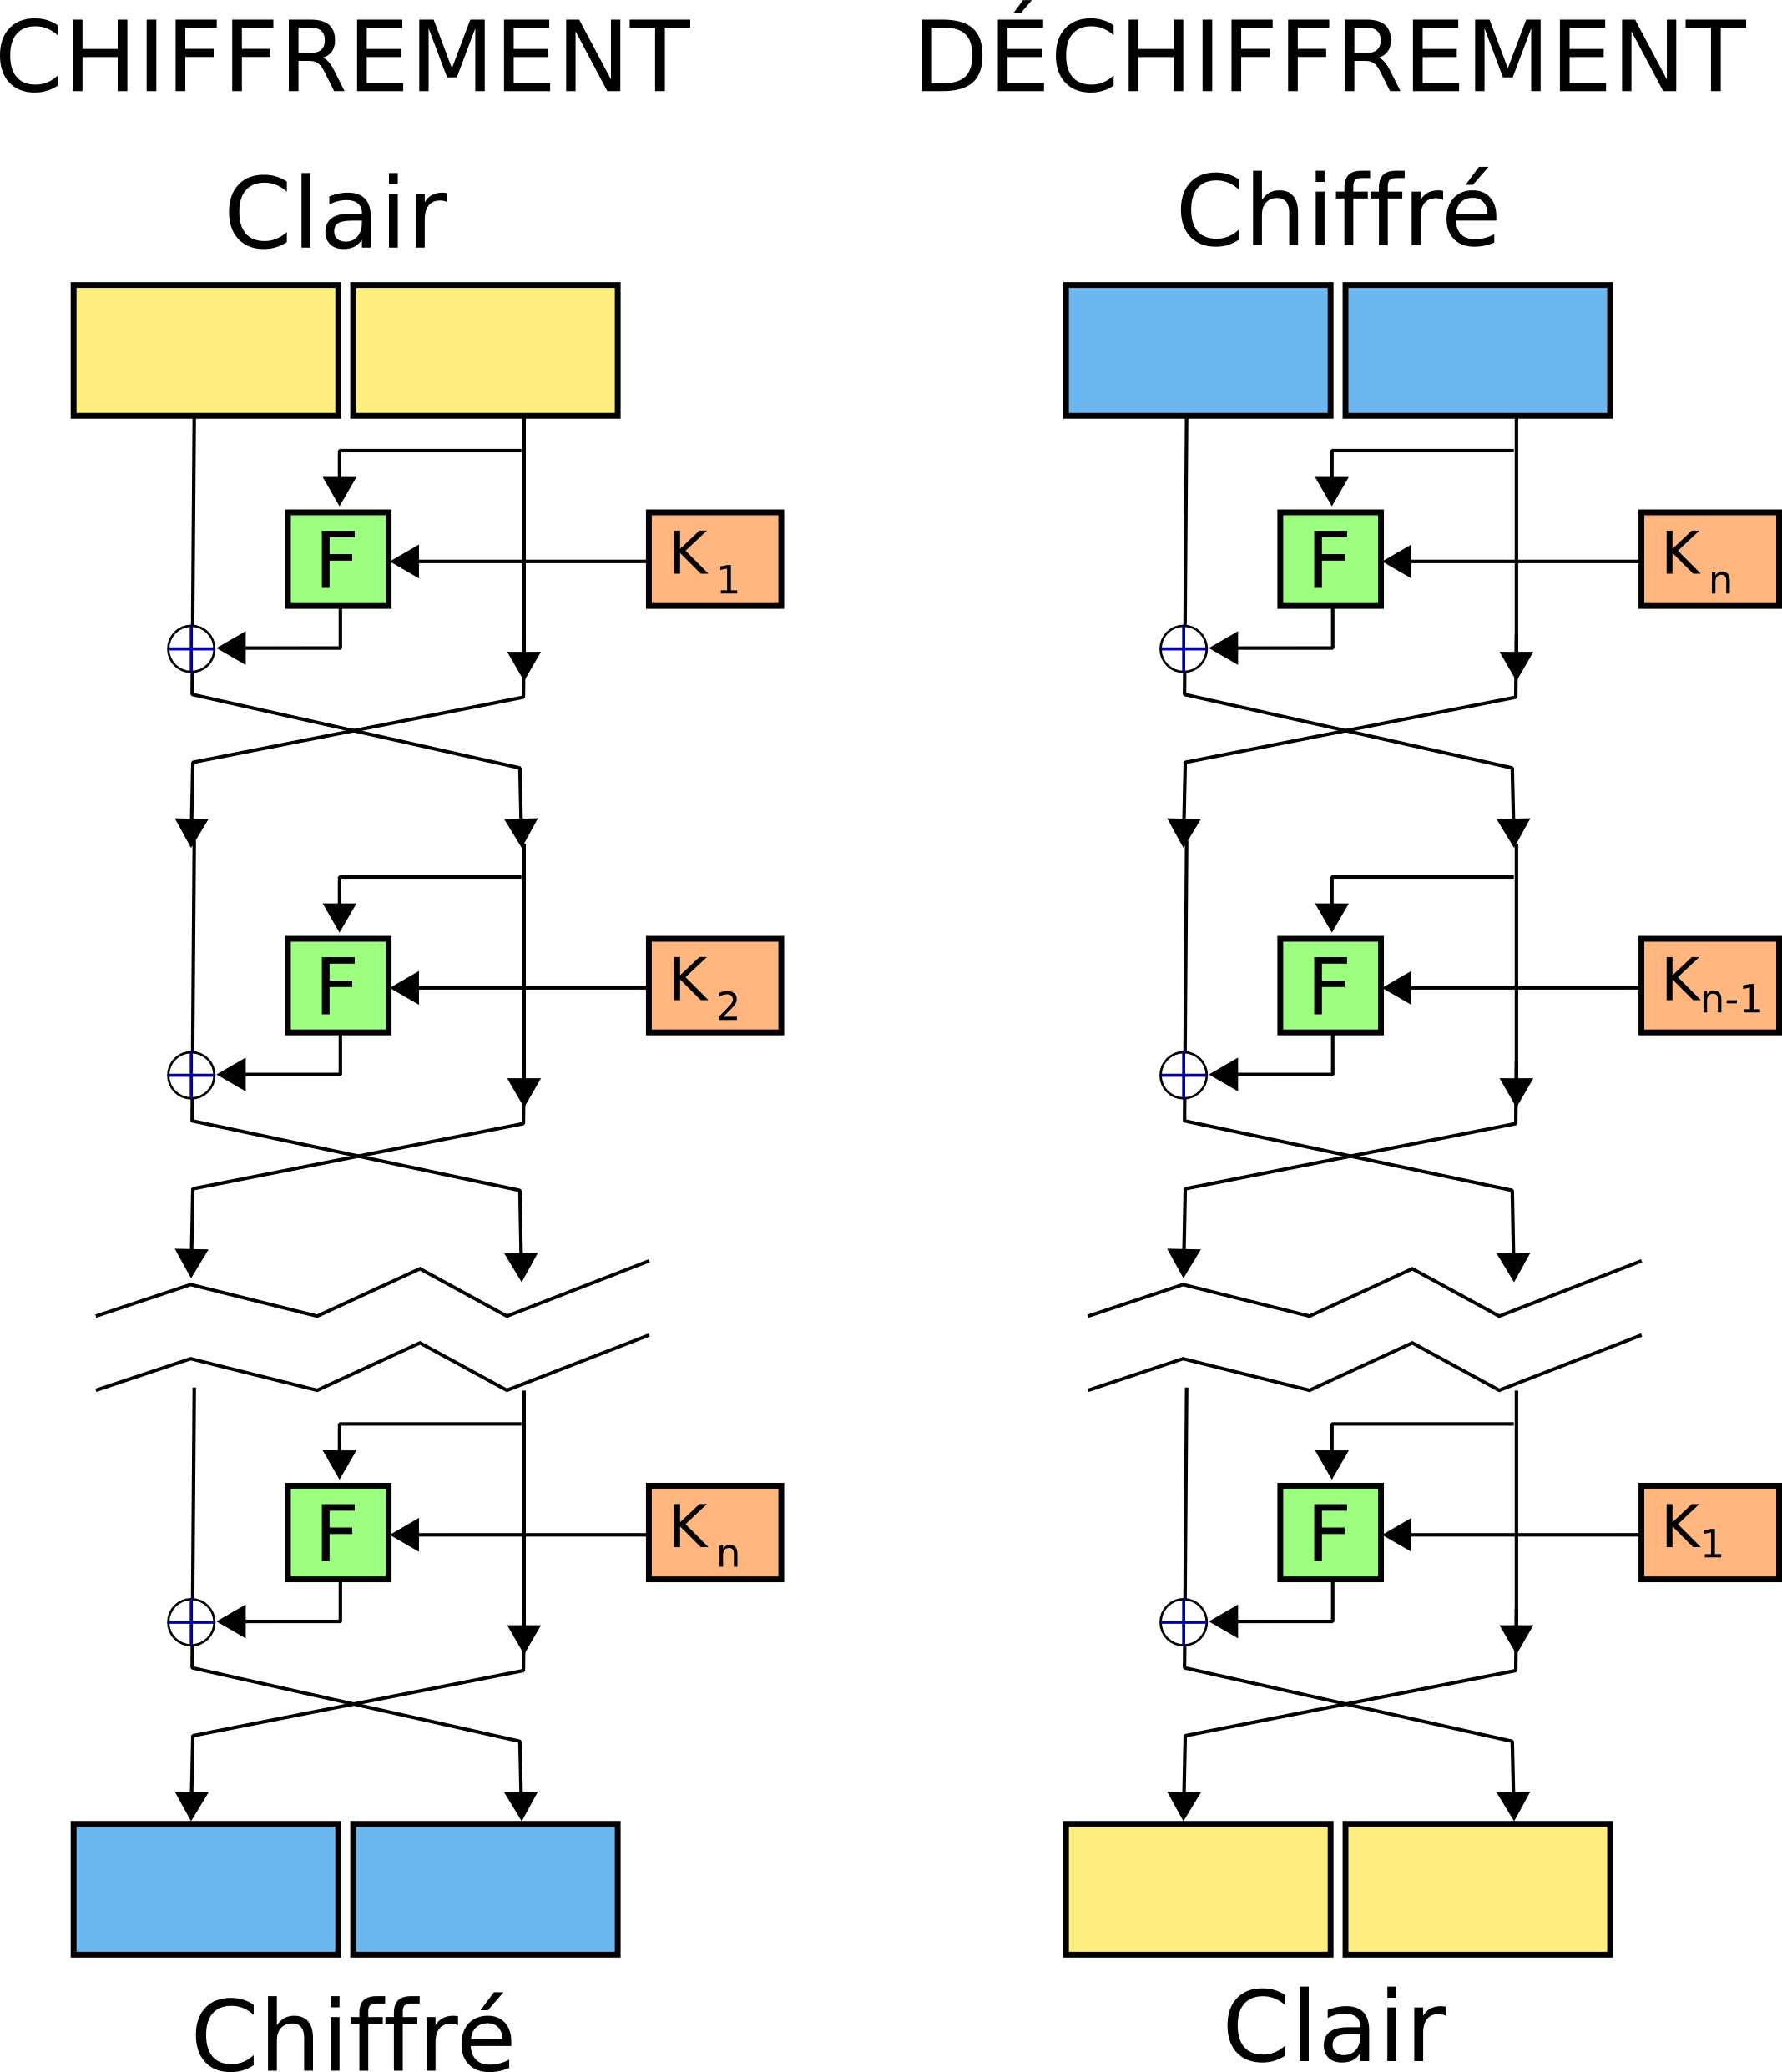
\includegraphics[width=7cm]{images/Reseau_de_feistel.png}
	\caption{Réseau de Feistel}
	\label{Feistel}
\end{figure}

Le chiffrement DES par exemple repose sur ce réseau, et effectue 16 tours.\\
Généralement les deux parties sont équilibrées même si par exemple des algorithme comme MacGuffin de Bruce Schneier utilise un réseau non équilibré.

\subsection{RSA-OAEP}
Dans la PKCS\#1 est décrit le standard de RSA-OAEP. RSAES-OAEP est le terme plus facilement utilisé dans le document : RSA Encryption Scheme OAEP.\\
Il regroupe les primitives RSAEP et RSADP : respectivement RSA Encryption Protocole et RSA Decryption Protocole.

\subsubsection{RSAES-OAEP-ENCRYPT}
Options :
\begin{description}
	\item [Hash :] fonction de hachage (\texttt{hLen} contient la longueur en octets de la sortie de fonction de hachages);
	\item [MGF :] fonction de génération de masque.\\
\end{description} 
Entrée :
\begin{description}
	\item [(n, e) : ] destinataire de la clef publique RSA (\texttt{k} contient la longueur en octets du modulo RSA \texttt{n});
	\item [M : ] message à chiffrer, un chaîne d'octets de longueur \texttt{mLen}, quand \texttt{mLen <= k - 2hLen - 2};
	\item [L : ] champ optionnel à associer au message, la valeur par défaut pour \texttt{L}, si \texttt{L} n'a aucune condition, est la chaîne vide.\\
\end{description}
Sortie :
\begin{description}
	\item [C : ] texte chiffré, une chaîne d'octets de longueur \texttt{k}.\\
\end{description}
Erreurs :  
\begin{itemize}
	\item "\textit{message too long}"; 
	\item "\textit{label too long}".\\
\end{itemize}
Précondition : 
\begin{itemize}
	\item la clef publique RSA \texttt{(n, e)} est valide.\\
\end{itemize}
Étapes:
\begin{enumerate}
	\item vérifier de la longueur:
	\begin{enumerate}
		\item si la longueur de \texttt{L} est plus grande que la longueur limite en entrée de la fonction de hachage ($2^{61} - 1$ octets pour SHA-1), renvoyer "\textit{label too long}" et arrêter;      
		\item si \texttt{mLen > k - 2hLen - 2}, le message "\textit{message too long}" est renvoyé et la fonction est stoppée.\\
	\end{enumerate}
	\item coder EME-OAEP (voir Figure 1 ci-dessous):
	\begin{enumerate}
		\item si l'étiquette \texttt{L} n'est pas spécifiée, laisser \texttt{L} à une chaîne vide. Laisser \texttt{lHash = Hash(L)}, une chaîne d'octets de taille \texttt{hLen} (voir note plus bas);
		\item générer une chaîne d'octets PS consistant en \texttt{k - mLen - 2hLen - 2} d'octets zéro. La taille de \texttt{PS} peut être zéro;
		\item concaténer \texttt{lHash}, \texttt{PS}, un unique octet avec la valeur hexadécimale \textit{0x01}, et le message \texttt{M} pour former un bloc de données DB de longueur \texttt{k - hLen - 1} octets, tel que : \texttt{DB} = \texttt{lHash} \textbar\textbar \texttt{PS} \textbar\textbar \textit{0x01} \textbar\textbar \texttt{M};
		\item générer un une chaîne d'octets aléatoires de longueur \texttt{hLen};
		\item laisser \texttt{dbMask = MGF(seed, k - hLen - 1)};
		\item laisser \texttt{maskedDB = DB xor dbMask};
		\item laisser \texttt{seedMask = MGF(maskedDB, hLen)};
		\item laisser \texttt{maskedSeed = seed xor seedMask};
		\item concaténer un unique octet avec la valeur hexadécimale \textit{0x00}, \texttt{maskedSeed}, et \texttt{maskedDB} pour former un message chiffré \texttt{EM} de longueur \texttt{k} octets tel que \texttt{EM = 0x00} \textbar\textbar \texttt{maskedSeed} \textbar\textbar \texttt{maskedDB}.\\
	\end{enumerate}
	\item chiffrement RSA :
	\begin{enumerate}
		\item convertir le message codé \texttt{EM} en un entier représentatif du message \texttt{m} (voir section 4.2) : \texttt{m = OS2IP (EM)};
		\item appliquer la primitive de chiffrement \texttt{RSAEP}(Section 5.1.1) avec la clef RSA publique (n, e) pour produire un entier c représentatif du message chiffré : \texttt{c = RSAEP ((n, e), m)};
		\item convertir le texte chiffré représentatif \texttt{c} en un texte chiffré \texttt{C} de taille \texttt{k} octets (voir Section 4.1) : \texttt{C = I2OSP (c, k)}.\\
	\end{enumerate}
	\item envoyer en sortie le texte chiffré \texttt{C}.\\
\end{enumerate}
\paragraph{Note}  Si \texttt{L} est une chaîne vide, la valeur du hash correspondante \texttt{lHash} a la représentation hexadécimale suivante pour différents choix de hash :


\begin{table}[H]
\centering
\begin{tabularx}{17cm}{Xllllll}
SHA-1: &  (0x)da39a3ee & 5e6b4b0d & 3255bfef & 95601890 & afd80709 & \\
SHA-256: 	& (0x)e3b0c442 	& 98fc1c14 	& 9afbf4c8 	& 996fb924 	& 27ae41e4 	& 649b934c\\
			& a495991b 		& 7852b855 	& 			& 			& 			&\\
SHA-384: 	& (0x)38b060a7 	& 51ac9638  	& 4cd9327e 	& b1b1e36a 	& 21fdb711 	& 14be0743\\
			& 4c0cc7bf 		& 63f6e1da 	& 274edebf 	& e76f65fb 	& d51ad2f1 	& 4898b95b\\
SHA-512: 	& (0x)cf83e135 	& 7eefb8bd 	& f1542850 	& d66d8007 	& d620e405 	& 0b5715dc\\
			& 83f4a921 		& d36ce9ce 	& 47d0d13c 	& 5d85f2b0 	& ff8318d2 	& 877eec2f\\
			& 63b931bd 		& 47417a81 	& a538327a 	& f927da3e	&			&\\
\end{tabularx}
\caption{représentations hexadécimales}
\label{repres_hexa}
\end{table}

\begin{description}
   	\item SHA-1:   (0x)da39a3ee 5e6b4b0d 3255bfef 95601890 afd80709;
   	\item SHA-256: (0x)e3b0c442 98fc1c14 9afbf4c8 996fb924 27ae41e4 649b934c\\
                a495991b 7852b855;
   	SHA-384: (0x)38b060a7 51ac9638 4cd9327e b1b1e36a 21fdb711 14be0743\\
                4c0cc7bf 63f6e1da 274edebf e76f65fb d51ad2f1 4898b95b;
   	SHA-512: (0x)cf83e135 7eefb8bd f1542850 d66d8007 d620e405 0b5715dc\\
                83f4a921 d36ce9ce 47d0d13c 5d85f2b0 ff8318d2 877eec2f\\
                63b931bd 47417a81 a538327a f927da3e.\\
\end{description}

\begin{figure}[H]
	\centering
	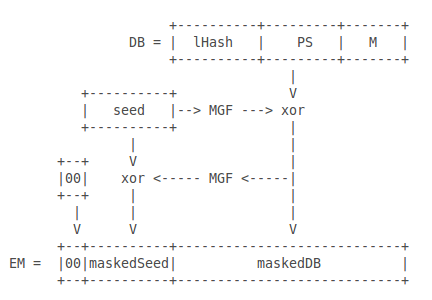
\includegraphics[width=10cm]{images/schema.png}
	\caption{opération de chiffrement EME-OAEP}
	\label{fig21}
\end{figure}

\texttt{lHash} est le hash de l'étiquette optionnelle \texttt{L}. L'opération de déchiffrement suivant inverse les étapes pour retrouver \texttt{M} et vérifier \texttt{lHash} et \texttt{PS}.


\subsubsection{RSAES-OAEP-DECRYPT (K, C, L)}

Options :
\begin{description}
	\item [Hash :] fonction de hachage (\texttt{hLen} contient la longueur en octets de la sortie de la fonction de hachage);
   	\item [MGF :] fonction de génération du masque.\\
\end{description}
Entrée :
\begin{description}
   	\item [K :] destinataire de la clef privée RSA (\texttt{k} contient la longueur en octets du modulo RSA \texttt{n});
   	\item [C :] texte chiffré à déchiffrer, une chaîne de caractères de taille \texttt{k}, où \texttt{k = 2hLen + 2};
   	\item [L :] champ optionnel dont l'association avec le message doit être garantie; la valeur par défaut pour \texttt{L} est, si pas de spécification, une chaîne vide.\\
\end{description}
Sortie :
\begin{description}
    \item [M :] message, une chaîne d'octets de longueur \texttt{mLen}, où \texttt{mLen <= k - 2hLen - 2}.\\
\end{description}
Erreur : 
\begin{itemize}
	\item "decryption error";
\end{itemize}
Étapes :
\begin{enumerate}
	\item Vérification des longueurs :
	\begin{enumerate}
     	\item Si la longueur de \texttt{L} est supérieur à la taille limite en entrée de la fonction de hachage (\texttt{$2^{61 - 1}$} octets pour SHA-1), renvoie "decryption error" et s'arrête;
		\item Si la longueur du texte chiffré \texttt{C} n'est pas de \texttt{k} octets, renvoie "decryption error" et s'arrête;
     \item Si \texttt{k < 2hLen + 2}, renvoie "decryption error" et s'arrête.\\
	\end{enumerate}
	\item déchiffrement RSA :
	\begin{enumerate}
     	\item Convertir le texte chiffré \texttt{C} en un entier \texttt{c} représentatif du message chiffré (voir Section 4.2) : \texttt{c = OS2IP (C)};
     	\item Appliquer la primitive de déchiffrement \texttt{RSADP} à la clef privée RSA \texttt{K} et au message chiffré représentatif \texttt{c} pour produire un entier \texttt{m} représentatif du message clair : \texttt{m = RSADP (K, c)};\\
      	si RSADP renvoie "ciphertext representative out of range" (signifie que \texttt{c >= n}), renvoie "decryption error" et s'arrête;
      	\item convertir le message représentatif \texttt{m} en un un message déchiffré \texttt{EM} de longueur \texttt{k} octets (voir Section 4.1) : \texttt{EM = I2OSP (m, k)}.\\
	\end{enumerate}
	\item déchiffrement EME-OAEP :
	\begin{enumerate}
     	\item si l'étiquette \texttt{L} n'est pas spécifiée, laisser \texttt{L} à une chaîne vide, laisser \texttt{lHash = Hash(L)}, une chaîne d'octets de longueur \texttt{hLen} 
      	\item séparer le message encodé \texttt{EM} dans un seul octet \texttt{Y}, une chaîne d'octets \texttt{maskedSeed} de longueur \texttt{hLen}, et une chaîne d'octets \texttt{maskedDB} de longueur \texttt{k - hLen - 1} telle que \texttt{EM = Y \textbar\textbar maskedSeed \textbar\textbar maskedDB};
      	\item laisser \texttt{seedMask = MGF(maskedDB, hLen)};
      	\item laisser \texttt{seed = maskedSeed xor seedMask};
      	\item laisser \texttt{dbMask = MGF(seed, k - hLen - 1)};
      	\item laisser \texttt{DB = maskedDB xor dbMask};
      	\item séparer \texttt{DB} en une chaîne d'octet \texttt{lHash} de longueur \texttt{hLen}, une chaîne de padding (possiblement vide) \texttt{PS} consistant en des octets hexadécimaux de valeur \textit{0x00}, et un message \texttt{M} tel que \texttt{DB = lHash \textbar\textbar PS \textbar\textbar 0x01 \textbar\textbar M};
		 \\ s'il n'y a pas d'octet avec la valeur hexadécimale \textit{0x01} pour séparer \texttt{PS} de \texttt{M}, si \texttt{lHash} n'est pas égal à \texttt{lHash}, ou si \texttt{Y} n'est pas une sortie non nulle, renvoyer "decryption error" et s'arrêter.\\
	\end{enumerate}
	\item Renvoyer le message M.\\
\end{enumerate}
\paragraph{Note}  Il faut faire attention qu'un adversaire ne puisse distinguer les différentes erreurs dans les conditions de l'étape 3, que ce soit par un message d'erreur, ou un temps de réponse différent, ou, plus généralement, apprendre une information partielle à propos du message en clair \texttt{EM}. Sinon un adversaire peut être en mesure d'obtenir des informations utiles sur le déchiffrement du texte chiffré \texttt{C}, conduisant à une attaque à chiffré choisi telle que celle observée par Manger.
   
\subsubsection{RSAES-PKCS1-v1\_ 5}

   RSAES-PKCS1-v1\_5 combine les primitives RSAEP et RSADP avec la méthode de codage EME-PKCS1-v1\_ 5. Il est mathématiquement équivalent au schéma de chiffrement dans la PKCS \# 1 v1.5. RSAES-PKCS1-v1\_ 5 peut fonctionner sur des messages de longueur supérieure à \texttt{k - 11} octets (\texttt{k} est la longueur en octets du modulo RSA), bien qu'il faille faire attention aux attaques portant sur les faibles exposants RSA menée par Coppersmith, Franklin, Patarin, and Reiter quand les longs messages sont chiffrés (voir le troisième point dans les notes ci-dessous).\\
En règle générale, l'utilisation de ce schéma pour chiffrer un message arbitraire, en opposition à une clef générée aléatoirement, n'est pas recommandé.\\   
Il est possible de générer des textes chiffrés RSAES-PKCS1-v1\_5 valides sans connaître les messages clairs correspondants, avec une probabilité raisonnable de réussite.\\
Cette possibilité peut être exploitée dans une attaque à chiffré choisi, comme montré en [6]. Par conséquent, si RSAES-PKCS1-v1\_5 doit être utilisé, certaines contre mesures faciles à implémenter devraient être mises en place afin de contrecarrer l'attaque trouvée en [6].\\
Des exemples typiques comprennent l'ajout de la structure des données à encoder, le contrôle rigoureux de la conformité des PKCS\# 1v1.5 (et d'autres redondance) dans les messages déchiffrés, et la consolidation des messages d'erreur dans un protocole client-serveur basée sur PKCS \# 1 v1.5. Ils peuvent tous être des contre-mesures efficaces et n'entraînent pas de changement à un protocole n\degres 1 sur la base de v1.5-PKCS. Il a été récemment montré que la sécurité du protocole SSL / TLS handshake, qui utilise RSAES-PKCS1-v1\_5 et certaines contre-mesures, peut être liée à une variante du problème RSA.\\
  
\paragraph{Note}  Les passages suivants décrivent des recommandations concernant l'utilisation de RSAES-PKCS1-v1\_5. Les recommandations de la version 1.5 de ce document sont inclues ainsi que de nouvelles recommandations motivées par les avancées de cryptanalyse durant les années suivantes.
\begin{itemize}
	\item il est recommandé que les octets pseudo aléatoires soient générés indépendamment pour chaque processus de chiffrement, en particulier si la même donnée est en entrée pour plus d'un processus de chiffrement. Les résultats de Haastad sont une des motivations pour cette recommandation;
	\item La chaîne de padding \texttt{PS} est d'une longueur d'au moins 8 octets, ce qui est une condition de sécurité pour les opérations sur les clefs publiques, et qui rend difficile pour les attaquants de récupérer les données en essayant tous les blocs chiffrés possibles.
	\item les octets pseudo aléatoires peuvent aussi aider à contrecarrer une attaque grâce à Coppersmith et al. quand la taille du message à chiffrer est gardé petit. L'attaque marche sur les petits exposants RSA quand des messages similaires sont chiffrés avec la même clef publique. Plus spécifiquement, une façon peut être, quand deux entrées RSAEP correspondent sur une large portion de bits (8/9) et qu'un petit exposant RSA est utilisé (e = 3) pour chiffrer les deux, il peut être possible de retrouver les entrées avec l'attaque. Une autre façon d'attaquer est couronnée de succès pour déchiffrer un seul texte chiffré, quand une large proportion (2/3) des entrées de RSAEP est déjà connue. Pour des applications typiques, le message à chiffrer est court (par exemple une clef symétrique de 128 bits) donc peu d'informations seront connues ou en commun entre deux messages pour permettre l'attaque. Cependant, si un long message est chiffré, ou si une partie du message est connu, alors l'attaque peut fonctionner. Dans tous les cas, le schéma  RSAES-OAEP surmonte l'attaque.\\
\end{itemize}

\subsection{CBC : \textit{Cipher Block Chaining}}
C'est un mode de chiffrement qui a été très utilisé : enchaînement des blocs.\\
Sur chaque bloc, un OU exclusif avec le chiffrement du bloc précédent est appliqué. Un vecteur d'initialisation est lui aussi utilisé. Contrairement au mode ECB, les blocs identiques ne seront pas chiffrés de la même façon. On ne pourra donc pas repérer de chaîne de caractères récurrentes aussi facilement. Ce mode de chiffrement possède plusieurs inconvénients : 
\begin{itemize}
	\item un chiffrement de plusieurs blocs en parallèles est impossible (puisque chaque bloc dépend du chiffrement du précedent). Déchiffrer avec un IV incorrect entraînera une corruption dans le premier bloc en clair, mais les blocks suivants seront corects. C'est parce qu'un texte claire peut être récupéré grâce à deux blocs adjacents du texte chiffré. Le déchiffrement, contrairement au chiffrement, peut donc être parallélisé. À noter que si un seul bit change dans le texte chiffré, le bloc clair correspondant est complètement corrompu.
	\item Si une erreur se produit sur un bloc, elle sera répercutée sur tous les suivants. La propagation d'erreur n'est pas limitée.
\end{itemize} 
\begin{figure}[H]
	\centering
	
\includegraphics[width=13cm]{images/CBC_chiff.png}
	\caption{Chiffrement CBC}
	\label{CBC_chiff}
\end{figure}

\begin{figure}[H]
	\centering
	
\includegraphics[width=13cm]{images/CBC_dechiff.png}
	\caption{Déchiffrement CBC}
	\label{CBC_dechiff}
\end{figure}

Il a d'abord été défini par le NIST dans le FIPS 81 (\url{http://www.itl.nist.gov/fipspubs/fip81.htm}). Le standard a été publié en 1981.


\section{Audits}
	\subsection{Audit 3.1 : Les "Manger's attack" sur RSA-OAEP}
		\subsubsection{Normes visées}

		A remplir.
	
		\subsubsection{Faille}
		
			RSA-OAEP peut être soumis à une attaque nommée "Mangers Attack" selon son implantation \cite{mangers2010falko}. OpenSSL semble être vulnérable à une attaque de ce type, à base de "prédictions" par injections de fautes. La vulnérabilité semble être très récente puisqu'elle fonctionne sous OpenSSL 1.0.0.\\

			
			Le padding OAEP devait pallier le problème d'insécurité que causait le padding PKCS\#1 v1.5 (attaque à chiffré choisi) \cite{bleichenbacherPCKS}. OpenSSL a tout de même pris en compte cette vulnérabilité et a placé des contres-mesures efficaces.	La Technische Universität Darmstadt (Allemagne) explique en détail comment sont implémentées ces contres-mesures et montre que dans certains cas l'attaque reste possible. Enfin, elle apporte ses propres contre-mesures.\\
			
			On peut noter que plusieurs librairies sont vulnérables à une attaque de Manger qui consiste à contrôler la taille des paramètres à haché, mais que l'implantation de RSA-OAEP d'OpenSSL ne le permet pas.La raison est que le décodage OAEP est linéaire quelque soit la taille des paramètres et les erreurs survenues. 	Il semble également y avoir un problème avec l'OAEP\_padding sur le chiffrement RSA. Bill Nickless recommande l'utilisation de PKCS\_padding. \cite{sourceforgeRSAbroken}	\\
		
		
		\subsubsection{Implémentation}
			
			\paragraph{Configuration visée.\\}
			
			L'étude a été réalisée sur la librairie OpenSSL-1.0.0.
			
			\paragraph{Fonction.\\}
			
			La fonction auditée se nomme RSA\_padding\_check\_PKCS1\_OAEP() (cf. \textit{Listing} \ref{rsaoaep}) et est accessible à partir du chemin \texttt{openssl/crypto/rsa/rsa\_oaep.c}.
		
		
			\begin{lstlisting}[style=customc,caption=rsa\_oaep.c,
			label=rsaoaep]
				lzero = num - flen;
				if (lzero < 0)
				{
					/* signalling this error immediately after detection might allow
					* for side-channel attacks (e.g. timing if 'plen' is huge
					* -- cf. James H. Manger, "A Chosen Ciphertext Attack on RSA
	Optimal
					* Asymmetric Encryption Padding (OAEP) [...]", CRYPTO 2001),
					* so we use a 'bad' flag */
					bad = 1;
					lzero = 0;
					flen = num; /* don't overflow the memcpy to padded_from */
				}
			\end{lstlisting}
		
			Le développeur n'a pas considéré qu'il y avait un grand danger dans le code de contre-mesures.\\
			Pourtant l'étude confirme qu'il y a un décalage de temps possible, certes léger mais qui peut entraîner une attaque en "branch prediction" (qui peut se traduire en prédiction par dérivation).\\
			
		\subsubsection{Conclusion}
		
			Il n'y a pas vraiment de quoi s'alarmer, cette attaque est en pratique infaisable sur un serveur car il y a suffisamment de variations de délais (différences de CPU, opérations multi-tâches, connexions réseaux, etc...) pour éviter une attaque par timing. Cependant, sur des systèmes embarqués l'attaque peut être réalisable, et il serait plus prudent de pallier ce problème.
			
	\subsection{Audit 3.2 : Chiffrement SSLv3 ou TLS 1.0 en mode CBC}
		\subsubsection{Normes visées}
	
			A remplir.	
	
		\subsubsection{Description de la faille}
			
			En Septembre 2011, une attaque en man in the middle très efficace a vu le jour contre les protocoles SSLv3 et TLS 1.0. \cite{ekr2011beast} \cite{imperial2011beast} \cite{goodin2011beast} \cite{gallagher2011beast}. L'attaque est à clair choisi. Le but étant d'insérer des morceaux de texte clair grâce au navigateur dans la requête chiffrée avec ces protocoles, ceci afin de récupérer les cookies de session.\\
			
			La technique est basique, un individu enregistre plusieurs cookies de session auprès de divers sites officiels (banques, messageries, etc...). Puis, il clique malencontreusement sur du code Java malveillant (publicité, image, etc...). et l'attaque se déroule automatiquement. L'ensemble des cookies est envoyé au serveur malveillant qui n'a plus qu'à déchiffrer les clés de session.\\
			
			La cause viendrait du mode de chiffrement choisi : CBC. SSL/TLS est un protocole qui chiffre un canal de communication.	De ce fait il ne chiffre pas un fichier unique, mais une série d'enregistrements. Il y a deux façons d'utiliser le mode CBC dans ce cas précis :
			\begin{itemize}
			\item Prendre chacun de ces enregistrements indépendamment des autres. Générer un nouveau vecteur d'initialisation à chaque fois.
			\item Traiter ces enregistrements comme un seul objet en les concaténant. Le vecteur d'initialisation est donc choisi aléatoirement pour le premier enregistrement et pour les autres, il aura pour valeur le dernier bloc de l'enregistrement précédent.\\
			
			\end{itemize}
			
			SSLv3 et TLS 1.0 utilisent ce deuxième choix, cela soulève un lourd problème de sécurité.	En 2004, Moeller \cite{moeller2004cbc} trouve une méthode pour exploiter ce mauvais choix afin de récupérer des morceaux de textes clairs. Il y a certes une faille immense, mais peu exploitable. Les grandes entreprises savent (normalement) qu'il ne faut pas utiliser le mode CBC pour du chiffrement SSL/TLS. Et, dans tout les cas, plusieurs navigateurs ne permettent pas ce type d'attaque (c'est le cas de Chrome par exemple).
			
		\subsubsection{Tests}
			
			Nous n'avons pas repris les tests du logiciel BEAST qui s'avère être introuvable sur le Web (celui-ci étant un projet universitaire, développé par un étudiant de l'Université de Versailles). Mais une vidéo de l'exploit est accessible sur YouTube au lien ci-dessous : \\
			
			\textbf{Lien YouTube : } \href{http://www.youtube.com/watch?v=ujz4SXzWK9o} {http://www.youtube.com/watch?v=ujz4SXzWK9o}
		
		\subsubsection{Recommandations}

			La faille existe tant que l'association de ces protocoles avec le mode de chiffrement CBC existe. Même si l'attaque est infaisable sur les navigateurs les plus répandus (Chrome, Firefox, IE, Safari, ...), OpenSSL devrait pouvoir interdire cette association, et ne pas laisser le travail aux navigateurs. 	Mais rien n'empêche l'utilisation de ce chiffrement par un navigateur plus léger, nous pourrons tester cette vulnérabilité lors de notre partie 3 si nous trouvons un navigateur acceptant ce type de chiffrement.				
			
	\subsection{Audit 3.3 : Non-validation des certificats SSL}
		\subsubsection{Normes visées}
	
			A remplir.

		\subsubsection{Description de la faille}
		
			Six chercheurs des universités de Stanford et d'Austin au Texas, analyse une attaque en Man in the Middle autour des certificats SSL sans utilisation d'un navigateur. Le titre est sans appel "Le code le plus dangereux du monde" \cite{validate2012martin}.\\
			
			
			SSL doit permettre d'être sécurisé en toutes circonstances, que le cache DNS soit empoisonné, que les attaquants contrôlent les points d'accès et les routeurs, etc. . Il assure théoriquement trois grands principes de la cryptologie : la confidentialité, l'intégrité et l'authentification. Nous connaissons certaines failles au niveau du navigateur et de l'implantation SSL (voir ci-dessus). Mais il existe également d'autres cas d'utilisation du protocole SSL. Par exemple:
			\begin{itemize}
			\item Administration à distance basé sur le cloud, stockage sécurisé sur le cloud en local.
			\item Transmissions de données sensibles (ex: e-commerce)
			\item Services en ligne comme les messageries électroniques
			\item Authentification via applications mobiles comme Android et iOS\\
			\end{itemize}
			
			L'étude montre que la validation des certificats SSL est casée sur plusieurs applications et librairies dont :
			\begin{itemize}
			\item OpenSSL
			\item JSSE
			\item CryptoAPI
			\item NSS
			\item GnuTLS
			\item etc...\\
			\end{itemize} 
			
			En fait, un attaquant en Man In The Middle peut intercepter le secret entre un client et un serveur utilisant une connexion SSL. Il peut ainsi  récupérer des numéros de carte bancaire, avoir accès à une messagerie, récupérer des mots de passes, etc... La cause principale vient du fait que les développeurs retouchent les librairies cryptographiques à leur façon. En voulant réparer un bug ou en souhaitant rendre SSL compatible avec leurs API, ils injectent de nouvelles vulnérabilités. 	De plus, l'application est souvent propriétaire et payante ce qui rend le déboggage difficile.\\
			
			
			Que ce soit accidentel ou intentionnel, l'une des conséquences les plus graves est la non-validation de certificat sur des contexte où la sécurité est primordiale (e.g. payement en ligne). La faute ne revient pas directement au code d'OpenSSL, mais à une mauvaise utilisation des différentes fonctions et options.\\
			
			
			Voici quelques exemples concrets concernant différentes API : 
			\begin{itemize}
			\item Les services comme Amazon's Flexible Payments Service PHP et PayPal Payments Standard PHP passent le paramètre \texttt{CURLOPT\_SSL\_VERIFYHOST} à true alors que la valeur doit être passée à 2. La conséquence est la désactivation de la validation du certificat
			\item Lynx, un navigateur textuel très connu et souvent utilisé dans le développement d'applications, vérifie les certificats auto-signés seulement si la fonction de validation de certificat GnuTLS retourne une valeur négative. Malheureusement, dans certains cas la fonction peut retourner 0 pour certaines erreurs (dont les certificats signés par une autorité sans confiance).
			\item La librairie SSLSocketFactory de JSSE, très réputée, ne fait pas de vérification si la cypher suite du client vaut NULL ou est une chaîne vide.
			\item Vulnérabilités sur Apache HttpClient, WebSockets, Android, ...
			\item Autres causes célèbres : non reconnaissance des expressions régulières, non vérification du résultat de la validation, désactivation de l'authentification.\\
			\end{itemize}
			
					
		\subsubsection{Difficultés du code OpenSSL}
			

			OpenSSL ne déroge pas à la règle.\\
			Voici quelques vulnérabilités du code :
			\begin{itemize}
			\item Les contraintes de nom x509 ne sont pas correctement validés.
			\item Les applications DOIVENT fournir elles même leur code de vérification de nom d'hôte. Or, des protocoles comme HTTPS, LDAP ont chacun leurs propres notions de validations. Ainsi, Apache Libcloud utilise les librairie Python eux-même utilisant des commandes OpenSSL. Et sa méthode de vérification du nom d'hôte comporte des vulnérabilités pouvant causer des attaques en man in the middle (e.g "google.com" et "oogle.com" vérifie la même expression régulière)
			\item Un programme utilisant OpenSSL peut exécuter la fonction \texttt{SSL\_connect} pour le handshake SSL. Bien que certaines erreurs de validation soient signalées par \texttt{SSL\_connect}, d'autres ne peuvent être vérifier qu'en appelant la fonction \texttt{SSL\_get\_verify\_result}, alors que \texttt{SSL\_connect} se contente de retourner "OK".
			\end{itemize}

		\subsubsection{Exemple : Trillian}

			Trillian est une messagerie cliente instantanée	reliée à OpenSSL pour la sécurisation de l'établissement de connexion. Par défaut OpenSSL ne soulève pas d'exception en cas de certificat auto-signé ou de non-confiance auprès de la chaîne de vérification. A la place, il envoie un drapeau. De plus, il ne vérifie jamais le nom d'hôte.	Si l'application appelle la fonction \texttt{SSL\_CTX\_set} pour initialiser le drapeau \texttt{SSL\_VERIFY\_PEER}, alors \texttt{SSL\_connect} se ferme et affiche un message d'erreur lorsque le certificat n'est pas valide.	Mais Trillian n'initialise jamais ce drapeau.	Par conséquent, \texttt{SSL\_connect} va retourner 1 et le statut de la validation du certificat peut être connu en appelant la fonction \texttt{SSL\_get\_verify\_result}.	Encore une fois, Trillian n'appelle pas cette fonction.	Les conséquences sont très lourdes : vols de mots de passes, compromissions de services, révélations des paramètres de sécurité, etc...\\
			

			L'étude montre que l'attaque est possible sur la version 5.1.0.19 et antérieure de Trillian.

		\subsubsection{Conclusion}

			Les chercheurs nous donnent alors plusieurs leçons à retenir, dont voici quelques points :
			\begin{itemize}
			\item Premièrement, les vulnérabilités doivent être trouvées et réparées lors des phases de tests. Certaines se trouvent très facilement si les procédures de tests sont bien réalisées. 
			\item Deuxièmement, la plupart des librairies SSL ne sont pas \textbf{sûres par défaut}, laissant le choix de la sécurité aux applications de plus haut niveau avec choix des options, choix de la vérification de l'hôte, choix d'interprétation des résultats.
			\item Troisièmement, même les librairies SSL sûrs par défaut peuvent être mal utilisées par des développeurs changeant les paramètres par défaut par des paramètres non sécurisés. La cause peut venir d'une \textbf{mauvaise documentation} ou d'une mauvaise formalisation de la part de l'API. Les API devraient entre autre proposer des abstractions de haut niveau pour les développeurs comme des tunnels d'authentification, plutôt que de les laisser traiter des détails de bas niveau comme la vérification du nom d'hôte.\\
			\end{itemize}

			Nous conseillons surtout une meilleure documentation d'OpenSSL, et des rapports d'erreurs d'interfaces plus simples et plus consistants afin d'éviter les erreurs d'interprétation. L'idée des chercheurs de proposer des abstractions de haut niveau pour les applications semblent être une très bonne idée.
		

\section{Recommandations générales}
\chapter{Signature et authentification}
\section{Définitions et contexte}

Une signature digital utilise le concept du traditionnel signature sur papier et le tourne en une empreinte électronique. Cette empreinte est un message encodé et est unique pour chaque document et le signataire. La signature permet alors de garantir l'authenticité du signataire pour son document. Toute modification dans le document après l'avoir signé rend la signature invalide, ce qui protège alors contre les fausses informations et la contrefaçon des signatures.\\

De ce fait, il est important de faire attention à toute les formes de vulnérabilités des signatures afin de comprendre les attaques possible sur la contrefaçon des signatures. Dans cette partie est consacré à la bonne compréhension et implémentation qui sont définie dans la RFC, afin de se prémunir des différentes attaques possible. On verra, cependant, qu'il existe quand même des failles au niveaux des injections, surtout lorsque la librairie dépend trop du matérielle. 


\section{Audits}
	\subsection{Audit 1 : Attaque par injection de fautes sur les certificats RSA}
		\subsubsection{Normes visées}
Dans la RFC 3447 \cite{rfc3447}, la signature est décrite telle une primitive de signature qui produit la représentation de la signature depuis un message sous le contrôle d'une clef privée. La vérification se fait alors en récupérant la représentation du message depuis la représentation de la signature sous le contrôle de la clef publique correspondante.\\

La signature se déroule en  deux opérations qui sont la génération et la vérification. L'opération de génération consiste donc à générer une signature depuis un message avec la clef privée de l'utilisateur (signataire) et l'opération de vérification consiste à vérifier la signature en se basant sur le message en utilisant la clef publique du signataire. 
Ce schéma peut être utilisé dans de multiples applications telles que les certificats X.509.\\


La norme spécifie deux types de schéma de signature qui sont :
\begin{itemize}
\item \texttt{RSASSA-PSS}
\item \texttt{RSASSA-PKCS1-v1\_5} \\
\end{itemize}

Même si aucune attaque n'est connue contre \texttt{RSASSA-PKCS1-v1\_5},  \texttt{RSASSA-PSS} est recommandé dans l'intérêt d'augmenter la robustesse d'un système. \texttt{RSASSA-PKCS1-v1\_5} est toujours inclue pour des raisons de compatibilités avec les applications existantes et, même si elle est toujours appropriée dans les nouvelles applications, une transition vers \texttt{RSASSA-PSS} est encouragée.\\ 


La norme décrit un modèle général à suivre (qui est également utilisé pour IEEE Std 1363-2000) combinant les primitives de signature et de vérification avec une méthode d'encodage sur les signatures. L'opération de génération de signature applique une opération d'encodage de message à un message pour produire un message encodé, qui est ensuite converti en un entier représentatif du message. Une primitive de signature est alors appliquée sur la représentation du message pour produire la signature.\\ 


Dans le sens inverse, l'opération de vérification de signature applique une primitive de vérification de signature à la signature pour récupérer la représentation du message, qui est alors convertie dans un message de chaîne de caractères encodée. L'opération de vérification est appliquée au message et au message encodé pour déterminer s'ils  consistent bien en  l'un et l'autre.\\ 


\paragraph{RSASSA-PSS : \\}
\texttt{RSASSA-PSS} combine les primitives \texttt{RSASP1} et \texttt{RSAVP1} avec la méthode d'encodage \texttt{EMSA-PSS}. La longueur du message sur laquelle \texttt{RSASSA-PSS} peut travailler est soit illimité, soit contrainte par une très grande valeur, dépendant de la fonction de hachage. Contrairement à \texttt{RSASSA-PKCS1-v1\_5}, un identificateur de fonction de hachage n'est pas inclue dans le message encodé par \texttt{EMSA-PSS}. De ce fait, en théorie, il est possible pour un attaquant de substituer une autre fonction de hachage ( potentiellement plus faible) que celle sélectionnée par le signataire. Il est alors recommandé que la fonction de génération de masquage d'\texttt{EMSA-PSS}  soit basée sur la même fonction de hachage. De cette façon, l'encodage de tout entier sera dépendant de la fonction de hachage et il sera plus difficile pour un adversaire de substituer une autre fonction que ce qui a été sélectionné par le signataire.\\


La comparaison entre fonctions de hachage est seulement utilisée pour empêcher la substitution de fonction de hachage, et n'est pas nécessaire si la fonction de hachage est substituée d'une autre façon (e.g., le vérificateur n'accepte qu'une fonction de hachage désignée).\\ 


Ce qui est différent pour \texttt{RSASSA-PSS} des autres méthodes de signature RSA, c'est qu'il est probabiliste plutôt que déterministe, du fait de  l'incorporation d'un aléa. Cette valeur d'aléa augmente la sécurité de la méthode. Cependant, le fait que la valeur soit aléatoire n'est pas critique pour la sécurité. Dans les situations où l'aléatoire n'est pas possible, une valeur fixe ou une séquence de nombre peut être employée plutôt, et avec une sécurité similaire.

		\subsubsection{Description de la faille}
		
			L'Université du Michigan a réussi l'exploit de récupérer la clé privée d'un certificat RSA en un peu plus de 100h \cite{andrea2010RSA} \cite{opensslvuln2010}. 	L'attaque fonctionne par injection de fautes \cite{fault2008lawson} sur la méthode d'authentification. La technique est donc très poussée, mais le résultat en vaut la chandelle. L'injection de faute doit se faire sur quelques bits pour ne pas faire dysfonctionner le système tout entier. Les signatures erronées produites révéleront de l'information sur la clé privée. Avec le bon matériel et 100h d'attente, la clé peut être reforgé.\\

			La technique consite à renseigner de fausses signatures afin de vérifier les fautes avec la clé publique de la machine. Lorsque la signature est identifié comme fausse, elle est envoyé à un analyseur contenant l'algorithme du \textit{Listing} \ref{windowssearch}

			\begin{lstlisting}[style=customc,caption=window\_search.c, label=windowssearch]
			window\_search (m, s, e, win\_size, win\_idx) {
				found = 0;
				for(d[win\_idx] in [0..2^win\_size-1];
					sqr\_iter in [0..win\_size-1];
					fault in [0..card(bits(d))-1]) {
						found += test\_equation 10(m, s, e,
						win\_idx, d[win\_idx], sqr\_iter, fault loc)
					}
				if (found == 1) 
					return d[win\_idx]
				else 
					return -1
			}
			\end{lstlisting}

			$d$ : fenêtre, $win\_size$ : taille fixé sur la fenêtre, w$in\_idx$ : index de la fenêtre. Et $m$, $s$, $e$ des entiers pour l'opération d'exponentiation modulaire :
			$$ m^e [s]$$

			En contrôlant le voltage, on arrive à savoir qu'un bit en particulier est mauvais. Bit après bit on reconstruit la clé privée, avec une signature erronée pour chacun des exposant de toute les fenêtres. L'étude montre que 650 signatures corrompues suffisent pour retrouver 100\% d'une clé privée RSA de 1024 bits. 

		
		\subsubsection{Implémentation}
			
			\paragraph{Configuration utilisée.\\}
			
			Le logiciel utilisée pour l'étude est OpenSSL 0.9.8i. L'attaque se fait sur la librairie d'authentification OpenSSL sous un système SPARC Linux qui implémente FPGA pour les systèmes cartes à puces.

			\paragraph{Fonction Fixed-window modular exponentiation.\\}

			Cette fonction est accessible dans plusieurs fonctions de chiffrement :
			\begin{itemize}
			\item RSA
			\item ElGamal
			\item DSA
			\item Diffie-Hellman
			\item etc...
			\end{itemize}
		
			Elle garantit des opérations en temps constant afin d'éviter des attaques par timing, et elle reste très performante. Elle s'apparente à la technique square-and-multiply à la seule différence qu'elle utilise des fenêtres de largeur $w$ bits, et partitionne l'exposant dans ces fenêtres au lieu d'examiner l'exposant pour différentes opérations comme square-and-multiply. \\

			C'est le fait que la fenêtre soit fixe qui la rend insensible à une attaque par timing.\\

			L'algorithme FWE est donnée en \textit{Listing} \ref{fwe}
		
			\begin{lstlisting}[style=customc,caption=fwe.c, label=fwe]
				FWE(m, d, n, win_size) {
					num_win = card(bits(d)) / win_size;
					acc = 1;
					for(win_idx in [num_win-1..0])
						for(sqr_iter in [0..win_size-1])
							acc = (acc * acc) mod n;
						d[win_idx] =
							bits(d, win_idx * win_size, win_size);
						acc = (acc * m^d[win_idx]) mod n;
					return acc;
				}
			\end{lstlisting}
		

			L'inconvénient de cet algorithme est qu'il utilise plus de 1000 multiplications. Or, il est connu que pour une attaque par injection de fautes, la multiplication est l'opération la plus sensible en cas de dégradation du microprocesseur. \textit{"The fixed-window exponentiation algorithm in the OpenSSL library does not validate the correctness of the signature produced before sending it to the client, a vulnerability that we exploit in our attack"}\\
			

		\subsubsection{Conclusion}

			Lorsque le système est vulnérable, OpenSSL ne le détecte pas forcément. Le risque est donc très fort, et les contre-mesures sont parfois difficile à trouver dans les phases de tests. Toutefois, cette étude soulève un choix de programmation qui semble à première vue anodin, mais qui peut avoir de lourdes conséquences.\\

			Malheureusement, il faut pouvoir contrôler la machine (en ayant un accès au BIOS par exemple) pour pouvoir exploiter cette faille car il faut pouvoir toucher directement à l'alimentation de la faille.\\

			Cependant, cette erreur n'est pas à prendre à la légère, car une attaque à base de faiseaux lumineux est en cours de développement afin de réaliser cette attaque à distance.
		
\subsection{Audit 2 : Malformation des signatures DSA/ECDSA}
		\subsubsection{Normes visées}

		La RFC R979 \cite{rfc6979} définie l'utilisation de DSA (\textit{Digital Signature Algorithm}) et ECDSA (\textit{Elliptic Curve Digital Signature Algorithm}) de façon déterministe. DSA et ECDSA sont deux standards de signature digital qui offrent l'intégrité et authenticité dans de nombreux protocoles.\\

		Une caractéristique de DSA et ECDSA est qu'ils ont besoin de produire, pour chaque génération de signature, une valeur aléatoire toute fraîche (k). Pour une bonne sécurité, k doit être choisi aléatoirement et uniformément depuis un groupe d'entier modulaire, en utilisant un processus cryptographiquement sûre. Même une petite erreur dans le processus peut devenir une attaque sur la méthode de signature. De ce fait, un système qui génère mal ou pas suffisamment d'entropie lors de la génération d'un nombre aléatoire peut poser de grosse faille dans le déploiement du schéma de signature DSA et ECDSA.\\

		Cette méthode d'utilisation de l'aléatoire avec DSA et ECDSA fait son implémentation plus difficile à tester. Les tests automatiques ne sont pas fiable lorsqu'il s'agit de détecter si implémentation utilise une source aléatoire de grande qualité. De ce fait, le processus d'implémentation est alors plus vulnérable à un échec catastrophique, souvent découvert après le déploiement du système et suite à des attaques réussies.\\

		Il est possible de retourner DSA et ECDSA en une utilisation déterministe en utilisant un processus déterministe de génération d'une valeur "aléatoire", k. Ce processus doit remplir quelques caractéristiques cryptographique afin de maintenir les propriétés de vérifiabilité et d'infalsifiabilité attendues par cette méthode de signature. De ce fait, pour une personne ne connaissent pas la clef privée de la signature, la transformation du message en valeur correspondante, k, doit être calculatoirement indiscernable du retour de la fonction aléatoire et uniforme.
		
		\subsubsection{Description de la faille}
			
		En 2008, une vulnérabilité sur la malformation des signatures survient sur OpenSSL (re-analysé en Novembre 2012) \cite{openssl2009secadv} \cite{cve-2008-5077}. 

		La cause vient de plusieurs fonctions implémentant la fonction EVP\_VerifyFinal() (cf. \textit{}). Elles valident de fausses signatures au lieu de retourner des erreurs, parmis les signatures corrompues peuvent se trouver :
		\begin{itemize}
		\item Des signatures DSA
		\item Des signatures ECDSA
		\end{itemize}

		En 2009, un cas similaire a été trouvé dans un autre protocole (NTP) avec la même fonction \texttt{EVP\_VerifyFinal} \cite{cve-2009-0021}.

		La conséquence est très grave, car cette faille permet une attaque en man in the middle, en faisant par exemple une attaque par phishing en HTTPS où la validation de la chaîne des certificats serait valide.

		\subsubsection{Tests}

		Si la faille est toujours exploitable, les conséquences sont très graves. Nous pouvons tester sur d'anciennes versions OpenSSL si cette faille persiste.
		
		\subsubsection{Implémentation}
			
			\paragraph{Configuration visée.\\}
			
			La faille concerne toutes les versions antérieurs à OpenSSL 0.9.8j, lorsqu'un client SSL/TLS utilise des clés DSA/ECDSA pour s'authentifier sur un serveur. 

			\paragraph{Fonction.\\}
			La fonction EVP\_VerifyFinal() (cf. \textit{Listing} \ref{evp}) est accessible sous le paquetage \texttt{openssl/crypto/evp/p\_verify.c}.
		
		
			\begin{lstlisting}[style=customc,caption=EVP\_VerifyFinal.c, label=evp]
				int EVP_VerifyFinal(EVP_MD_CTX *ctx, const unsigned char *sigbuf,
				     unsigned int siglen, EVP_PKEY *pkey)
				{
				unsigned char m[EVP_MAX_MD_SIZE];
				unsigned int m_len;
				int i,ok=0,v;
				MS_STATIC EVP_MD_CTX tmp_ctx;

				for (i=0; i<4; i++)
					{
					v=ctx->digest->required_pkey_type[i];
					if (v == 0) break;
					if (pkey->type == v)
						{
						ok=1;
						break;
						}
					}
				if (!ok)
					{
					EVPerr(EVP_F_EVP_VERIFYFINAL,EVP_R_WRONG_PUBLIC_KEY_TYPE);
					return(-1);
					}
				EVP_MD_CTX_init(&tmp_ctx);
				EVP_MD_CTX_copy_ex(&tmp_ctx,ctx);     
				EVP_DigestFinal_ex(&tmp_ctx,&(m[0]),&m_len);
				EVP_MD_CTX_cleanup(&tmp_ctx);
			        if (ctx->digest->verify == NULL)
			                {
					EVPerr(EVP_F_EVP_VERIFYFINAL,EVP_R_NO_VERIFY_FUNCTION_CONFIGURED);
					return(0);
					}

				return(ctx->digest->verify(ctx->digest->type,m,m_len,
					sigbuf,siglen,pkey->pkey.ptr));
				}
			\end{lstlisting}     

			La fonction retourne 1 si la signature est valide, 0 si la signature est incorrecte et -1 pour toute autre raison. Mais dans certains cas cette fonction retournait toujours 0.
	
		\subsubsection{Conclusion}

			Ici, la faille persistera tant que le serveur et le client resteront à une version antérieur à OpenSSL 0.9.8j, les clés quand à elles ne sont pas vulnérables, et peuvent être conservées. Malheureusement, le nombre de serveurs tournant sous OpenSSL 0.9.8 et versions antérieurs est très élevé.\\

			Il est également recommandé aux développeurs utilisant OpenSSL de faire des audit régulier de la fonction EVP\_VerifyFinal() pour s'assurer que les vérifications sont bonnes. Les tests étants assez simple à effectuer.

\section{Recommandations générales}
\chapter{Protocoles SSL/TLS}

\section{Définitions et contexte}

SSL et TLS (successeur de SSL) sont des protocoles de sécurisation des échanges sur internet. Les versions 2 et 3 de SSL ont été développées par Netscape puis le brevet a été racheté par l'IETF en 2001 qui a publié une évolution de ce protocole en TLS. Ce protocole fonctionne selon un mode client-serveur et fournit les objectifs de sécurité suivants :
\begin{itemize}
\item authentification serveur/client;
\item confidentialité des données échangées;
\item intégrité des données échangées.\\
\end{itemize}

Du point de vue réseau, ce protocole se situe dans la couche session du modèle OSI et entre transport et application dans le modèle TCP.\\



Pour simplifier la compréhension des parties suivantes, le schéma \ref{schema-ssltls} représente de manière large l'établissement d'une connexion SSL/TLS. Les données entre accolades sont chiffrées avec la clef indiquée en indice. La $masterkey$ est la clef principale qui sera dérivée pour chiffrer chaque message.

\begin{figure}[H]
\begin{center}
\begin{tikzpicture}[remember picture]
\begin{umlseqdiag} 
\umlobject[class=Client SSL/TLS] {C};
\umlobject[class=Serveur SSL/TLS,x=10] {S};

\begin{umlcall}[op={hello client},return={hello serveur},padding=4]{C}{S}\end{umlcall}

\begin{umlfragment}[type=alt, label=si certificat, inner xsep=10] 
\begin{umlcall}[dt=5,padding=4,op={certificat serveur},return={}]{S}{C}\end{umlcall}
\umlfpart[sinon]
\begin{umlcall}[op={clef publique serveur},return={},padding=4]{S}{C}\end{umlcall}
\end{umlfragment}

\begin{umlfragment}[type=alt, label=si auth client, inner xsep=10] 
\begin{umlcall}[dt=7,padding=4,op={Demande d'envoi de certificat signé par <CA>},return={certificat client}]{S}{C}\end{umlcall}
\begin{umlcall}[dt=7,padding=4,op={challenge aléatoire},return={challenge chiffré avec la clef privée client}]{S}{C}\end{umlcall}
\end{umlfragment}

\begin{umlcall}[dt=6,padding=4,op={${\{master key\}}_{pk\,serveur}$},return={}]{C}{S}\end{umlcall}

\begin{umlcall}[dt=6,padding=4,op={${\{id\,connexion\}}_{masterkey'}$},return={${\{challenge\,hello\,client\}}_{masterkey''}$}]{C}{S}\end{umlcall}

\begin{umlcall}[dt=6,padding=4,op={${\{id\,session\}}_{masterkey'''}$},return={}]{S}{C}\end{umlcall}

\begin{umlcall}[dt=6,padding=4,op={Changement de l'algorithme de chiffrement du client},return={Changement de l'algorithme de chiffrement du serveur}]{C}{S}\end{umlcall}

\end{umlseqdiag} 
\end{tikzpicture}
\end{center}
\caption{Schéma global d'une connexion SSL/TLS}
	\label{schema-ssltls}
\end{figure}


\paragraph{hello client}
Version du protocole SSL avec laquelle le client souhaite communiquer, challenge, algorithmes de chiffrement supportés par le client, méthodes de compressions supportées par le client.

\paragraph{hello serveur}
Version du protocole SSL calculée par le serveur (plus haute version du serveur supportée également par le client), challenge, id de session, algorithmes de chiffrement supportés par le serveur, méthodes de compression supportées par le serveur.


\section{Audits}
	\subsection{Audit 5.1 : SSL version 2 }
\subsubsection{Spécifications}
Il n'existe pas de RFC pour SSL version 2. En effet, ce protocole a été pensé et développé par la société Netscape Communications. Cette version est sortie en 1994. Toutefois, on trouve des morceaux d'informations dans la RFC 6176 \cite{rfc6176} et le draft de Hickman \cite{hickman1995}.

%\paragraph{Algorithmes supportés} 

\begin{table}[H]
\centering
\begin{tabularx}{17cm}{|l|l|l|X|l|}
\hline
\textbf{Identifiant} & \textbf{KeyExch} & \textbf{Authn}& \textbf{Enc}& \textbf{MAC}\\
\hline
\verb+SSL_CK_RC2_128_CBC_WITH_MD5+&RSA&RSA&RC2.128 CBC&MD5\\
\hline
\verb+SSL_CK_RC2_128_CBC_EXPORT40_WITH_MD5+&RSA.512&RSA&RC4.40 CBC&MD5\\
\hline
\verb+SSL_CK_IDEA_128_CBC_WITH_MD5+&RSA&RSA&IDEA.128 CBC&MD5\\
\hline
\verb+SSL_CK_DES_64_CBC_WITH_MD5+&RSA&RSA&DES.56 CBC&MD5\\
\hline
\verb+SSL_CK_DES_192_EDE3_CBC_WITH_MD5+&RSA&RSA&3DES.168 CBC&MD5\\
\hline
\verb+SSL_CK_RC4_128_WITH_MD5+&RSA&RSA&RC4.128&MD5\\
\hline
\verb+SSL_CK_RC4_128_EXPORT40_WITH_MD5+&RSA.512&RSA&RC4.40&MD5\\
\hline
\end{tabularx}
\caption{Algorithmes supportés SSLV2}
\label{algos}
\end{table}

\paragraph{Remarque} Le \verb+CK+ signifie \verb+CIPHER-KIND+.

	
	
	\subsubsection{Implémentation}
	Dans le code d'OpenSSL, cette version du protocole SSL se trouve dans les fichiers commençant pas \verb+s2_+ du répertoire \verb+ssl/+. Les constantes sont déclarées dans le fichier \verb+ssl2.h+, on retrouve bien les algorithmes du draft comme montré sur le  tableau \ref{algosOpenssl}.

\begin{table}[H]
\centering
\begin{tabularx}{17cm}{|l|X|}
\hline
\textbf{Identifiant} & \textbf{Constante OpenSSL}\\
\hline
\verb+SSL_CK_RC2_128_CBC_WITH_MD5+&\verb+SSL2_CK_RC2_128_CBC_WITH_MD5+\\
\hline
\verb+SSL_CK_RC2_128_CBC_EXPORT40_WITH_MD5+&\verb+SSL2_CK_RC2_128_CBC_EXPORT40_WITH_MD5+\\
\hline
\verb+SSL_CK_IDEA_128_CBC_WITH_MD5+&\verb+SSL2_CK_IDEA_128_CBC_WITH_MD5+\\
\hline
\verb+SSL_CK_DES_64_CBC_WITH_MD5+&\verb+SSL2_CK_DES_64_CBC_WITH_MD5+\\
\hline
\verb+SSL_CK_DES_192_EDE3_CBC_WITH_MD5+&\verb+SSL2_CK_DES_192_EDE3_CBC_WITH_MD5+\\
\hline
\verb+SSL_CK_RC4_128_WITH_MD5+&\verb+SSL2_CK_RC4_128_WITH_MD5+\\
\hline
\verb+SSL_CK_RC4_128_EXPORT40_WITH_MD5+&\verb+SSL2_CK_RC4_128_EXPORT40_WITH_MD5+\\
\hline
\end{tabularx}
\caption{Algorithmes supportés par OpenSSL SSLv2}
\label{algosOpenssl}
\end{table}


On y trouve également des constantes non définies dans le draft avec des commentaires très succincts :
\begin{itemize}
\item \verb+SSL2_CK_NULL_WITH_MD5 /* v3 */+
\item \verb+SSL2_CK_DES_64_CBC_WITH_SHA /* v3 */+
\item \verb+SSL2_CK_DES_192_EDE3_CBC_WITH_SHA /* v3 */+
\item \verb+SSL2_CK_RC4_64_WITH_MD5 /* MS hack */+
\item \verb+SSL2_CK_DES_64_CFB64_WITH_MD5_1 /* SSLeay */+
\item \verb+SSL2_CK_NULL /* SSLeay */+  \\

\end{itemize}

Les constantes commentées avec \verb+v3+ sont présentes pour des raisons de rétro-compatilibité depuis SSL v3. Celles commentées par \verb+SSLeay+ sont des vestiges de l'ancêtre d'OpenSSL : SSLeay. Elles sont sûrement conservées pour la rétro-compatibilité avec des vieux logiciels utilisant SSLeay. La \verb+MS hack+ est spécifique à Windows


\subsection{Audit 5.2 : SSL version 3}
\subsubsection{Spécifications}
La version 3 du protocole SSL est décrite dans la RFC 6101 \cite{rfc6101}. On y trouve notamment en section A.6 la liste des algorithmes de chiffrement pouvant être utilisés avec cette version, référencés sur la tableau \ref{algosV3}.

\begin{table}[H]
\centering
\begin{tabularx}{17cm}{|l|l|l|X|l|}
\hline
\textbf{Identifiant} & \textbf{KeyExch} & \textbf{Authn}& \textbf{Enc}& \textbf{MAC}\\
\hline
\verb+SSL_NULL_WITH_NULL_NULL+&NULL&NULL&NULL&NULL\\
\hline
\verb+SSL_RSA_WITH_NULL_MD5+&RSA&RSA&NULL&MD5\\
\hline 
\verb+SSL_RSA_WITH_NULL_SHA+&RSA&RSA&NULL&SHA1\\
\hline 
\verb+SSL_RSA_EXPORT_WITH_RC4_40_MD5+&RSAex&RSAex&RC4.40&MD5\\
\hline
\verb+SSL_RSA_WITH_RC4_128_MD5+&RSA&RSA&RC4.128&MD5\\
\hline
\verb+SSL_RSA_WITH_RC4_128_SHA+ &RSA&RSA&IDEA.128&SHA1\\
\hline
\verb+SSL_RSA_EXPORT_WITH_RC2_CBC_40_MD5+&RSAex&RSAex&RC2.40 CBC&MD5 \\
\hline
\verb+SSL_RSA_WITH_IDEA_CBC_SHA+& RSA&RSA&IDEA.128 CBC&SHA1\\
\hline
\verb+SSL_RSA_EXPORT_WITH_DES40_CBC_SHA+&RSAex&RSAex&DES.40&SHA1\\
\hline
\verb+SSL_RSA_WITH_DES_CBC_SHA+& RSA&RSA&DES.56 CBC&SHA1\\
\hline
\verb+SSL_RSA_WITH_3DES_EDE_CBC_SHA+& RSA&RSA&3DES.168 CBC&SHA1\\
\hline
\verb+SSL_DH_DSS_EXPORT_WITH_DES40_CBC_SHA+&DH&DSS&DES.40 CBC&SHA1\\
\hline
\verb+SSL_DH_DSS_WITH_DES_CBC_SHA+ & DH&DSS&DES.56 CBC&SHA1\\
\hline 
\verb+SSL_DH_DSS_WITH_3DES_EDE_CBC_SHA+ & DH&DSS&3DES.168 CBC&SHA1\\
\hline
\verb+SSL_DH_RSA_EXPORT_WITH_DES40_CBC_SHA+ & DH&RSA&DES.40 CBC&SHA1\\
\hline
\verb+SSL_DH_RSA_WITH_DES_CBC_SHA+ & DH&RSA&DES.56 CBC&SHA1\\
\hline
\verb+SSL_DH_RSA_WITH_3DES_EDE_CBC_SHA+ & DH&RSA&3DES.168 CBC&SHA1\\
\hline
\verb+SSL_DHE_DSS_EXPORT_WITH_DES40_CBC_SHA+ & DHE.512&DSS&DES.40 CBC&SHA1\\
\hline
\verb+SSL_DHE_DSS_WITH_DES_CBC_SHA+ & DHE&DSS&DES.56 CBC&SHA1\\
\hline
\verb+SSL_DHE_DSS_WITH_3DES_EDE_CBC_SHA+ & DHE&DSS&3DES.168 CBC&SHA1\\
\hline
\verb+SSL_DHE_RSA_EXPORT_WITH_DES40_CBC_SHA+ & DHE.512&RSA&DES.40CBC&SHA1\\
\hline
\verb+SSL_DHE_RSA_WITH_DES_CBC_SHA+ & DHE&RSA&DES.56 CBC&SHA1\\
\hline
\verb+SSL_DHE_RSA_WITH_3DES_EDE_CBC_SHA+ & DHE&RSA&3DES.168 CBC&SHA1\\
\hline 
\verb+SSL_DH_anon_EXPORT_WITH_RC4_40_MD5+ & DH.512&None&RC4.40&MD5\\
\hline
\verb+SSL_DH_anon_WITH_RC4_128_MD5+ & DH&None&RC4.128&MD5\\
\hline
\verb+SSL_DH_anon_EXPORT_WITH_DES40_CBC_SHA+ & DH.512&None&DES.40 CBC&SHA1\\
\hline
\verb+SSL_DH_anon_WITH_DES_CBC_SHA+& DH	&None	&DES.56	CBC&SHA1\\
\hline
\verb+SSL_DH_anon_WITH_3DES_EDE_CBC_SHA+ & DH	&None	&3DES.168 CBC&	SHA1\\
\hline
\verb+SSL_FORTEZZA_KEA_WITH_NULL_SHA+ & FRTZA&	KEA&	None&	SHA1\\
\hline
\verb+SSL_FORTEZZA_KEA_WITH_FORTEZZA_CBC_SHA+ & FRTZA & KEA & FRTZA& SHA1\\
\hline
\verb+SSL_FORTEZZA_KEA_WITH_RC4_128_SHA+ & FRTZA	&KEA&	RC4.128	&SHA1\\
\hline
\end{tabularx}
\caption{Algorithmes supportés SSLv3}
\label{algosV3}
\end{table}


\subsubsection{Implémentation}

Dans le code d'OpenSSL, cette version du protocole SSL se trouve dans les fichiers commençant pas \verb+s3_+ du répertoire \verb+ssl/+. Les constantes sont déclarées dans le fichier \verb+ssl3.h+, on y retrouve les algorithmes de la RFC, référencés en table \ref{algosOpensslV3}.

\begin{table}[H]
\centering
\begin{tabularx}{17cm}{|l|X|l|X|l|}
\hline
\textbf{Identifiant} & \textbf{Constante OpenSSL} \\
\hline
\verb+SSL_NULL_WITH_NULL_NULL+&\\
\hline
\verb+SSL_RSA_WITH_NULL_MD5+&\verb+SSL3_CK_RSA_NULL_MD5+\\
\hline 
\verb+SSL_RSA_WITH_NULL_SHA+&\verb+SSL3_CK_RSA_NULL_SHA+\\
\hline 
\verb+SSL_RSA_EXPORT_WITH_RC4_40_MD5+&\verb+SSL3_CK_RSA_RC4_40_MD5+\\
\hline
\verb+SSL_RSA_WITH_RC4_128_MD5+&\verb+SSL3_CK_RSA_RC4_128_MD5+\\
\hline
\verb+SSL_RSA_WITH_RC4_128_SHA+ &\verb+SSL3_CK_RSA_RC4_128_SHA+\\
\hline
\verb+SSL_RSA_EXPORT_WITH_RC2_CBC_40_MD5+&\verb+SSL3_CK_RSA_RC2_40_MD5+ \\
\hline
\verb+SSL_RSA_WITH_IDEA_CBC_SHA+& \verb+SSL3_CK_RSA_IDEA_128_SHA+\\
\hline
\verb+SSL_RSA_EXPORT_WITH_DES40_CBC_SHA+&\verb+SSL3_CK_RSA_DES_40_CBC_SHA+\\
\hline
\verb+SSL_RSA_WITH_DES_CBC_SHA+& \verb+SSL3_CK_RSA_DES_64_CBC_SHA+\\
\hline
\verb+SSL_RSA_WITH_3DES_EDE_CBC_SHA+& \verb+SSL3_CK_RSA_DES_192_CBC3_SHA+\\
\hline
\verb+SSL_DH_DSS_EXPORT_WITH_DES40_CBC_SHA+&\verb+SSL3_CK_DH_DSS_DES_40_CBC_SHA+\\
\hline
\verb+SSL_DH_DSS_WITH_DES_CBC_SHA+ & \verb+SSL3_CK_DH_DSS_DES_64_CBC_SHA+\\
\hline 
\verb+SSL_DH_DSS_WITH_3DES_EDE_CBC_SHA+ & \verb+SSL3_CK_DH_DSS_DES_192_CBC3_SHA+\\
\hline
\verb+SSL_DH_RSA_EXPORT_WITH_DES40_CBC_SHA+ & \verb+SSL3_CK_DH_RSA_DES_40_CBC_SHA+\\
\hline
\verb+SSL_DH_RSA_WITH_DES_CBC_SHA+ & \verb+SSL3_CK_DH_RSA_DES_64_CBC_SHA+\\
\hline
\verb+SSL_DH_RSA_WITH_3DES_EDE_CBC_SHA+ & \verb+SSL3_CK_DH_RSA_DES_192_CBC3_SHA+\\
\hline
\verb+SSL_DHE_DSS_EXPORT_WITH_DES40_CBC_SHA+ & \verb+SSL3_CK_DHE_DSS_DES_40_CBC_SHA+\\
\hline
\verb+SSL_DHE_DSS_WITH_DES_CBC_SHA+ & \verb+SSL3_CK_DHE_DSS_DES_64_CBC_SHA+\\
\hline
\verb+SSL_DHE_DSS_WITH_3DES_EDE_CBC_SHA+ & \verb+SSL3_CK_DHE_DSS_DES_192_CBC3_SHA+\\
\hline
\verb+SSL_DHE_RSA_EXPORT_WITH_DES40_CBC_SHA+ & \verb+SSL3_CK_DHE_RSA_DES_40_CBC_SHA+\\
\hline
\verb+SSL_DHE_RSA_WITH_DES_CBC_SHA+ & \verb+SSL3_CK_DHE_RSA_DES_64_CBC_SHA+\\
\hline
\verb+SSL_DHE_RSA_WITH_3DES_EDE_CBC_SHA+ & \verb+SSL3_CK_DHE_RSA_DES_192_CBC3_SHA+\\
\hline 
\verb+SSL_DH_anon_EXPORT_WITH_RC4_40_MD5+ & \verb+SSL3_CK_ADH_RC4_40_MD5+\\
\hline
\verb+SSL_DH_anon_WITH_RC4_128_MD5+ & \verb+SSL3_CK_ADH_RC4_128_MD5+\\
\hline
\verb+SSL_DH_anon_EXPORT_WITH_DES40_CBC_SHA+ & \verb+SSL3_CK_ADH_DES_40_CBC_SHA+\\
\hline
\verb+SSL_DH_anon_WITH_DES_CBC_SHA+& \verb+SSL3_CK_ADH_DES_64_CBC_SHA+\\
\hline
\verb+SSL_DH_anon_WITH_3DES_EDE_CBC_SHA+ & \verb+SSL3_CK_ADH_DES_192_CBC_SHA+\\
\hline
\verb+SSL_FORTEZZA_KEA_WITH_NULL_SHA+ & \verb+SSL3_CK_FZA_DMS_NULL_SHA+\\
\hline
\verb+SSL_FORTEZZA_KEA_WITH_FORTEZZA_CBC_SHA+ & \verb+SSL3_CK_FZA_DMS_FZA_SHA+\\
\hline
\verb+SSL_FORTEZZA_KEA_WITH_RC4_128_SHA+ & \verb+SSL3_CK_FZA_DMS_RC4_SHA+\\
\hline
\end{tabularx}
\caption{Algorithmes supportés par OpenSSL, SSLv3}
\label{algosOpensslV3}
\end{table}

\paragraph{Attention} Les 3 algorithmes FORTEZZA sont commentés dans OpenSSL depuis le commit\\
 89bbe14c506b9bd2fd00e6bae22a99ef1ee7ad19 de 2006.
 
\paragraph{Remarque} OpenSSL déclare d'autre constantes pour utiliser SSL 3 avec Kerberos 5 :
\begin{itemize}
\item \verb+SSL3_CK_KRB5_DES_64_CBC_SHA+
\item \verb+SSL3_CK_KRB5_DES_192_CBC3_SHA+
\item \verb+SSL3_CK_KRB5_RC4_128_SHA+
\item \verb+SSL3_CK_KRB5_IDEA_128_CBC_SHA+
\item \verb+SSL3_CK_KRB5_DES_64_CBC_MD5+
\item \verb+SSL3_CK_KRB5_DES_192_CBC3_MD5+
\item \verb+SSL3_CK_KRB5_RC4_128_MD5+
\item \verb+SSL3_CK_KRB5_IDEA_128_CBC_MD5+
\item \verb+SSL3_CK_KRB5_DES_40_CBC_SHA+
\item \verb+SSL3_CK_KRB5_RC2_40_CBC_SHA+
\item \verb+SSL3_CK_KRB5_RC4_40_SHA+
\item \verb+SSL3_CK_KRB5_DES_40_CBC_MD5+
\item \verb+SSL3_CK_KRB5_RC2_40_CBC_MD5+
\item \verb+SSL3_CK_KRB5_RC4_40_MD5+
\end{itemize}


\subsubsection{Failles}
\setcounter{subsubsubsection}{0}
\subsubsubsection{CVE-2013-4353}
Cette faille découverte par Anton Johansson \cite{CVE20134353} permet de faire planter OpenSSL avec un déréférencement de pointeur NULL et peut ainsi causer des dénis de service. Cette faille a été corrigée le 7 janvier 2014 par Stephen Henson. Voici le patch de correction dans la fonction \verb+ssl3_take_mac+ du fichier \verb+ssl/s3_both.c+ :

\begin{lstlisting}[language=diff,caption=patch-cve-2013-4353, label=patch-cve-2013-4353]
-------------------------------- ssl/s3_both.c --------------------------------
diff --git a/ssl/s3_both.c b/ssl/s3_both.c
index 8de149a..0a259b1 100644
--- a/ssl/s3_both.c
+++ b/ssl/s3_both.c
@@ -203,7 +203,11 @@
 	{
 	const char *sender;
 	int slen;
-
+	/* If no new cipher setup return immediately: other functions will
+	 * set the appropriate error.
+	 */
+	if (s->s3->tmp.new_cipher == NULL)
+		return;
 	if (s->state & SSL_ST_CONNECT)
 		{
 		sender=s->method->ssl3_enc->server_finished_label;
\end{lstlisting}


\subsubsubsection{\label{Vaudenay}Attaque sur le padding CBC de Serge Vaudenay}

Cette attaque \cite{vaudenay2002} fait partie de la famille des attaques par canaux auxiliaires et plus particulièrement des timing attacks. En effet, lorsqu'OpenSSl déchiffre en mode CBC, le temps varie en fonction de la longueur du message et du padding. Pour que l'attaque fonctionne, il faut utiliser un oracle de padding qui valide ou non le padding d'un chiffré.

Ben Laurie a appliqué un correctif du code OpenSSL le 28 janvier 2013 qui rend le décodage CBC constant, que le padding soit correct ou non. Le code a été placé dans un nouvelle fonction \verb+tls1_cbc_remove_padding+ du fichier \verb+ssl/s3_cbc.c+

\subsubsubsection{\label{CVE-2011-4576}CVE-2011-4576}

Cette faille permettait de récupérer des données d'un déchiffrement précédent. En effet, le buffer n'était pas réinitialisé. Cette faille a été identifiée \cite{CVE20114576} et corrigée par Adam Langley le 4 janvier 2011, voici le patch appliqué :

\begin{lstlisting}[language=diff,caption=patch-cve-2011-4576, label=patch-cve-2011-4576]
--------------------------------- ssl/s3_enc.c --------------------------------
diff --git a/ssl/s3_enc.c b/ssl/s3_enc.c
index 0ddfe19..c5df2cb 100644
--- a/ssl/s3_enc.c
+++ b/ssl/s3_enc.c
@@ -512,6 +512,9 @@
 
            /* we need to add 'i-1' padding bytes */
            l+=i;
+           /* the last of these zero bytes will be overwritten
+            * with the padding length. */
+           memset(&rec->input[rec->length], 0, i);
            rec->length+=i;
            rec->input[l-1]=(i-1);
            }
\end{lstlisting}


\subsection{Audit 5.3 : TLS version 1}
\subsubsection{Spécifications}

La version 1 de TLS est décrite dans la RFC 2246 \cite{rfc2246}. Ce protocole est assez similaire à SSL 3 mais il y a quelques différences notables. Il y est notamment prévu un mécanisme de rétro-compatibilité vers SSL 3. La plus grosse différence est que TLS, contrairement à SSL, permet de commencer une connexion non chiffré sur un port usuel tel que le 80 et bascule en mode chiffré avec la commande STARTTLS.

Du point de vue des algorithmes de chiffrement, on a globalement la même liste que SSL 3 et les algorithmes de Fortezza ont été retirés, comme on peut le constater sur le tableau \ref{algosTLS1}.

\begin{table}[H]
\centering
\begin{tabularx}{17cm}{|l|l|l|X|l|}
\hline
\textbf{Identifiant} & \textbf{KeyExch} & \textbf{Authn}& \textbf{Enc}& \textbf{MAC}\\
\hline
\verb+TLS_NULL_WITH_NULL_NULL+&NULL&NULL&NULL&NULL\\
\hline
\verb+TLS_RSA_WITH_NULL_MD5+&RSA&RSA&NULL&MD5\\
\hline 
\verb+TLS_RSA_WITH_NULL_SHA+&RSA&RSA&NULL&SHA1\\
\hline 
\verb+TLS_RSA_EXPORT_WITH_RC4_40_MD5+&RSAex&RSAex&RC4.40&MD5\\
\hline
\verb+TLS_RSA_WITH_RC4_128_MD5+&RSA&RSA&RC4.128&MD5\\
\hline
\verb+TLS_RSA_WITH_RC4_128_SHA+ &RSA&RSA&IDEA.128&SHA1\\
\hline
\verb+TLS_RSA_EXPORT_WITH_RC2_CBC_40_MD5+&RSAex&RSAex&RC2.40 CBC&MD5 \\
\hline
\verb+TLS_RSA_WITH_IDEA_CBC_SHA+& RSA&RSA&IDEA.128 CBC&SHA1\\
\hline
\verb+TLS_RSA_EXPORT_WITH_DES40_CBC_SHA+&RSAex&RSAex&DES.40&SHA1\\
\hline
\verb+TLS_RSA_WITH_DES_CBC_SHA+& RSA&RSA&DES.56 CBC&SHA1\\
\hline
\verb+TLS_RSA_WITH_3DES_EDE_CBC_SHA+& RSA&RSA&3DES.168 CBC&SHA1\\
\hline
\verb+TLS_DH_DSS_EXPORT_WITH_DES40_CBC_SHA+&DH&DSS&DES.40 CBC&SHA1\\
\hline
\verb+TLS_DH_DSS_WITH_DES_CBC_SHA+ & DH&DSS&DES.56 CBC&SHA1\\
\hline 
\verb+TLS_DH_DSS_WITH_3DES_EDE_CBC_SHA+ & DH&DSS&3DES.168 CBC&SHA1\\
\hline
\verb+TLS_DH_RSA_EXPORT_WITH_DES40_CBC_SHA+ & DH&RSA&DES.40 CBC&SHA1\\
\hline
\verb+TLS_DH_RSA_WITH_DES_CBC_SHA+ & DH&RSA&DES.56 CBC&SHA1\\
\hline
\verb+TLS_DH_RSA_WITH_3DES_EDE_CBC_SHA+ & DH&RSA&3DES.168 CBC&SHA1\\
\hline
\verb+TLS_DHE_DSS_EXPORT_WITH_DES40_CBC_SHA+ & DHE.512&DSS&DES.40 CBC&SHA1\\
\hline
\verb+TLS_DHE_DSS_WITH_DES_CBC_SHA+ & DHE&DSS&DES.56 CBC&SHA1\\
\hline
\verb+TLS_DHE_DSS_WITH_3DES_EDE_CBC_SHA+ & DHE&DSS&3DES.168 CBC&SHA1\\
\hline
\verb+TLS_DHE_RSA_EXPORT_WITH_DES40_CBC_SHA+ & DHE.512&RSA&DES.40CBC&SHA1\\
\hline
\verb+TLS_DHE_RSA_WITH_DES_CBC_SHA+ & DHE&RSA&DES.56 CBC&SHA1\\
\hline
\verb+TLS_DHE_RSA_WITH_3DES_EDE_CBC_SHA+ & DHE&RSA&3DES.168 CBC&SHA1\\
\hline 
\verb+TLS_DH_anon_EXPORT_WITH_RC4_40_MD5+ & DH.512&None&RC4.40&MD5\\
\hline
\verb+TLS_DH_anon_WITH_RC4_128_MD5+ & DH&None&RC4.128&MD5\\
\hline
\verb+TLS_DH_anon_EXPORT_WITH_DES40_CBC_SHA+ & DH.512&None&DES.40 CBC&SHA1\\
\hline
\verb+TLS_DH_anon_WITH_DES_CBC_SHA+& DH	&None	&DES.56	CBC&SHA1\\
\hline
\verb+TLS_DH_anon_WITH_3DES_EDE_CBC_SHA+ & DH	&None	&3DES.168 CBC&	SHA1\\
\hline
\end{tabularx}
\caption{Algorithmes supportés TLS1}
\label{algosTLS1}
\end{table}


\paragraph{Algorithmes supplémentaires de la RFC 3268}
La RFC prévoit la possibilité d'étendre cette liste. Ainsi, la RFC 3268 \cite{rfc3268} apporte des nouvelles constantes avec AES et SHA-1, listés sur le tableau \ref{algosTLSRFC}.
 
\begin{table}[H]
\centering
\begin{tabularx}{17cm}{|l|l|l|X|l|}
\hline
\textbf{Identifiant} & \textbf{KeyExch} & \textbf{Authn}& \textbf{Enc}& \textbf{MAC}\\
\hline
\verb+TLS_RSA_WITH_AES_128_CBC_SHA+&RSA&RSA&AES 128 CBC&SHA1\\
\hline
\verb+TLS_DH_DSS_WITH_AES_128_CBC_SHA+&DH&DSS&AES 128 CBC&SHA1\\
\hline 
\verb+TLS_DH_RSA_WITH_AES_128_CBC_SHA+&DH&RSA&AES 128 CBC&SHA1\\
\hline 
\verb+TLS_DHE_DSS_WITH_AES_128_CBC_SHA+&DHE&DSS&AES 128 CBC&SHA1\\
\hline
\verb+TLS_DHE_RSA_WITH_AES_128_CBC_SHA+&DHE&RSA&AES 128 CBC&SHA1\\
\hline
\verb+TLS_DH_anon_WITH_AES_128_CBC_SHA+ &DH&NULL&AES 128 CBC&SHA1\\
\hline
\verb+TLS_RSA_WITH_AES_256_CBC_SHA+&RSA&RSA&AES 256 CBC&SHA1 \\
\hline
\verb+TLS_DH_DSS_WITH_AES_256_CBC_SHA+& DH&DSS&AES 256 CBC&SHA1\\
\hline
\verb+TLS_DH_RSA_WITH_AES_256_CBC_SHA+&DH&RSA&AES 256 CBC&SHA1\\
\hline
\verb+TLS_DHE_DSS_WITH_AES_256_CBC_SHA+& DHE&DSS&AES 256 CBC&SHA1\\
\hline
\verb+TLS_DHE_RSA_WITH_AES_256_CBC_SHA+& DHE&RSA&AES 256 CBC&SHA1\\
\hline
\verb+TLS_DH_anon_WITH_AES_256_CBC_SHA+& DH&NULL&AES 256 CBC&SHA1\\
\hline
\end{tabularx}
\caption{Algorithmes supplémentaires AES - RFC3268 TLS1}
\label{algosTLSRFCAES}
\end{table}

\paragraph{Algorithmes supplémentaires de la RFC 4132} 
La RFC 4132 \cite{rfc4132} apporte également une liste supplémentaire utilisant l'algorithme de chiffrement Camellia (cf. tableau \ref{algosTLSRFCCAM}).


\begin{table}[H]
\centering
\begin{tabularx}{17cm}{|l|l|l|X|l|}
\hline
\textbf{Identifiant} & \textbf{KeyExch} & \textbf{Authn}& \textbf{Enc}& \textbf{MAC}\\
\hline
\verb+TLS_RSA_WITH_CAMELLIA_128_CBC_SHA+&RSA&RSA&Camellia 128 CBC&SHA1\\
\hline
\verb+TLS_DH_DSS_WITH_CAMELLIA_128_CBC_SHA+&DH&DSS&Camellia 128 CBC&SHA1\\
\hline 
\verb+TLS_DH_RSA_WITH_CAMELLIA_128_CBC_SHA+&DH&RSA&Camellia 128 CBC&SHA1\\
\hline 
\verb+TLS_DHE_DSS_WITH_CAMELLIA_128_CBC_SHA+&DHE&DSS&Camellia 128 CBC&SHA1\\
\hline
\verb+TLS_DHE_RSA_WITH_CAMELLIA_128_CBC_SHA+&DHE&RSA&Camellia 128 CBC&SHA1\\
\hline
\verb+TLS_DH_anon_WITH_CAMELLIA_128_CBC_SHA+ &DH&NULL&Camellia 128 CBC&SHA1\\
\hline
\verb+TLS_RSA_WITH_CAMELLIA_256_CBC_SHA+&RSA&RSA&Camellia 256 CBC&SHA1 \\
\hline
\verb+TLS_DH_DSS_WITH_CAMELLIA_256_CBC_SHA+& DH&DSS&Camellia 256 CBC&SHA1\\
\hline
\verb+TLS_DH_RSA_WITH_CAMELLIA_256_CBC_SHA+&DH&RSA&Camellia 256 CBC&SHA1\\
\hline
\verb+TLS_DHE_DSS_WITH_CAMELLIA_256_CBC_SHA+& DHE&DSS&Camellia 256 CBC&SHA1\\
\hline
\verb+TLS_DHE_RSA_WITH_CAMELLIA_256_CBC_SHA+& DHE&RSA&Camellia 256 CBC&SHA1\\
\hline
\verb+TLS_DH_anon_WITH_CAMELLIA_256_CBC_SHA+& DH&NULL&Camellia 256 CBC&SHA1\\
\hline
\end{tabularx}
\caption{Algorithmes supplémentaires Camellia - RFC3268 TLS1}
\label{algosTLSRFCCAM}
\end{table}

\paragraph{Algorithmes supplémentaires de la RFC 4162} 
La RFC 4162 \cite{rfc4162} ajoute l'algorithme de chiffrement SEED, dont la liste est consultable sur le tableau \ref{algosTLSRFCSEED}.


\begin{table}[H]
\centering
\begin{tabularx}{17cm}{|l|l|l|X|l|}
\hline
\textbf{Identifiant} & \textbf{KeyExch} & \textbf{Authn}& \textbf{Enc}& \textbf{MAC}\\
\hline
\verb+TLS_RSA_WITH_SEED_CBC_SHA+&RSA&RSA&SEED CBC&SHA1\\
\hline
\verb+TLS_DH_DSS_WITH_SEED_CBC_SHA+&DH&DSS&SEED CBC&SHA1\\
\hline 
\verb+TLS_DH_RSA_WITH_SEED_CBC_SHA+&DH&RSA&SEED CBC&SHA1\\
\hline 
\verb+TLS_DHE_DSS_WITH_SEED_CBC_SHA+&DHE&DSS&SEED CBC&SHA1\\
\hline
\verb+TLS_DHE_RSA_WITH_SEED_CBC_SHA+&DHE&RSA&SEED CBC&SHA1\\
\hline
\verb+TLS_DH_anon_WITH_SEED_CBC_SHA+ &DH&NULL&SEED CBC&SHA1\\
\hline
\end{tabularx}
\caption{Algorithmes supplémentaires SEED - RFC3268 TLS1}
\label{algosTLSRFCSEED}
\end{table}


\paragraph{Extensions TLS}
Des extensions TLS du hello client sont décrites dans les RFC 3546 \cite{rfc3546}, 4366 \cite{rfc4366}, 4492 \cite{rfc4492} et 4507 \cite{rfc4507}:
\begin{itemize}
\item \textbf{Server Name Indication} : permet d'indiquer au serveur quel est le nom du serveur qu'il demande, cela est utilisé lorsqu'il y a plusieurs hôtes virtuels sur une même machine;
\item \textbf{Maximum Fragment Length Negotiation} : sans cette extension, TLS spécifie une taille maximale fixe de fragment à $2^{14}$ octets. Cette extension permet aux clients d'adapter cette taille en fonction des limites de mémoire ou de bande passante. Valeurs autorisées : $2^9, 2^{10}, 2^{11}, 2^{12}$. Si la valeur n'est pas dans cette liste, le serveur doit interrompre la poignée de main.
\item \textbf{Client Certificate URLs} : sans cette extension, TLS spécifie que lors l'authentification client, ce dernier doit envoyer son certificat pendant la poignée de main. Grâce à cette extension, le client peut économiser de l'espace disque en stoquant son certificat à une autre adresse
\item \textbf{Trusted CA Indication} : indique les clefs de CA racines possède le client
\item \textbf{Truncated HMAC} : permet de tronquer le code MAC à 10 octets pour économiser dela bande passante
\item \textbf{Certificate Status Request} : indique que le client souhaite vérifier la validité du certificat du serveur avec une requête OCSP par exemple
\item \textbf{Supported Elliptic Curves} : indique les courbes elliptiques supportées par le client
\item \textbf{Session Ticket} : permet de rétablir une session précédente
\end{itemize}

\subsubsection{Implémentation}

Pour les constantes représentant les algorithmes disponibles, tout est dans \verb+ssl/tls1.h+. On y trouve également les algorithmes utilisant les courbes elliptiques décrits dans le draft \url{http://tools.ietf.org/html/draft-ietf-tls-ecc-12} :

\begin{lstlisting}[style=customc,caption=constantes protocole TLS, label=constantes-TLS]
#define TLS1_CK_ECDH_ECDSA_WITH_NULL_SHA                0x0300C001
#define TLS1_CK_ECDH_ECDSA_WITH_RC4_128_SHA             0x0300C002
#define TLS1_CK_ECDH_ECDSA_WITH_DES_192_CBC3_SHA        0x0300C003
#define TLS1_CK_ECDH_ECDSA_WITH_AES_128_CBC_SHA         0x0300C004
#define TLS1_CK_ECDH_ECDSA_WITH_AES_256_CBC_SHA         0x0300C005

#define TLS1_CK_ECDHE_ECDSA_WITH_NULL_SHA               0x0300C006
#define TLS1_CK_ECDHE_ECDSA_WITH_RC4_128_SHA            0x0300C007
#define TLS1_CK_ECDHE_ECDSA_WITH_DES_192_CBC3_SHA       0x0300C008
#define TLS1_CK_ECDHE_ECDSA_WITH_AES_128_CBC_SHA        0x0300C009
#define TLS1_CK_ECDHE_ECDSA_WITH_AES_256_CBC_SHA        0x0300C00A

#define TLS1_CK_ECDH_RSA_WITH_NULL_SHA                  0x0300C00B
#define TLS1_CK_ECDH_RSA_WITH_RC4_128_SHA               0x0300C00C
#define TLS1_CK_ECDH_RSA_WITH_DES_192_CBC3_SHA          0x0300C00D
#define TLS1_CK_ECDH_RSA_WITH_AES_128_CBC_SHA           0x0300C00E
#define TLS1_CK_ECDH_RSA_WITH_AES_256_CBC_SHA           0x0300C00F

#define TLS1_CK_ECDHE_RSA_WITH_NULL_SHA                 0x0300C010
#define TLS1_CK_ECDHE_RSA_WITH_RC4_128_SHA              0x0300C011
#define TLS1_CK_ECDHE_RSA_WITH_DES_192_CBC3_SHA         0x0300C012
#define TLS1_CK_ECDHE_RSA_WITH_AES_128_CBC_SHA          0x0300C013
#define TLS1_CK_ECDHE_RSA_WITH_AES_256_CBC_SHA          0x0300C014

#define TLS1_CK_ECDH_anon_WITH_NULL_SHA                 0x0300C015
#define TLS1_CK_ECDH_anon_WITH_RC4_128_SHA              0x0300C016
#define TLS1_CK_ECDH_anon_WITH_DES_192_CBC3_SHA         0x0300C017
#define TLS1_CK_ECDH_anon_WITH_AES_128_CBC_SHA          0x0300C018
#define TLS1_CK_ECDH_anon_WITH_AES_256_CBC_SHA          0x0300C019

#define TLS1_CK_RSA_WITH_AES_128_SHA                    0x0300002F
#define TLS1_CK_DH_DSS_WITH_AES_128_SHA                 0x03000030
#define TLS1_CK_DH_RSA_WITH_AES_128_SHA                 0x03000031
#define TLS1_CK_DHE_DSS_WITH_AES_128_SHA                0x03000032
#define TLS1_CK_DHE_RSA_WITH_AES_128_SHA                0x03000033
#define TLS1_CK_ADH_WITH_AES_128_SHA                    0x03000034

#define TLS1_CK_RSA_WITH_AES_256_SHA                    0x03000035
#define TLS1_CK_DH_DSS_WITH_AES_256_SHA                 0x03000036
#define TLS1_CK_DH_RSA_WITH_AES_256_SHA                 0x03000037
#define TLS1_CK_DHE_DSS_WITH_AES_256_SHA                0x03000038
#define TLS1_CK_DHE_RSA_WITH_AES_256_SHA                0x03000039
#define TLS1_CK_ADH_WITH_AES_256_SHA                    0x0300003A

#define TLS1_CK_RSA_WITH_CAMELLIA_128_CBC_SHA           0x03000041
#define TLS1_CK_DH_DSS_WITH_CAMELLIA_128_CBC_SHA        0x03000042
#define TLS1_CK_DH_RSA_WITH_CAMELLIA_128_CBC_SHA        0x03000043
#define TLS1_CK_DHE_DSS_WITH_CAMELLIA_128_CBC_SHA       0x03000044
#define TLS1_CK_DHE_RSA_WITH_CAMELLIA_128_CBC_SHA       0x03000045
#define TLS1_CK_ADH_WITH_CAMELLIA_128_CBC_SHA           0x03000046
\end{lstlisting}

Pour ce qui est de la poignée de main, OpenSSL utilise la même fonction que pour SSL 3 : \verb+ssl3_connect+ \verb+(s3_clnt.c)+/\verb+ssl3_accept (s3_srvr.c)+ et la gestion des extensions se trouve dans la fonction\\ \verb+ssl_scan_clienthello_tlsext+ \verb+(t1_lib.c)+.

\begin{table}
\centering
\begin{tabularx}{16cm}{|X|l|}
\hline
\textbf{Extension}&\textbf{Implémentée}\\ \hline
Server Name Indication& oui (\verb+t1_lib.c+)\\ \hline
Maximum Fragment Length Negotiation& non trouvée\\ \hline
Client Certificate URLs& non trouvée\\ \hline
Trusted CA Indication& non trouvée\\ \hline
Truncated HMAC & non trouvée\\ \hline
Certificate Status Request& oui (\verb+t1_lib.c+)\\ \hline
Supported Elliptic Curves& oui (\verb+t1_lib.c+)\\ \hline
Session Ticket& oui (\verb+t1_lib.c+)\\ \hline
\end{tabularx}
\caption{Gestion des extensions dans la poignée de main avec OpenSSL}
\label{extensionsOpenssl}
\end{table}


\subsubsection{Failles}
\setcounter{subsubsubsection}{0}
\subsubsubsection{Attaque sur le padding CBC de Serge Vaudenay}
Voir \ref{Vaudenay}

\subsection{Audit 5.4 : TLS version 1.1}
\subsubsection{Spécifications}

La version 1.1 de TLS est spécifiée par la RFC 4346 \cite{rfc4346}. Différences avec la version 1.0 :
\begin{itemize}
\item l'IV implicite est remplacé par une IV explicite (protection contre les attaques sur CBC : \url{http://www.openssl.org/~bodo/tls-cbc.txt});
\item utilisation de l'alerte \verb+bad_record_mac+ plutôt que \verb+decryption_failed+ lors des erreurs de padding;
\item les sessions fermées prématurément peuvent être reprises.
\end{itemize}

\paragraph{Algorithmes supplémentaires de la RFC 5054} 
La RFC 5054 \cite{rfc5054} ajoute l'échange de clef/authentification SRP, listé sur le tableau \ref{algosTLS1.1RFC5054}

\begin{table}
\centering
\begin{tabularx}{17cm}{|l|l|l|X|l|}
\hline
\textbf{Identifiant} & \textbf{KeyExch} & \textbf{Authn}& \textbf{Enc}& \textbf{MAC}\\
\hline
\verb+TLS_SRP_SHA_WITH_3DES_EDE_CBC_SHA+&SRP SHA1&SRP SHA1&3DES CBC&SHA1\\
\hline
\verb+TLS_SRP_SHA_RSA_WITH_3DES_EDE_CBC_SHA+&SRP SHA1&RSA&3DES CBC&SHA1\\
\hline
\verb+TLS_SRP_SHA_DSS_WITH_3DES_EDE_CBC_SHA+&SRP SHA1&DSS&3DES CBC&SHA1\\
\hline
\verb+TLS_SRP_SHA_WITH_AES_128_CBC_SHA+&SRP SHA1&SRP SHA1&AES 128 CBC&SHA1\\
\hline
\verb+TLS_SRP_SHA_RSA_WITH_AES_128_CBC_SHA+&SRP SHA1&RSA&AES 128 CBC&SHA1\\
\hline
\verb+TLS_SRP_SHA_DSS_WITH_AES_128_CBC_SHA+&SRP SHA1&DSS&AES 128 CBC&SHA1\\
\hline
\verb+TLS_SRP_SHA_WITH_AES_256_CBC_SHA+&SRP SHA1&SRP SHA1&AES 256 CBC&SHA1\\
\hline
\verb+TLS_SRP_SHA_RSA_WITH_AES_256_CBC_SHA+&SRP SHA1&RSA&AES 256 CBC&SHA1\\
\hline
\verb+TLS_SRP_SHA_DSS_WITH_AES_256_CBC_SHA+&SRP SHA1&DSS&AES 256 CBC&SHA1\\
\hline
\end{tabularx}
\caption{Algorithmes supplémentaires RFC 5054 TLSv1.1}
\label{algosTLS1.1RFC5054}
\end{table}

\paragraph{Extensions TLS}
Une extension TLS du hello client est décrite dans la RFC 5054 :
\begin{itemize}
\item \textbf{srp} : permet d'indiquer le support d'algorithmes d'échange de clefs/authentification SRP;
\end{itemize}

\subsubsection{Implémentation}

On retrouve les constantes dans \verb+ssl/tls1.h+ : 
\begin{verbatim}
/* SRP ciphersuites from RFC 5054 */
#define TLS1_CK_SRP_SHA_WITH_3DES_EDE_CBC_SHA       0x0300C01A
#define TLS1_CK_SRP_SHA_RSA_WITH_3DES_EDE_CBC_SHA   0x0300C01B
#define TLS1_CK_SRP_SHA_DSS_WITH_3DES_EDE_CBC_SHA   0x0300C01C
#define TLS1_CK_SRP_SHA_WITH_AES_128_CBC_SHA        0x0300C01D
#define TLS1_CK_SRP_SHA_RSA_WITH_AES_128_CBC_SHA    0x0300C01E
#define TLS1_CK_SRP_SHA_DSS_WITH_AES_128_CBC_SHA    0x0300C01F
#define TLS1_CK_SRP_SHA_WITH_AES_256_CBC_SHA        0x0300C020
#define TLS1_CK_SRP_SHA_RSA_WITH_AES_256_CBC_SHA    0x0300C021
#define TLS1_CK_SRP_SHA_DSS_WITH_AES_256_CBC_SHA    0x0300C022
\end{verbatim}

\subsubsection{Failles}
\subsubsubsection{\label{CVE-2012-2333}CVE-2012-2333}

Un integer underflow permettait de causer un déni de service dans les protocoles TLS 1.1, 1.2 et DTLS. Cette faille \cite{CVE20122333} a été publiée le 10 mai 2012 par Codenomicon et affecte les versions d'OpenSSL suivantes :
\begin{itemize}
\item < 0.9.8x
\item 1.0.0x < 1.0.0j
\item 1.0.1x < 1.0.0c
\end{itemize}

Cette faille a été trouvée grâce à l'outil Fuzz-o-Matic développé par Codenomicon.

La correction suivante a été appliquée le même jour par l'équipe d'OpenSSL :
\begin{lstlisting}[language=diff]
--------------------------------- ssl/t1_enc.c --------------------------------
diff --git a/ssl/t1_enc.c b/ssl/t1_enc.c
index 201ca9a..f7bdeb3 100644
--- a/ssl/t1_enc.c
+++ b/ssl/t1_enc.c
@@ -889,6 +889,8 @@
            if (s->version >= TLS1_1_VERSION
                && EVP_CIPHER_CTX_mode(ds) == EVP_CIPH_CBC_MODE)
                {
+               if (bs > (int)rec->length)
+                   return -1;
                rec->data += bs;    /* skip the explicit IV */
                rec->input += bs;
                rec->length -= bs;
\end{lstlisting}

Ici, la variable \verb+bs+ est la taille de bloc utilisée dans l'algorithme de chiffrement.
On constate que, sans vérification, il était possible de déplacer les pointeurs \verb+rec->data+, \verb+rec->input+ et \verb+rec->length+  au-delà de la longueur du paquet et ainsi créer une erreur de segmentation.

\subsubsubsection{Lucky Thirteen CVE-2013-0169}

Cette attaque \cite{CVE20130169} a été trouvée par Nadhem Alfardan et Kenny Paterson de l'Université de Londres le 5 février 2005 et a été corrigée par Adam Langley et Emilia Kasper. Versions touchées :
\begin{itemize}
\item $\le$ 1.0.1c 
\item $\le$ 1.0.0j 
\item 0.9.8x
\end{itemize}

Cette attaque reprend le principe de l'attaque de Vaudenay (\ref{Vaudenay}).\\

 
Lorsqu'un message chiffré incorrect est reçu, un message d'erreur fatale est renvoyé vers l'expéditeur. Cependant, le temps de génération de ce message d'erreur dépend du nombre d'octets valides, utilisé par un haché MAC. Un attaquant peut donc injecter des messages chiffrés erronés dans une session TLS/DTLS en mode CBC, et mesurer le temps nécessaire à la génération du message d'erreur, afin de progressivement déterminer le contenu en clair de la session.\\


Il faut $2^{23}$ sessions TLS pour retrouver un bloc en clair. Pour mener l'attaque, le client TLS doit alors continuer en permanence à ouvrir une nouvelle session, dès que la précédente s'est terminée en erreur fatale.



\subsection{Audit 5.5 : TLS version 1.2}
\subsubsection{Spécifications}

La version 1.2 de TLS est décrite dans la RFC 5246 \cite{rfc5246}.

\paragraph{Algorithmes supplémentaires de la RFC 5289} 
La RFC 5289 \cite{rfc5289} ajoute les codes MAC SHA256 et SHA384 ainsi que le mode GCM (Galois Counter Mode), rapportés dans le tableau \ref{algosTLSRFCv1.2}.

\begin{table}[H]
\centering
\begin{tabularx}{17cm}{|l|l|l|X|l|}
\hline
\textbf{Identifiant} & \textbf{KeyExch} & \textbf{Authn}& \textbf{Enc}& \textbf{MAC}\\
\hline
\verb+TLS_ECDHE_ECDSA_WITH_AES_128_CBC_SHA256+&ECDHE&ECDSA&AES 128 CBC&SHA256\\
\hline
\verb+TLS_ECDHE_ECDSA_WITH_AES_256_CBC_SHA384+&ECDHE&ECDSA&AES 256 CBC&SHA384\\
\hline
\verb+TLS_ECDH_ECDSA_WITH_AES_128_CBC_SHA256+&ECDH&ECDSA&AES 128 CBC&SHA256\\
\hline
\verb+TLS_ECDH_ECDSA_WITH_AES_256_CBC_SHA384+&ECDH&ECDSA&AES 256 CBC&SHA256\\
\hline
\verb+TLS_ECDHE_RSA_WITH_AES_128_CBC_SHA256+&ECDHE&RSA&AES 128 CBC&SHA256\\
\hline
\verb+TLS_ECDHE_RSA_WITH_AES_256_CBC_SHA384+&ECDHE&RSA&AES 256 CBC&SHA384\\
\hline
\verb+TLS_ECDH_RSA_WITH_AES_128_CBC_SHA256+&ECDH&RSA&AES 128 CBC&SHA256\\
\hline
\verb+TLS_ECDH_RSA_WITH_AES_256_CBC_SHA384+&ECDH&RSA&AES 256 CBC&SHA384\\
\hline
\verb+TLS_ECDHE_ECDSA_WITH_AES_128_GCM_SHA256+&ECDHE&ECDSA&AES 128 GCM&SHA256\\
\hline
\verb+TLS_ECDHE_ECDSA_WITH_AES_256_GCM_SHA384+&ECDHE&ECDSA&AES 256 GCM&SHA384\\
\hline
\verb+TLS_ECDH_ECDSA_WITH_AES_128_GCM_SHA256+&ECDH&ECDSA&AES 128 GCM&SHA256\\
\hline
\verb+TLS_ECDH_ECDSA_WITH_AES_256_GCM_SHA384+&ECDH&ECDSA&AES 256 GCM&SHA384\\
\hline
\verb+TLS_ECDHE_RSA_WITH_AES_128_GCM_SHA256+&ECDHE&RSA&AES 128 GCM&SHA256\\
\hline
\verb+TLS_ECDHE_RSA_WITH_AES_256_GCM_SHA384+&ECDHE&RSA&AES 256 GCM&SHA384\\
\hline
\verb+TLS_ECDH_RSA_WITH_AES_128_GCM_SHA256+&ECDH&RSA&AES 128 GCM&SHA256\\
\hline
\verb+TLS_ECDH_RSA_WITH_AES_256_GCM_SHA384+&ECDH&RSA&AES 256 GCM&SHA384\\
\hline
\end{tabularx}
\caption{Algorithmes supplémentaires - RFC 5289 TLSv1.2}
\label{algosTLSRFCv1.2}
\end{table}


\subsubsection{Implémentation}

On retrouve les constantes dans \verb+ssl/tls1.h+ :
\begin{lstlisting}[style=customc,caption=Constantes TLS 1.2, label=constantes-tls-1.2]
/* ECDH HMAC based ciphersuites from RFC5289 */
#define TLS1_CK_ECDHE_ECDSA_WITH_AES_128_SHA256         0x0300C023
#define TLS1_CK_ECDHE_ECDSA_WITH_AES_256_SHA384         0x0300C024
#define TLS1_CK_ECDH_ECDSA_WITH_AES_128_SHA256          0x0300C025
#define TLS1_CK_ECDH_ECDSA_WITH_AES_256_SHA384          0x0300C026
#define TLS1_CK_ECDHE_RSA_WITH_AES_128_SHA256           0x0300C027
#define TLS1_CK_ECDHE_RSA_WITH_AES_256_SHA384           0x0300C028
#define TLS1_CK_ECDH_RSA_WITH_AES_128_SHA256            0x0300C029
#define TLS1_CK_ECDH_RSA_WITH_AES_256_SHA384            0x0300C02A

/* ECDH GCM based ciphersuites from RFC5289 */
#define TLS1_CK_ECDHE_ECDSA_WITH_AES_128_GCM_SHA256	    0x0300C02B
#define TLS1_CK_ECDHE_ECDSA_WITH_AES_256_GCM_SHA384	    0x0300C02C
#define TLS1_CK_ECDH_ECDSA_WITH_AES_128_GCM_SHA256      0x0300C02D
#define TLS1_CK_ECDH_ECDSA_WITH_AES_256_GCM_SHA384      0x0300C02E
#define TLS1_CK_ECDHE_RSA_WITH_AES_128_GCM_SHA256       0x0300C02F
#define TLS1_CK_ECDHE_RSA_WITH_AES_256_GCM_SHA384       0x0300C030
#define TLS1_CK_ECDH_RSA_WITH_AES_128_GCM_SHA256        0x0300C031
#define TLS1_CK_ECDH_RSA_WITH_AES_256_GCM_SHA384        0x0300C032
\end{lstlisting}

\subsubsection{Failles}
\setcounter{subsubsubsection}{0}
\subsubsubsection{CVE-2012-2333}

Voir \ref{CVE-2012-2333}

\subsubsubsection{CVE-2013-6449}

Cette faille a été découverte en novembre 2013 et a été corrigée le 19 décembre 2013 par l'équipe d'OpenSSL.
Elle affecte les versions < 1.0.2. Elle consiste à créer un déni de service du serveur en envoyant une structure de données mal formée. Le crash se situe dans la fonction \verb+ssl_get_algorithm2+ du fichier \verb+ssl/s3_lib.c+
Le patch correctif :
\begin{lstlisting}[language=diff,caption=patch-cve-2013-6449, label=patch-cve-2013-6449]
index bf832bb..c4ef273 100644 (file)
--- a/ssl/s3_lib.c
+++ b/ssl/s3_lib.c
@@ -4286,7 +4286,7 @@ need to go to SSL_ST_ACCEPT.
 long ssl_get_algorithm2(SSL *s)
        {
        long alg2 = s->s3->tmp.new_cipher->algorithm2;
-       if (TLS1_get_version(s) >= TLS1_2_VERSION &&
+       if (s->method->version == TLS1_2_VERSION &&
            alg2 == (SSL_HANDSHAKE_MAC_DEFAULT|TLS1_PRF))
                return SSL_HANDSHAKE_MAC_SHA256 | TLS1_PRF_SHA256;
        return alg2;
\end{lstlisting}

\addcontentsline{toc}{section}{Conclusion}
\section*{Conclusion}

Conclusion rapport final 




{\small
\bibliographystyle{acm}
\bibliography{references}
}

\end{document}